\documentclass{beamer}
\usetheme{Warsaw}
% \usetheme{metropolis}
\setbeamertemplate{footline}[page number]
% \setbeamertemplate{headline}{}
\setbeamercolor{page number in head/foot}{fg=black}
\setbeamerfont{page number in head/foot}{size=\footnotesize}
\setbeamertemplate{navigation symbols}{}

\usepackage[backend=biber, style=authoryear, backref=true, hyperref=true]{biblatex}
\addbibresource{biblio.bib}
\renewcommand*{\bibfont}{\scriptsize}

\usepackage{version}
\usepackage[utf8]{inputenc}
% \usepackage[french]{babel}
\usepackage[T1]{fontenc}
\usepackage{amsmath,mathtools}
\usepackage{amssymb}
\usepackage{amsthm}
\usepackage{bbm}
\usepackage{relsize}
\usepackage{multirow}
\usepackage{hyperref}
\hypersetup{colorlinks=true, citecolor=green, linkcolor=blue, urlcolor=blue}
\usepackage{color}
\usepackage[skip=2pt]{caption}
\captionsetup[figure]{labelformat=empty}
\usepackage{soul}

\usepackage{tikz}
% \usetikzlibrary{shapes,positioning,arrows,shapes.arrows, decorations.markings,arrows.meta,decorations.pathreplacing}
\usetikzlibrary{backgrounds}

\setbeamertemplate{headline}{}

\addtobeamertemplate{block begin}{%
  \setlength{\textwidth}{1.05\textwidth}%
}{}

\setlength{\abovedisplayskip}{0pt}
\setlength{\belowdisplayskip}{0pt}
\setlength{\abovedisplayshortskip}{0pt}
\setlength{\belowdisplayshortskip}{0pt}
\setlength{\jot}{0pt}

\newcommand{\gw}{\text{GW}}
\newcommand{\ot}{\text{OT}}
\newcommand{\coot}{\text{COOT}}

\newcommand{\ugw}{\text{UGW}}
\newcommand{\agw}{\text{AGW}}
\newcommand{\uot}{\text{UOT}}
\newcommand{\ucoot}{\text{UCOOT}}
\newcommand{\fgw}{\text{FGW}}
\newcommand{\fugw}{\text{FUGW}}
\newcommand{\kl}{\text{KL}}
\newcommand{\gh}{\text{GH}}

\newcommand{\cX}{\mathcal X}
\newcommand{\cY}{\mathcal Y}
\newcommand{\cM}{\mathcal M}
\newcommand{\cE}{\mathcal E}
\newcommand{\cL}{\mathcal L}
\newcommand{\bbR}{\mathbb R}
\newcommand{\rmd}{\mathrm{d}}
\newcommand{\bX}{\textbf{X}}
\newcommand{\bY}{\textbf{Y}}

\newcommand{\pis}{{\color{blue}{\pi^s}}}
\newcommand{\pif}{{\color{red}{\pi^f}}}

\newcommand{\mfsrc}{{\color{red}{\mu_1^f}}}
\newcommand{\mftg}{{\color{red}{\mu_2^f}}}
\newcommand{\mssrc}{{\color{blue}{\mu_1^s}}}
\newcommand{\mstg}{{\color{blue}{\mu_2^s}}}
\newcommand{\sfspace}{{\color{blue}{s.}}{\color{red}{f. }}}

\setlength{\leftmargini}{0.2cm}
\setlength{\leftmarginii}{0.1cm}

\newtheorem{proposition}{Proposition}[section]
\newtheorem{assumption}{Assumption}

%%%%%%%%%%%%%%%%%%%%%%%%%%%%%%
%%%%%%%%%%%%%%%%%%%%%%%%%%%%%%

%Information to be included in the title page:
\title[PhD Defense]{Optimal Transport for Transfer Learning Across Spaces}

\author[]{Quang Huy Tran \break \scriptsize{Under the supervision of Nicolas Courty, Karim Lounici and Rémi Flamary}}
\titlegraphic{
  % \hspace{-0.3cm}
  
\includegraphics[height=0.7cm, keepaspectratio=true]{OT_new/logo_irisa.png}\hspace{0.2cm}~
  
\includegraphics[height=0.9cm, keepaspectratio=true]{OT_new/logo_univ_bret.png}\hspace{0.2cm}~
  
\includegraphics[height=1cm, keepaspectratio=true]{OT_new/logo_cmap.png}\hspace{0.2cm}~
  
\includegraphics[height=1cm, keepaspectratio=true]{OT_new/logo_x_ipp.png}\hspace{0.2cm}
}

\institute[] % (optional)
{
  \inst{1}%
  Institut de Recherche en Informatique et Systèmes Aléatoires - IRISA \\
  Université Bretagne Sud
  \and
  \inst{2}%
  Centre de Mathématiques Appliquées - CMAP \\
  Ecole Polytechnique
}

\date[]{PhD Defense, 16 May 2024, Palaiseau}

\begin{document}

\begin{frame}
  \titlepage
\end{frame}

\AtBeginSection[]
{
  \begin{frame}
    \frametitle{Table of Contents}
    \tableofcontents[currentsection]
  \end{frame}
}

%%%%%%%%%%%%%%%%%%%%%%%%%%%%%%%%%%%%%
\section{Introduction}

%%%%%%%%%%%%%%%%%%%%%%%%%%%%%%%%%%%%%
\begin{frame}{Motivation}
\scriptsize

\begin{minipage}[t]{0.6\linewidth}
  {\color{brown}{Density fitting:}}
  \vspace{-0.7cm}
  \begin{align*}
    \arg\min_{\theta \in \Theta} \mathcal D(\mu_{\theta}, \widehat{\mu}_n).
  \end{align*}
  % \vspace{l}
  $\Rightarrow$ Comparing measures: optimal transport

  $\Rightarrow$ Comparing \textbf{weighted sets}.

  \vspace{0.4cm}
  {\color{brown}{Folks say:}}
  \begin{itemize}
    \item Common ground space $\Rightarrow$ Wasserstein.
    \item Incomparable spaces $\Rightarrow$ Gromov-Wasserstein.
  \end{itemize}

  \end{minipage}%
  \hfill%
  \hspace{-6cm}
  \begin{minipage}[t]{0.49\linewidth}
    \vspace{-0.2cm}
  \begin{figure}
    \centering
    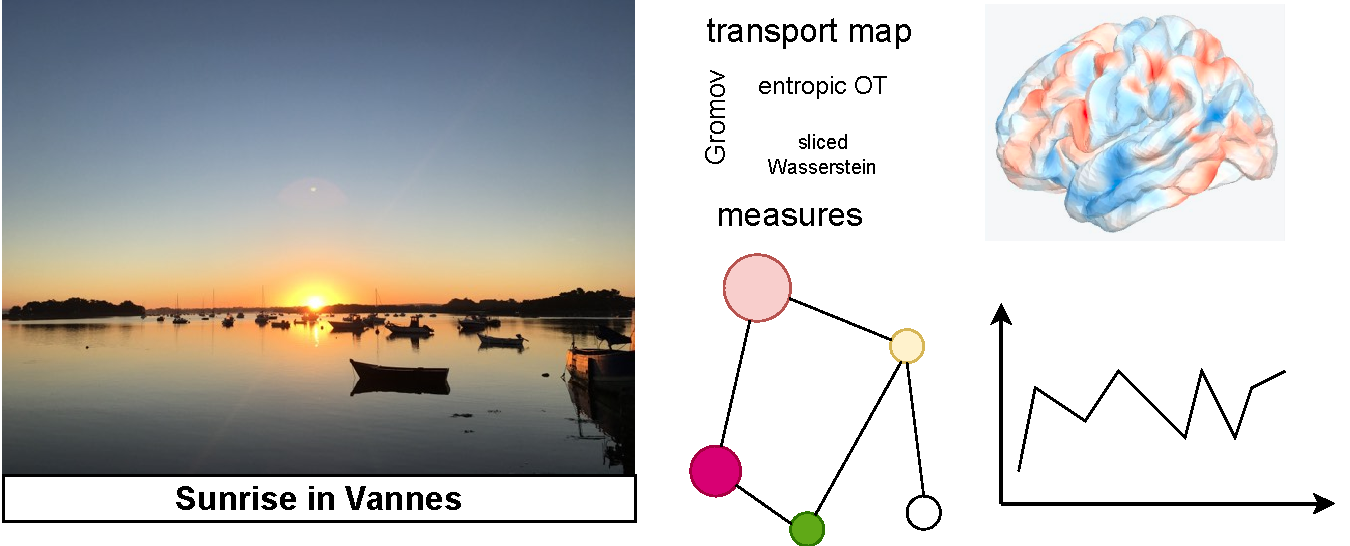
\includegraphics[width=1.15\linewidth, keepaspectratio=true]{OT_new/appli.pdf}
  \end{figure}
  \end{minipage}

\end{frame}

%%%%%%%%%%%%%%%%%%%%%%%%%%%%%%%%%%%%%%%%%%%%%%
% \begin{frame}{Why Gromov-Wasserstein distance?}
% \scriptsize
%   \begin{align*}
%     d_{H} \big( {\color{blue}{(X, d)}}, {\color{red}{(Y, d)}} \big)
%     = \inf_{R \in \mathcal R({\color{blue}{X}}, {\color{red}{Y}})}
%     \sup_{(x, y) \in R} d(x, y)
%   \end{align*}

%   \begin{align*}
%     W_{\infty}\big( {\color{blue}{(X, \mu_X, d)}}, {\color{red}{(Y, \mu_Y, d)}} \big) =
%     \inf_{\pi \in U({\color{blue}{\mu_X}}, {\color{red}{\mu_Y}})} \sup_{(x,y) \in \text{supp}(\pi)}
%     d(x, y)
%   \end{align*}

%   \begin{align*}
%     W_p^p \big( {\color{blue}{(X, \mu_X, d)}}, {\color{red}{(Y, \mu_Y, d)}} \big)
%     = \inf_{\pi \in U({\color{blue}{\mu_X}}, {\color{red}{\mu_Y}})}
%     \int d(x, y)^p \; \rmd\pi(x, y).
%   \end{align*}

%   \begin{align*}
%     \gh\big( {\color{blue}{(X, d_X)}}, {\color{red}{(Y, d_Y)}} \big)
%     = \frac{1}{2} \inf_{R \in \mathcal R({\color{blue}{X}}, {\color{red}{Y}})}
%     \sup_{\substack{(x_1,y_1) \in R \\ (x_2,y_2) \in R}} \big| d_X(x_1, x_2) - d_Y(y_1, y_2) \big|
%   \end{align*}

%   \begin{align*}
%     \gw_{\infty}\big( {\color{blue}{(X, \mu_X, d_X)}}, {\color{red}{(Y, \mu_Y, d_Y)}} \big)
%     = \inf_{ \pi \in U({\color{blue}{\mu_X}}, {\color{red}{\mu_Y}})}
%     \sup_{\substack{(x_1,y_1) \in \text{supp}(\pi) \\ (x_2,y_2) \in \text{supp}(\pi)}}
%     \big| d_X(x_1, x_2) - d_Y(y_1, y_2) \big|.
%   \end{align*}

%   \begin{align*}
%     \gw_p^p\big( {\color{blue}{(X, \mu_X, d_X)}}, {\color{red}{(Y, \mu_Y, d_Y)}} \big)
%     = \inf_{ \pi \in U({\color{blue}{\mu_X}}, {\color{red}{\mu_Y}})}
%     \iint |d_X(x_1, x_2) - d_Y(y_1, y_2)|^p \;
%     \rmd\pi(x_1, y_1) \; \rmd\pi(x_2, y_2).
% \end{align*}
% \end{frame}

%%%%%%%%%%%%%%%%%%%%%%%%%%%%%%%%%%%%%
\begin{frame}{Optimal transport across-space}
  \vspace{-0cm}
  \scriptsize
  \begin{block}{Gromov-Wasserstein distance \parencite{Memoli07,Memoli11}}
  The GW distance of order $p \geq 1$ between two metric-measure spaces
  $\cX_1 = (X_1, \mu_1, d_1)$ and $\cX_2 = (X_2, \mu_2, d_2)$ is defined as
  \begin{align*}
    \gw_p^p(\cX_1, \cX_2) = \inf_{\pi \in U(\mu_1, \mu_2)}
    \iint \left| d_1(x_1, x_1') - d_2(x_2, x_2') \right|^p
    \rmd\pi(x_1, x_2) \; \rmd\pi(x_1', x_2'),
  \end{align*}
  where $U(\mu_1, \mu_2) = \{ \pi \in \mathcal P(X_1 \times X_2): \int_{X_2} \rmd\pi(\cdot, x_2) = \mu_1 \text{ and } \int_{X_1} \rmd\pi(x_1, \cdot) = \mu_2 \}$.
\end{block}

\begin{tikzpicture}[remember picture, overlay]
  \node[shift={(-3.7cm,-6cm)}] at (current page.center)
  {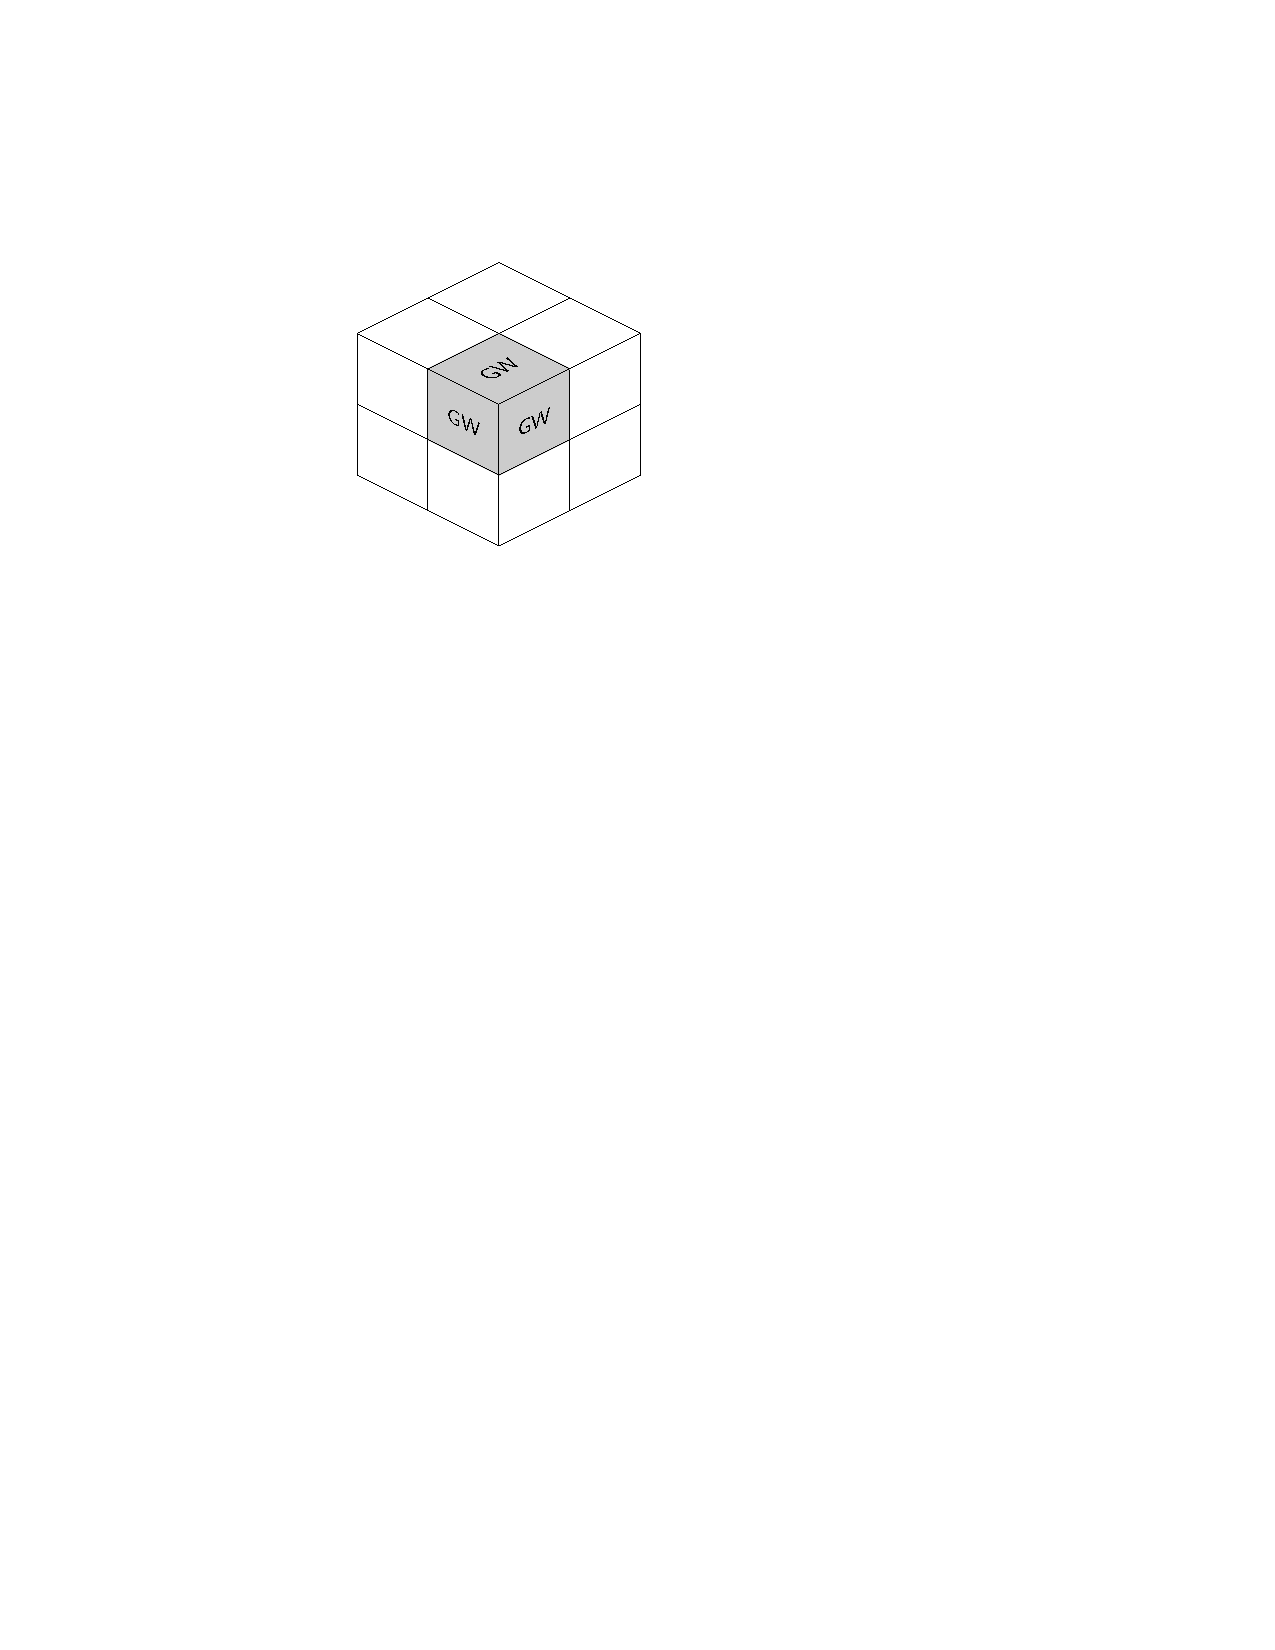
\includegraphics[scale=0.35]{OT_new/cube_gw.pdf}};
\end{tikzpicture}

\vspace{-0.3cm}
\begin{minipage}[t]{0.5\linewidth}
\begin{enumerate}
  \item Metric properties + isometries.
  \item Not the only way to compare incomparable spaces

  $\Rightarrow$ Godfather: Gromov-Hausdorff dist.
  \item Computationally feasible.
  \item Many extensions.
\end{enumerate}
\end{minipage}%
\hfill%
\hspace{-6cm}
\begin{minipage}[t]{0.5\linewidth}
  \vspace{0.5cm}
\begin{figure}
  \centering
  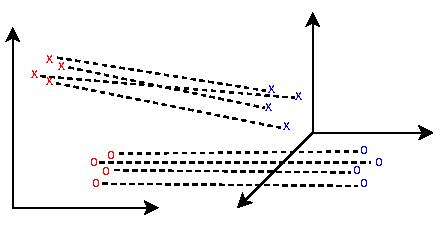
\includegraphics[width=1.15\linewidth, keepaspectratio=true]{OT_new/gw.pdf}
\end{figure}
\end{minipage}

\end{frame}

%%%%%%%%%%%%%%%%%%%%%%%%%%%%%%%%%%%%%
\begin{frame}{Extension 1: Marginal relaxation}
  \vspace{-0.5cm}
  \scriptsize
  \begin{definition}[Unbalanced GW \parencite{Sejourne20}]
    Given a Csiszár divergence $D_{\varphi}$ and $\lambda_1, \lambda_2 > 0$,
    the unbalanced GW divergence between two compact metric-measure spaces
    $\cX_1 = (X_1, \mu_1, d_1)$ and $\cX_2 = (X_2, \mu_2, d_2)$ is defined as
    \begin{align*}
      \ugw_p^p(\cX_1, \cX_2) = \inf_{\pi \in \cM^+(X_1 \times X_2)} \cL_{\ugw}(\pi),
    \end{align*}
    \vspace{-0.3cm}
    where
    \vspace{-0.5cm}
    \begin{align*}
      \cL_{\ugw}(\pi) &= \iint \left| d_1(x_1, x_2) - d_2(y_1, y_2) \right|^p
      \rmd\pi(x_1, y_1) \; \rmd\pi(x_2, y_2) \\
      &+ \lambda_1 D_{\varphi}(\pi_{\# 1} \otimes \pi_{\# 1} | \mu_1 \otimes \mu_1)
      + \lambda_2 D_{\varphi}(\pi_{\# 2} \otimes \pi_{\# 2} | \mu_2 \otimes \mu_2).
    \end{align*}
  \end{definition}

  \vspace{-0.5cm}
  \begin{tikzpicture}[remember picture, overlay]
    \node[shift={(-3.7cm,-6cm)}] at (current page.center)
    {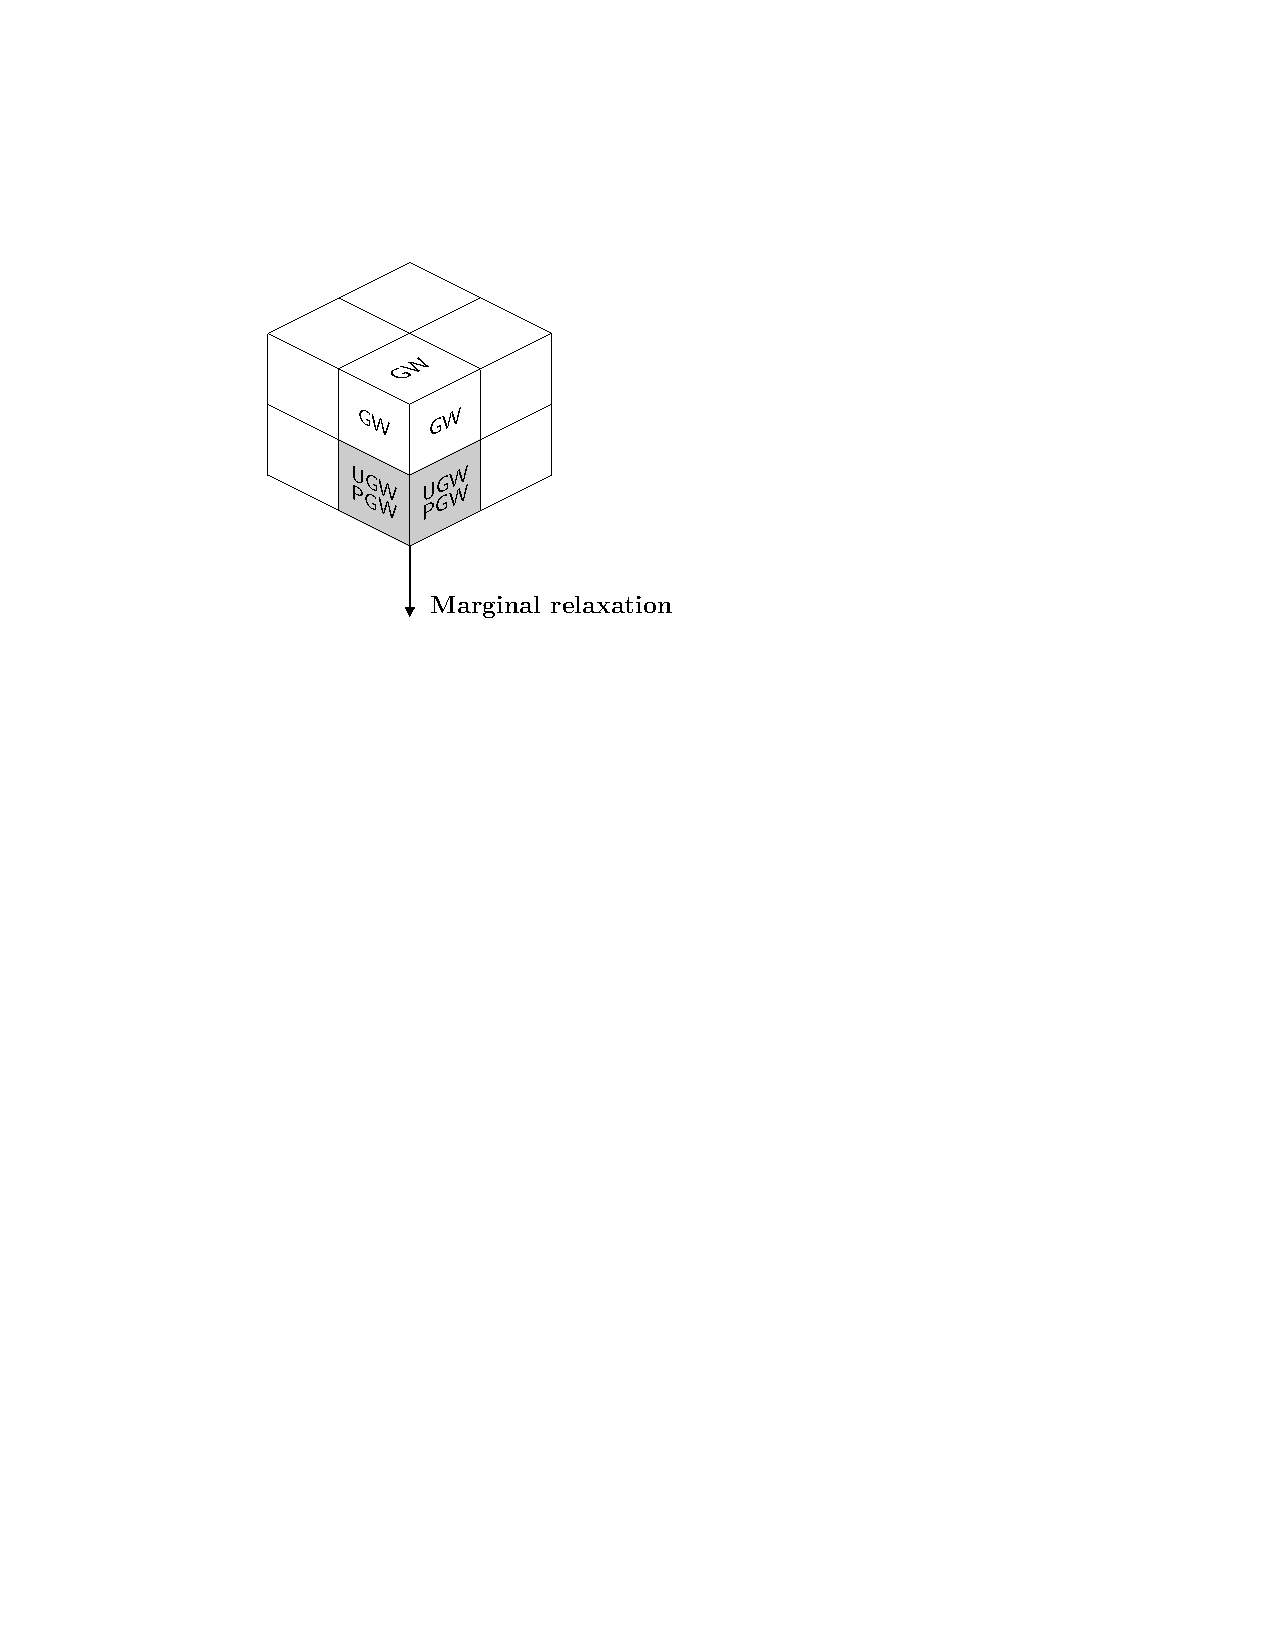
\includegraphics[scale=0.35]{OT_new/cube_ugw.pdf}};
  \end{tikzpicture}

  \begin{minipage}[t]{0.6\linewidth}
  \begin{itemize}
    \item In practice: $D_{\varphi} = \text{Kullback-Leibler div}$.
    \item Quadratic divergence $\Rightarrow$ Homogeneity:
    $\ugw_p^p(t\cX_1, t \cX_2) = t^2 \; \ugw_p^p(\cX_1, \cX_2)$,

    for $t \cX := (X, t\mu, d)$.
    \item Characterizing isometries.
  \end{itemize}
  \end{minipage}%
  \hfill%
  \hspace{-6cm}
  \begin{minipage}[t]{0.5\linewidth}
    \vspace{-0.cm}
  \begin{figure}
    \centering
    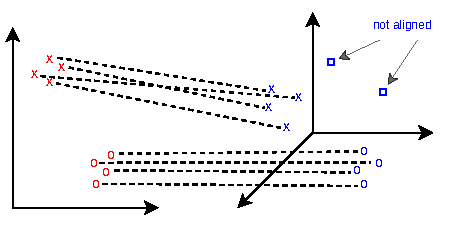
\includegraphics[width=1.1\linewidth, keepaspectratio=true]{OT_new/ugw.pdf}
  \end{figure}
  \end{minipage}

\end{frame}

%%%%%%%%%%%%%%%%%%%%%%%%%%%%%%%%%%%%%
\begin{frame}{Extension 2: Shared space}
  \scriptsize
  \begin{definition}[Fused GW \parencite{Vayer19b}]
    For $\alpha \in [0, 1]$, the fused GW between two attributed graphs
    $\cX_1 = (D_1, F_1, \mu_1)$ and $\cX_2 = (D_2, F_2, \mu_2)$,
    where $D_k \in \bbR^{n_k \times n_k}, F_k \in \bbR^{n_k \times d}$
    and $\mu_k \in \Delta_{n_k}$, is defined as
    \begin{align*}
      \fgw_p^p(\cX_1, \cX_2) = \inf_{\pi \in U(\mu_1, \mu_2)} \cL_{\fgw}(\pi),
    \end{align*}
    \vspace{-0.3cm}
    where
    \begin{align*}
      \cL_{\fgw}(\pi) = (1 - \alpha)
      \sum_{{\color{blue}{i}},{\color{blue}{j}},{\color{red}{k}},{\color{red}{l}}}
      |(D_1)_{{\color{blue}{i}} {\color{red}{k}}} - (D_2)_{{\color{blue}{j}}{\color{red}{l}}}|^p {\color{blue}{\pi_{ij}}} {\color{red}{\pi_{kl}}}
      + \alpha \sum_{ij} ||(F_1)_i - (F_2)_j||^q \pi_{ij}.
    \end{align*}
  \end{definition}

  \begin{tikzpicture}[remember picture, overlay]
    \node[shift={(-3.7cm,-6cm)}] at (current page.center)
    {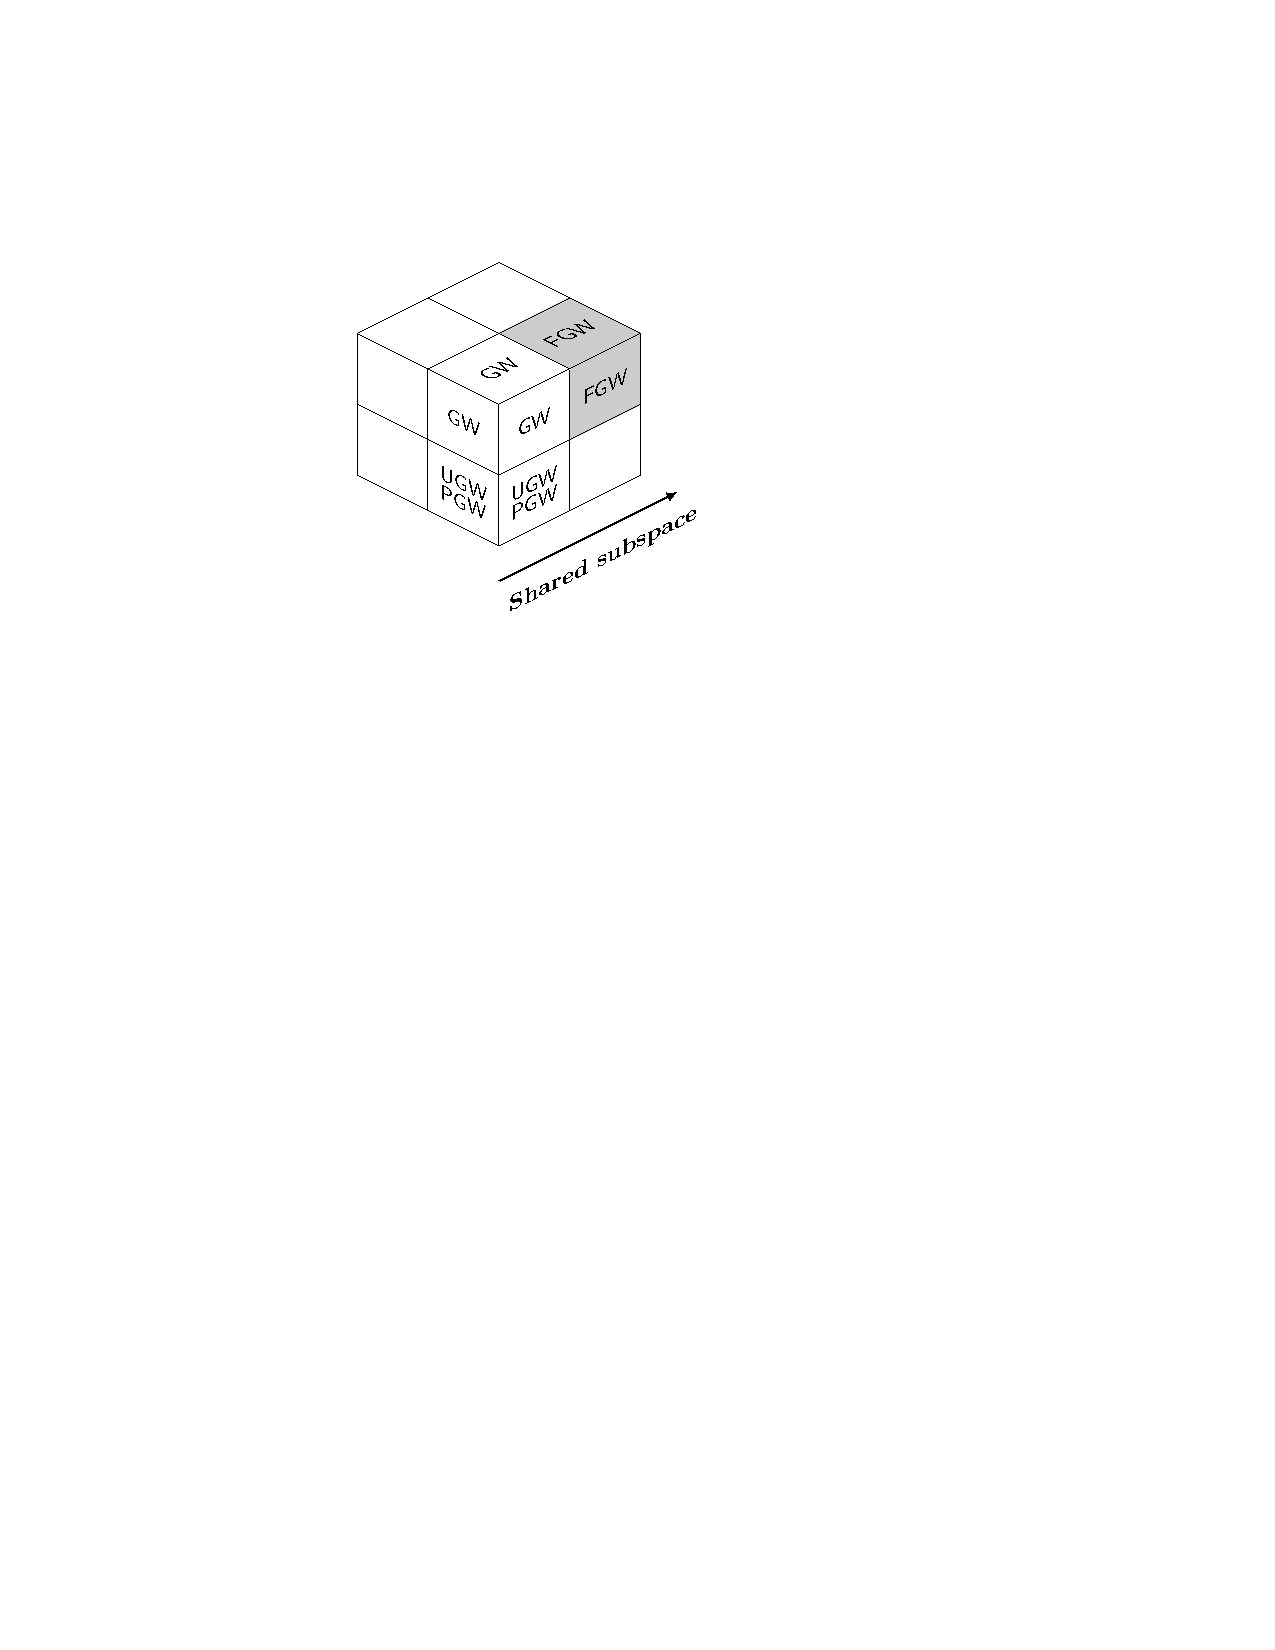
\includegraphics[scale=0.35]{OT_new/cube_fgw.pdf}};
  \end{tikzpicture}

  \begin{minipage}[t]{0.6\linewidth}
    \begin{itemize}
      \item Interpolation between GW and Wasserstein distances.
      \item Feature-preserving isometries.
    \end{itemize}
    \end{minipage}%
    \hfill%
    \hspace{-6cm}
    \begin{minipage}[t]{0.45\linewidth}
      \vspace{-0.cm}
    \begin{figure}
      \centering
      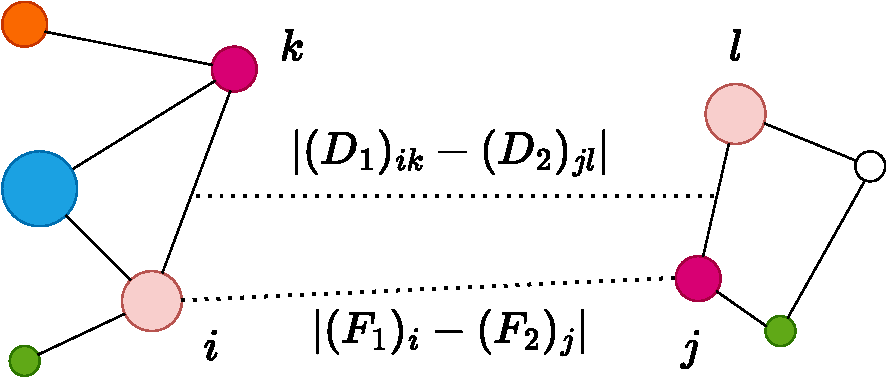
\includegraphics[width=\linewidth, keepaspectratio=true]{OT_new/fgw.pdf}
      % \caption*{\scriptsize{Inspired by \parencite{Vayer19b}}}
    \end{figure}
    \end{minipage}

\end{frame}

%%%%%%%%%%%%%%%%%%%%%%%%%%%%%%%%%%%%%
\begin{frame}{Extension 3: Bilinear relaxation}
\scriptsize

\begin{definition}[Discrete COOT \parencite{Redko20}]
  The Co-Optimal Transport distance between
  two weighted matrices $\cX_1 = (X_1, \mssrc, \mfsrc)$
and $\cX_2 = (X_2, \mstg, \mftg)$, where
$X_k \in \bbR^{n_k \times d_k}$ and histograms
${\color{blue}{\mu^s_k \in \Delta_{n_k}}}, {\color{red}{\mu^f_k \in \Delta_{d_k}}}$,
is defined as
\begin{align*}
  \coot_p^p(\cX_1, \cX_2) =
  \min_{\substack{\pis \in U(\mssrc,\mstg) \\ \pif \in U(\mfsrc,\mftg)}}
  \sum_{{\color{blue}{i}},{\color{blue}{j}},{\color{red}{k}},{\color{red}{l}}}
  |(X_1)_{{\color{blue}{i}} {\color{red}{k}}} - (X_2)_{{\color{blue}{j}}{\color{red}{l}}}|^p {\color{blue}{\pi^s_{ij}}} {\color{red}{\pi^f_{kl}}}
\end{align*}
\end{definition}

\begin{tikzpicture}[remember picture, overlay]
  \node[shift={(-3.7cm,-6cm)}] at (current page.center)
  {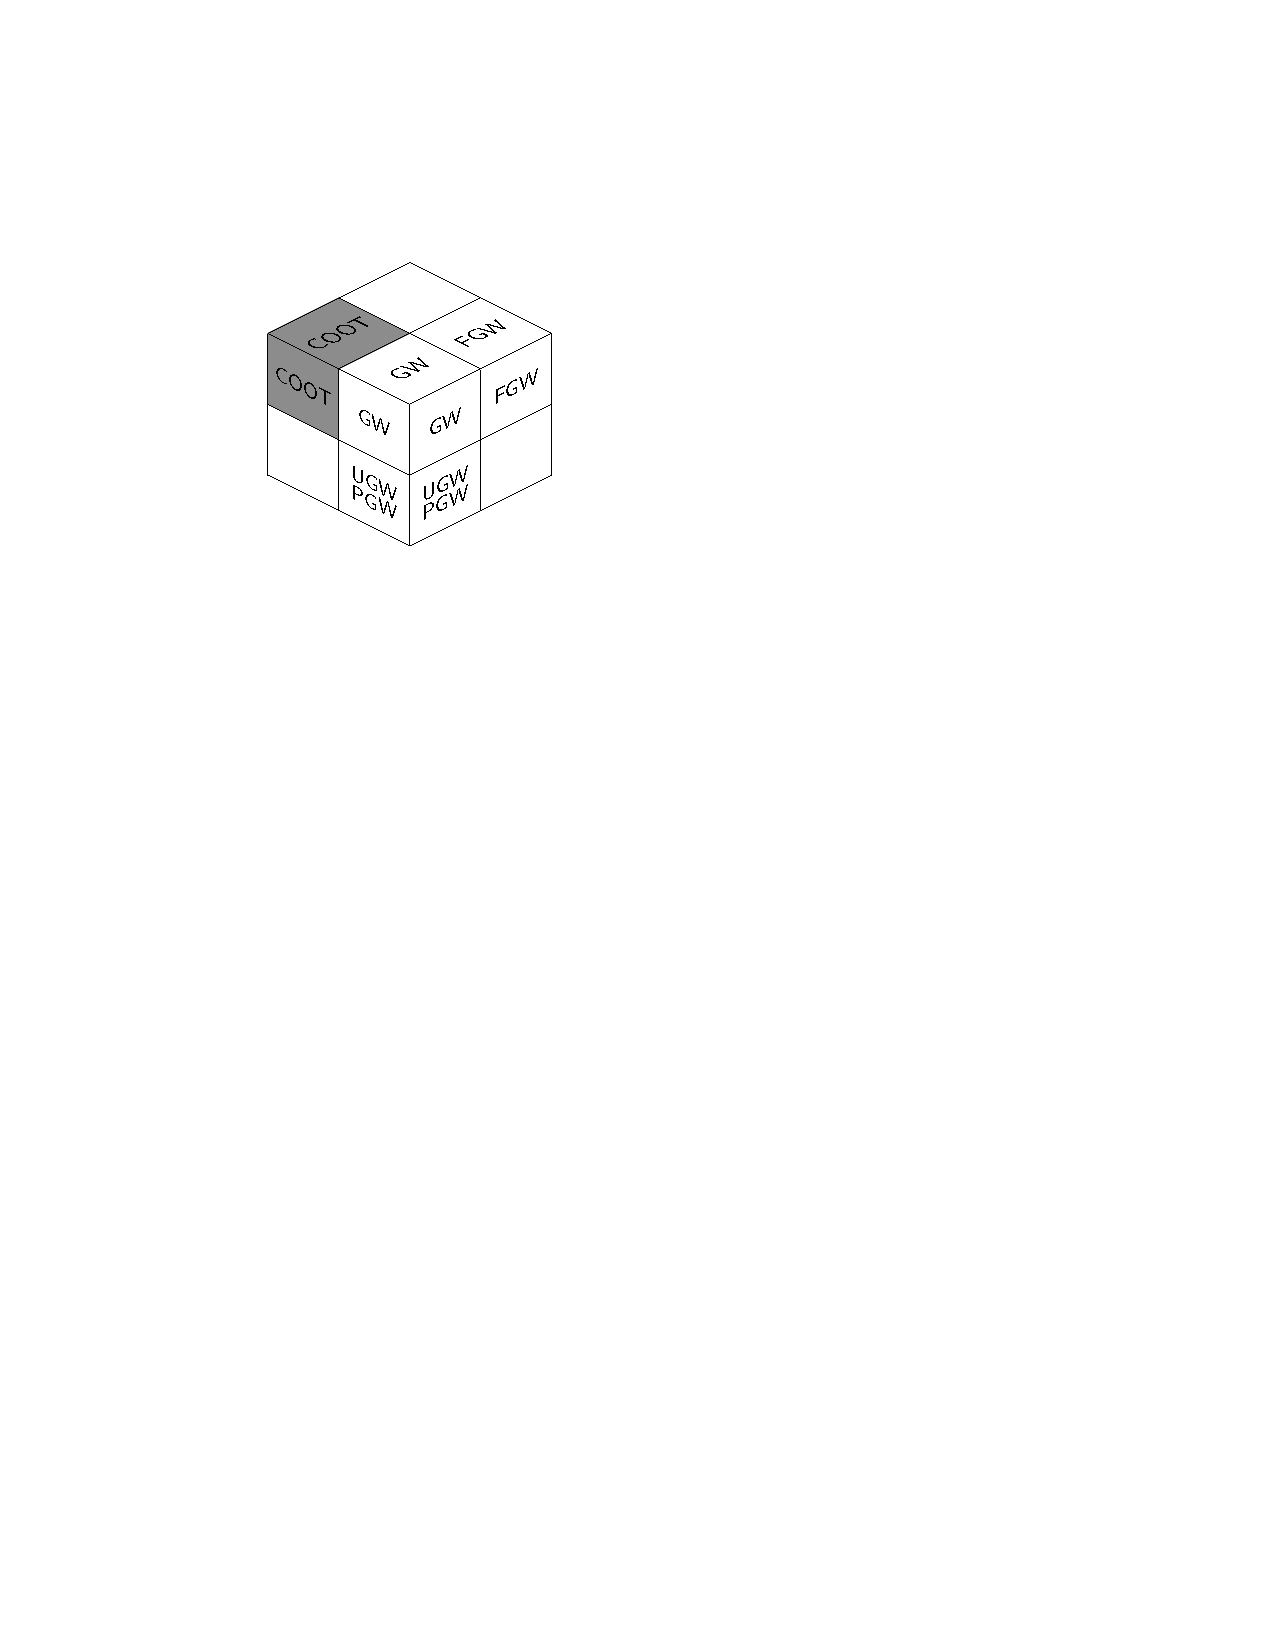
\includegraphics[scale=0.35]{OT_new/cube_coot.pdf}};
\end{tikzpicture}

\vspace{-0.3cm}
\begin{minipage}[t]{0.6\linewidth}
  \begin{itemize}
    \item Comparing \underline{arbitrary-size} matrices.
    \item Continuous extension \parencite{Chowdhury21b}.
    \item Meaningful {\color{red}{feature}} coupling $\pif$.
    \item Metric properties.
    \item Connection with GW distance.
  \end{itemize}
  \end{minipage}%
  \hfill%
  \hspace{-6cm}
  \begin{minipage}[t]{0.55\linewidth}
    \vspace{0.5cm}
  \begin{figure}
    \centering
    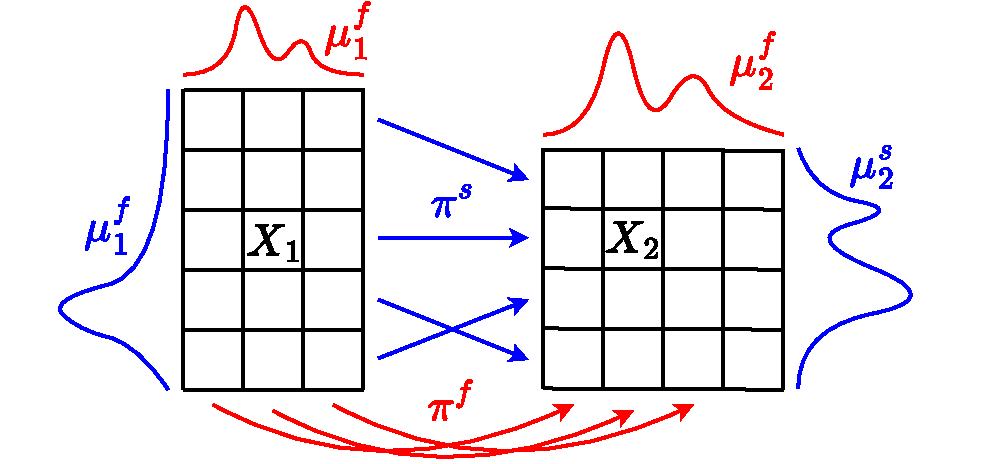
\includegraphics[width=1.15\linewidth, keepaspectratio=true]{OT_new/coot_matrix_ot.pdf}
  \end{figure}
  \end{minipage}
\end{frame}

%%%%%%%%%%%%%%%%%%%%%%%%%%%%%%%%%%%%%%%%%%%
\begin{frame}{Summary of contributions}
  \scriptsize
  \begin{tikzpicture}[remember picture, overlay]
    \node[shift={(4cm,-7.5cm)}] at (current page.center)
    {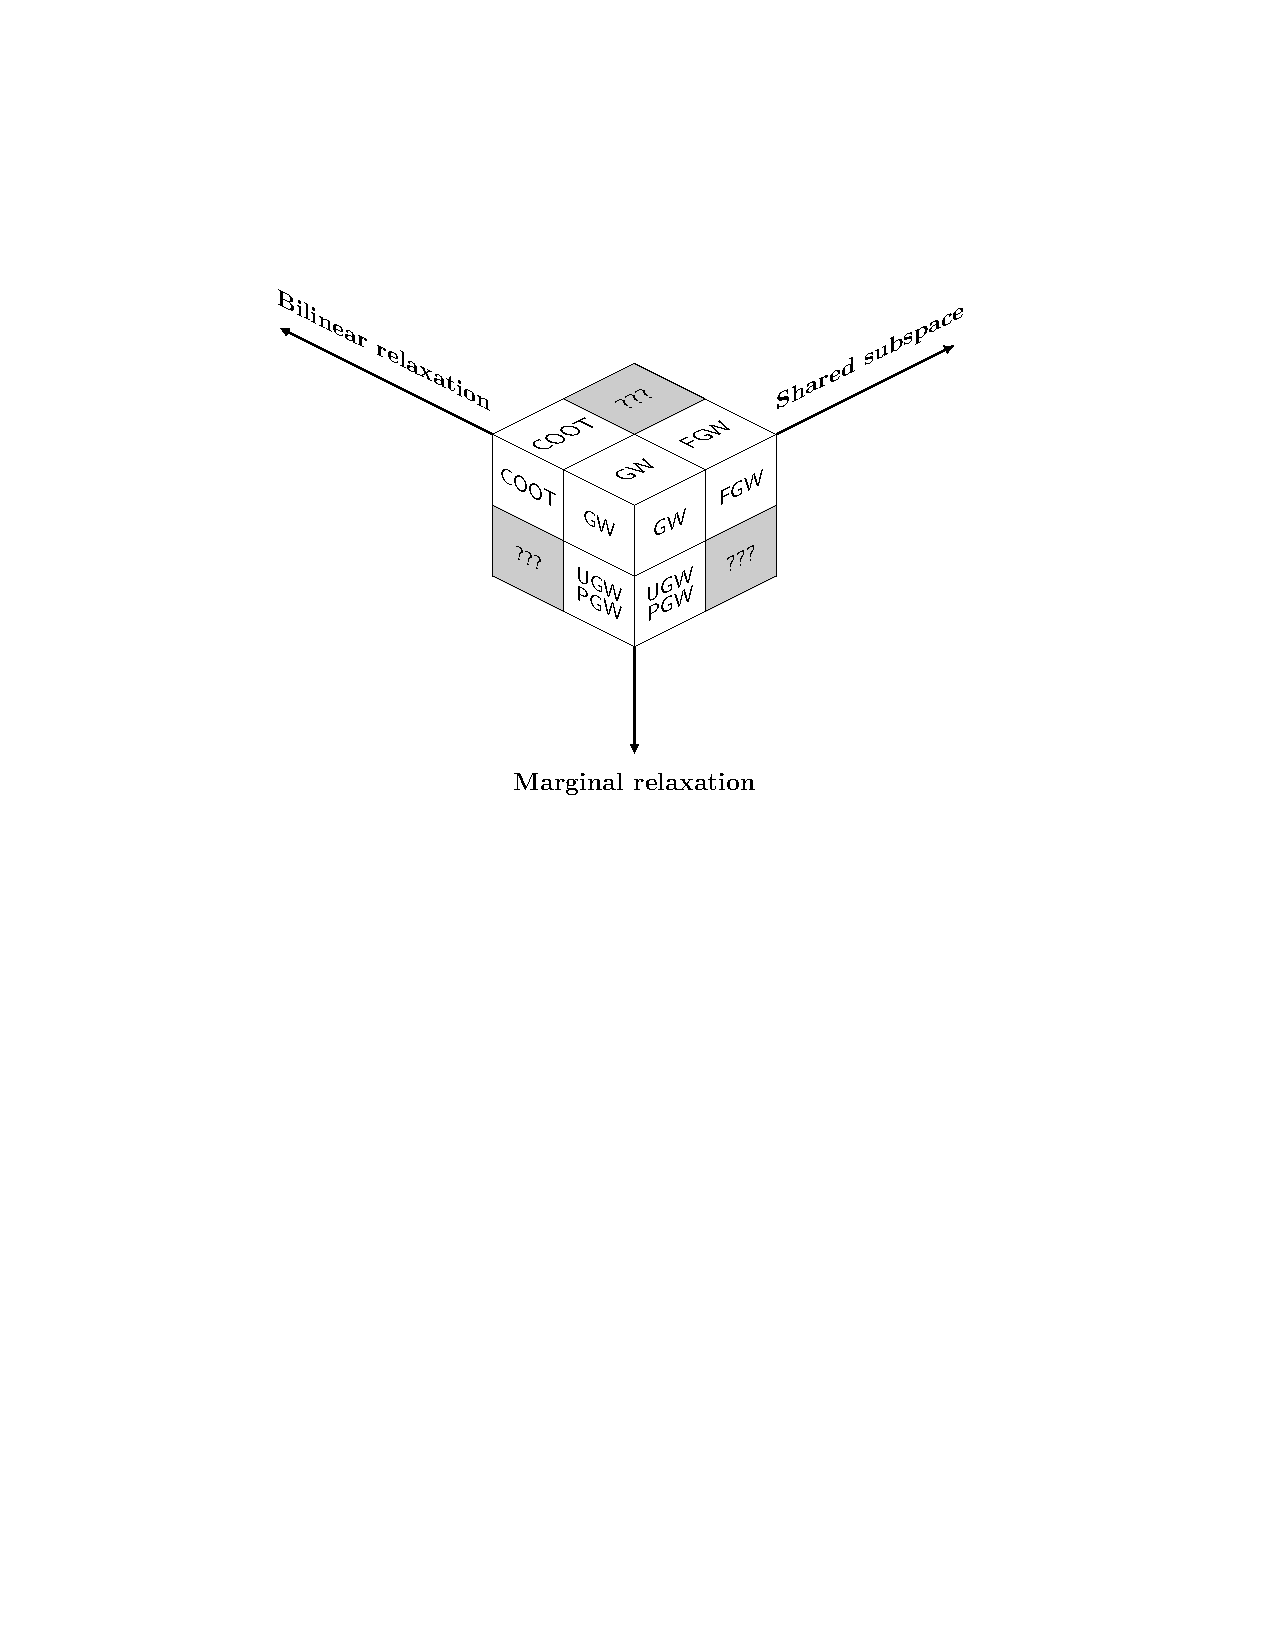
\includegraphics[scale=1]{OT_new/cube_intro.pdf}};
  \end{tikzpicture}

\end{frame}

%%%%%%%%%%%%%%%%%%%%%%%%%%%%%%%%%%%%%%%%
%%%%%%%%%%%%%%%%%%%%%%%%%%%%%%%%%%%%%%%%
%%%% Contribution on FUGW
\section{Fused Unbalanced Gromov-Wasserstein}

%%%%%%%%%%%%%%%%%%%%%%%%%%%%%%%%%%%%%%%%%%%%
\begin{frame}{Motivation}
\scriptsize
\begin{itemize}
  \item High variability in human anatomies and functional MRI responses across subjects.
  \item Lack of principled framework for brain alignments.
  \item Averaging surface brains results in loss of individual details.
\end{itemize}
\begin{figure}
  \centering
  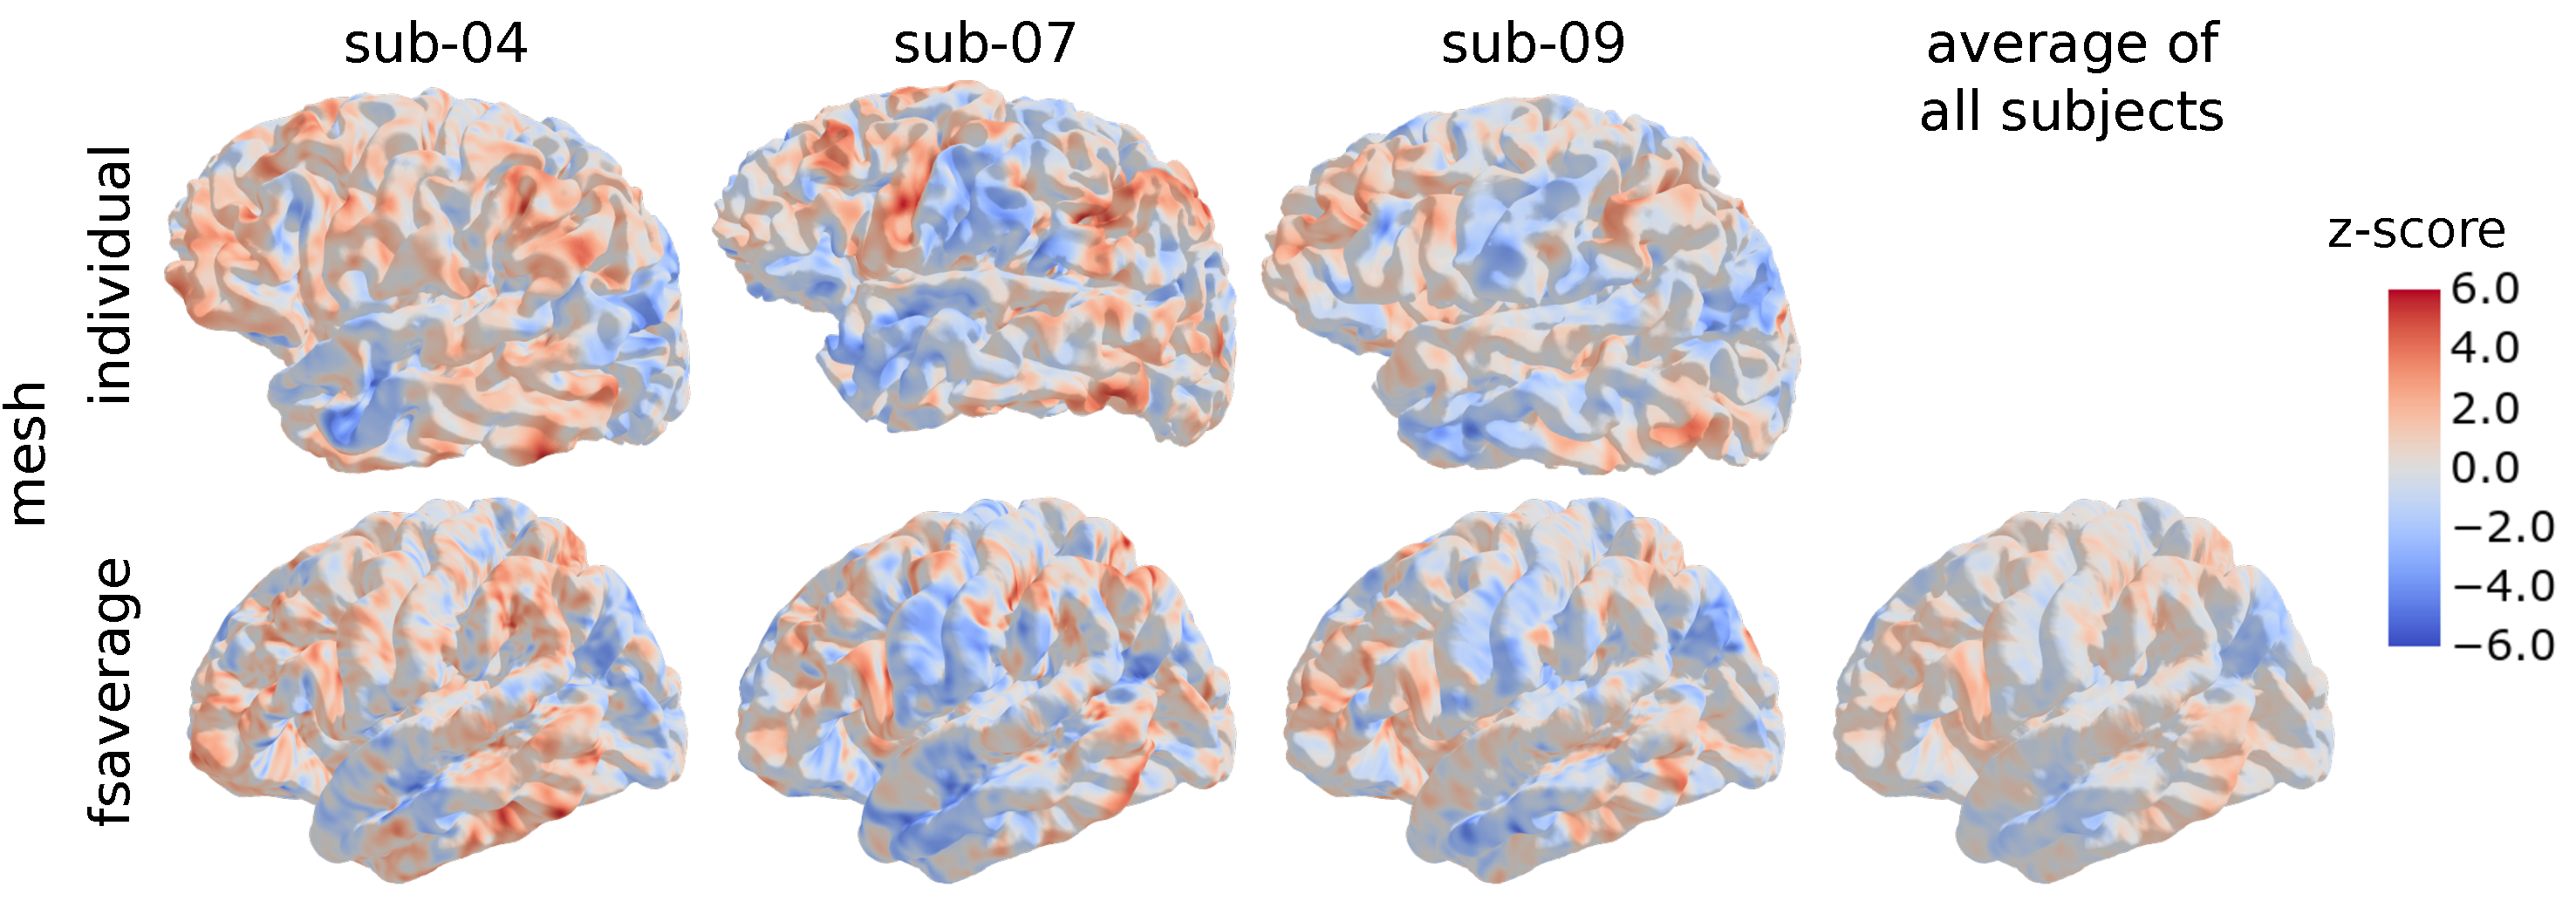
\includegraphics[width=1.\linewidth, keepaspectratio=true]{OT_new/intro_variation.pdf}
  % \caption*{\scriptsize{High variability in human anatomies and functional MRI responses across subjects.}}
\end{figure}

\begin{tikzpicture}[remember picture, overlay]
  \node[shift={(-3.7cm,-6cm)}] at (current page.center)
  {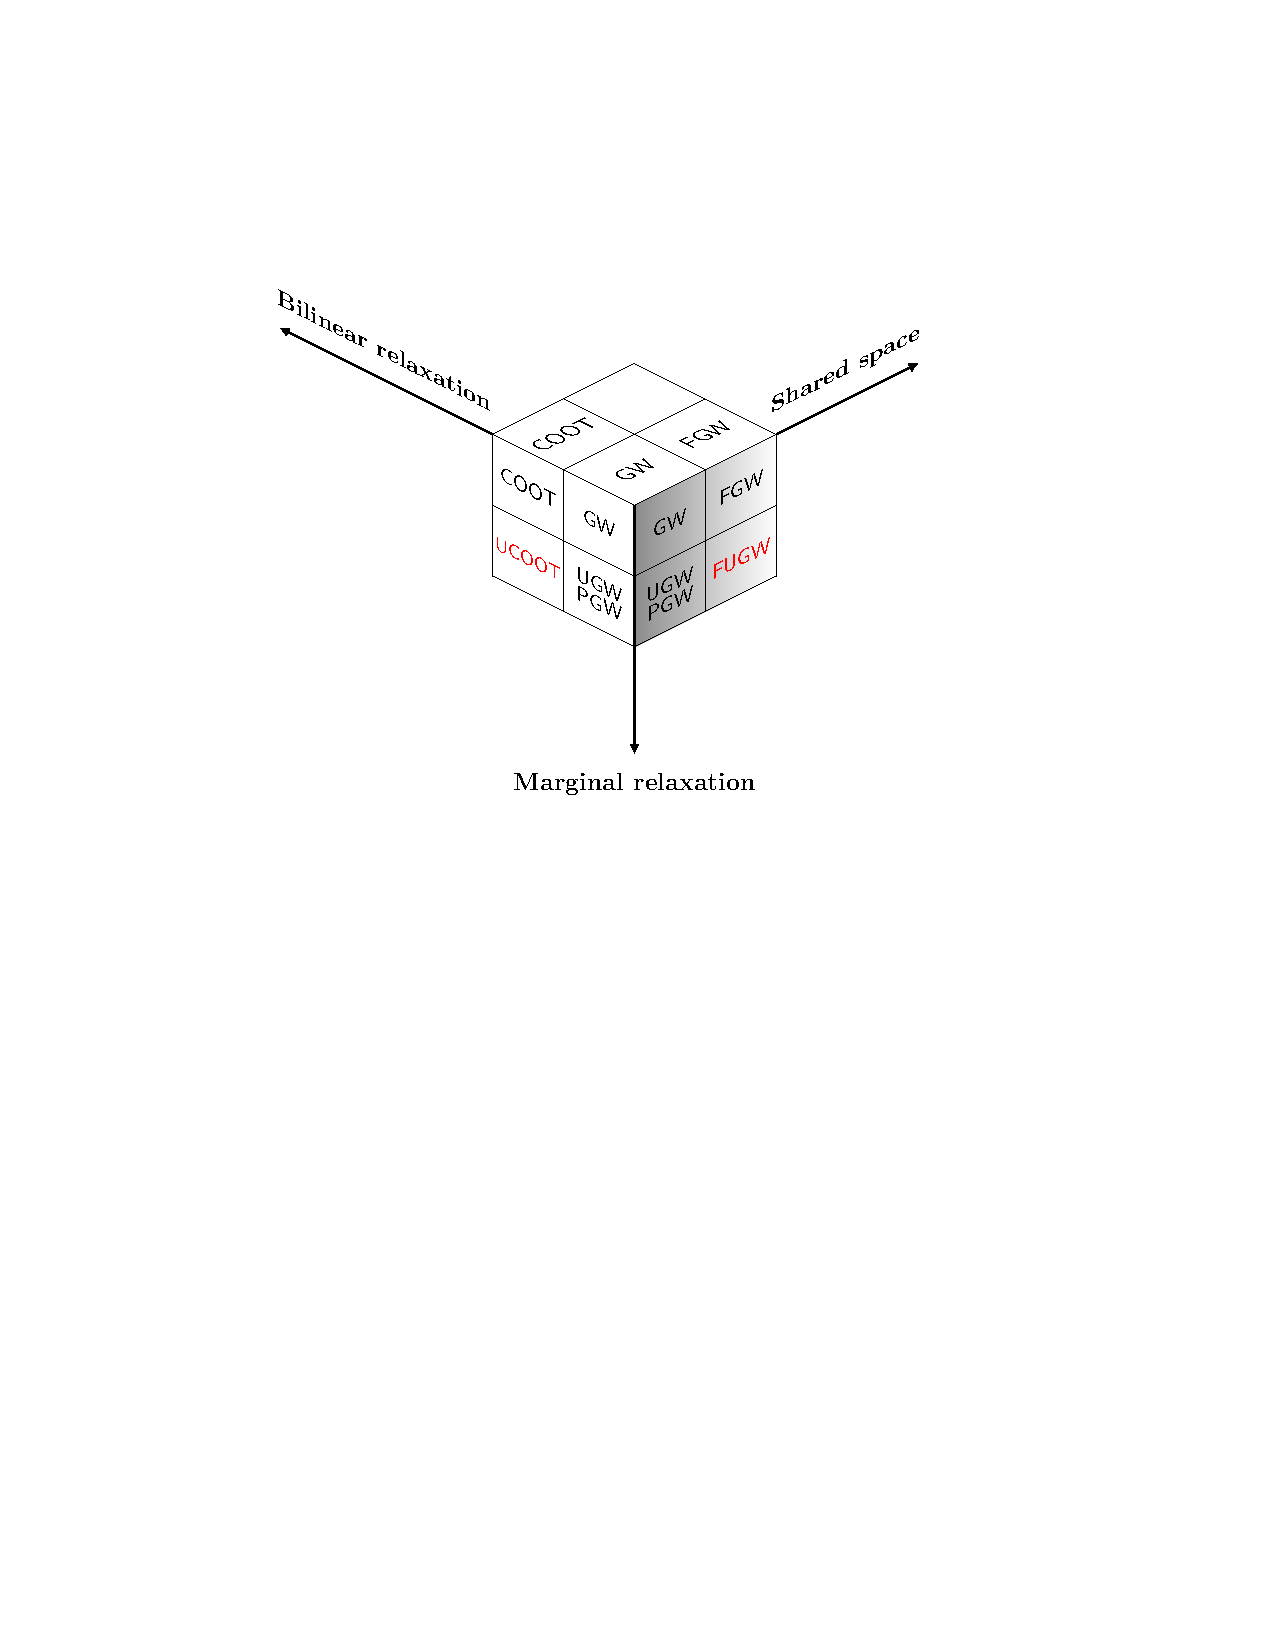
\includegraphics[scale=0.35]{OT_new/cube_fugw.pdf}};
\end{tikzpicture}

\end{frame}

%%%%%%%%%%%%%%%%%%%%%%%%%%%%%%%%%%%%%%%%%%%
\begin{frame}{Summary of contributions}
  \scriptsize

  \begin{tikzpicture}[remember picture, overlay]
    \node[shift={(0cm,-1.5cm)}] at (current page.center)
    {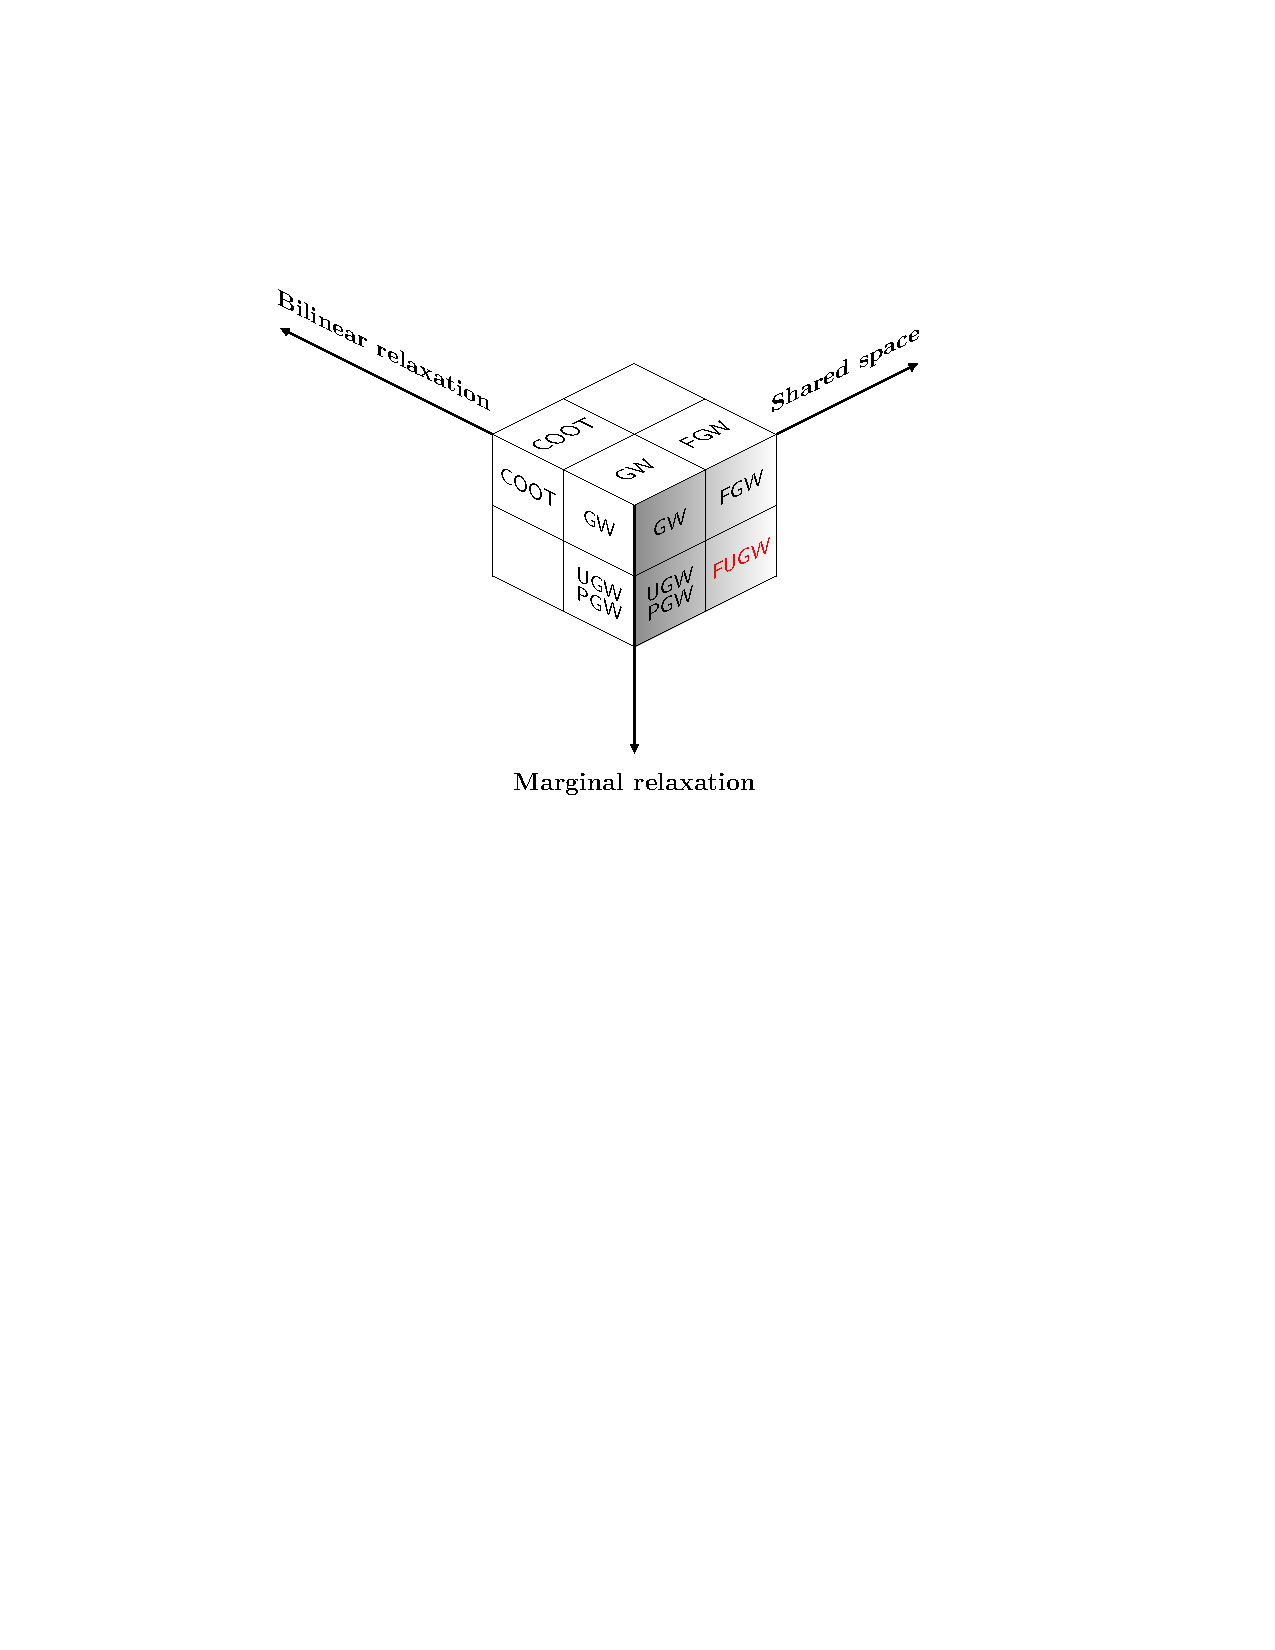
\includegraphics[scale=0.55]{OT_new/cube_fugw_contrib.pdf}};
  \end{tikzpicture}

  \vspace{5cm}
  {\color{brown}{\textbf{Summary}}}: applied fused unbalanced GW to
  \begin{enumerate}
    \item Align human cortical surfaces.
    \item Learn human brain templates.
  \end{enumerate}

  \vspace{0.3cm}
  {\color{brown}{\textbf{Publication}}}: \ul{Aligning individual brains with Fused Unbalanced Gromov-Wasserstein}.
  Alexis Thual*, \textbf{QHT}*, Tatiana Zemskova, Nicolas Courty,
  Rémi Flamary, Stanislas Dehaene, and Bertrand Thirion.
  \textit{Advances in neural information processing systems (NeurIPS)}, 2022.

\end{frame}

%%%%%%%%%%%%%%%%%%%%%%%%%%%%%%%%%%%%%%%%%%%%
\begin{frame}{Formulation}
\scriptsize
\vspace{-0.7cm}
\begin{block}{Definition}
  Given $\lambda > 0$ and $\alpha \in [0, 1]$, the fused unbalanced GW
  between two attributed graphs $\cX^s = (D^s, F^s, \mu^s)$ and
  $\cX^t = (D^t, F^t, \mu^t)$ is defined as
\begin{align*}
  \fugw(\cX^s, \cX^t) = \inf_{P \in \bbR^{m \times n}_{\geq 0}} \quad
  &(1 - \alpha) \sum_{i,j,k,l} | D^s_{ik} - D^t_{jl}|^2 P_{ij} P_{kl}
  + \alpha \sum_{i,j} || F^s_i - F^t_j||_2^2 P_{ij} \\
  &+ \lambda \Big[ \kl(P_{\# 1} \otimes P_{\# 1} \vert w^s \otimes w^s)
  + \kl(P_{\# 2} \otimes P_{\# 2} \vert w^t \otimes w^t) \Big].
\end{align*}
\end{block}

\begin{tikzpicture}[remember picture, overlay]
  \node[shift={(-3.7cm,-6cm)}] at (current page.center)
  {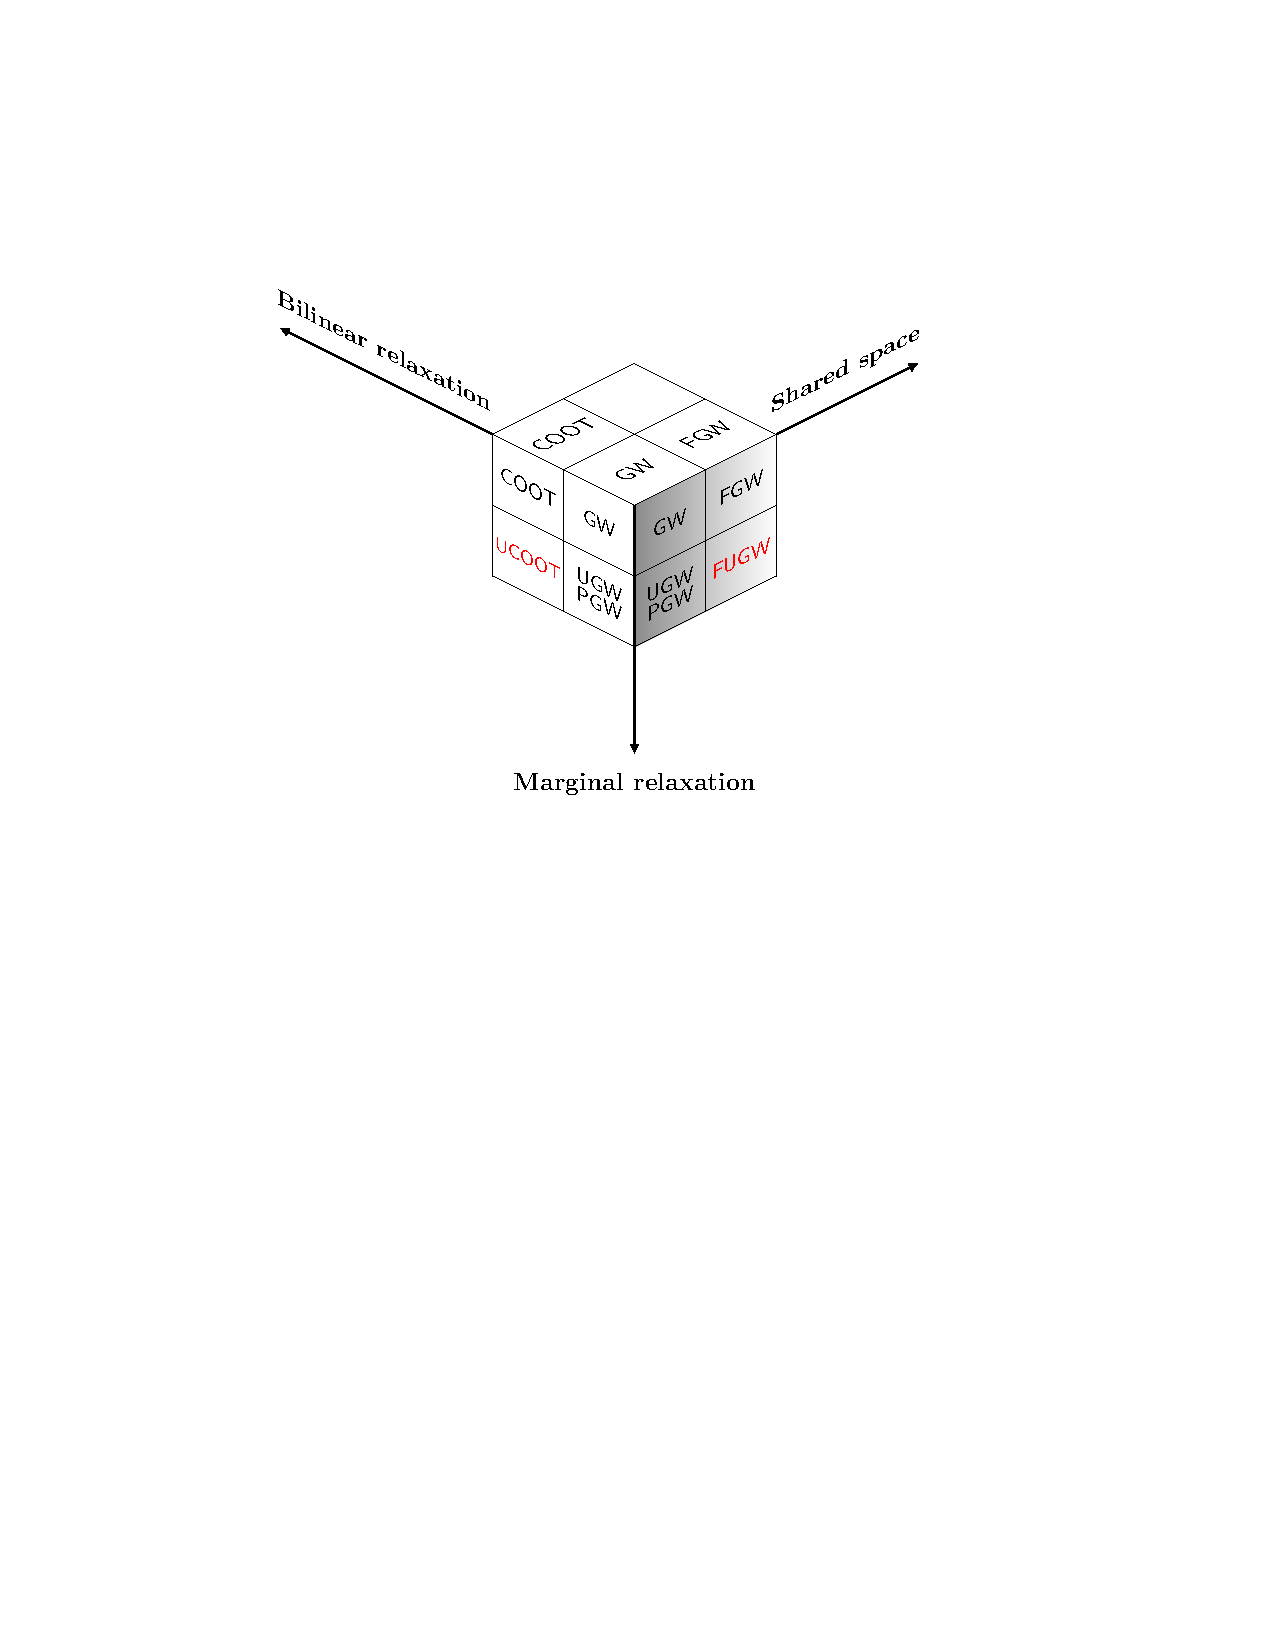
\includegraphics[scale=0.35]{OT_new/cube_fugw.pdf}};
\end{tikzpicture}

\vspace{-0.6cm}
\begin{figure}
  \centering
  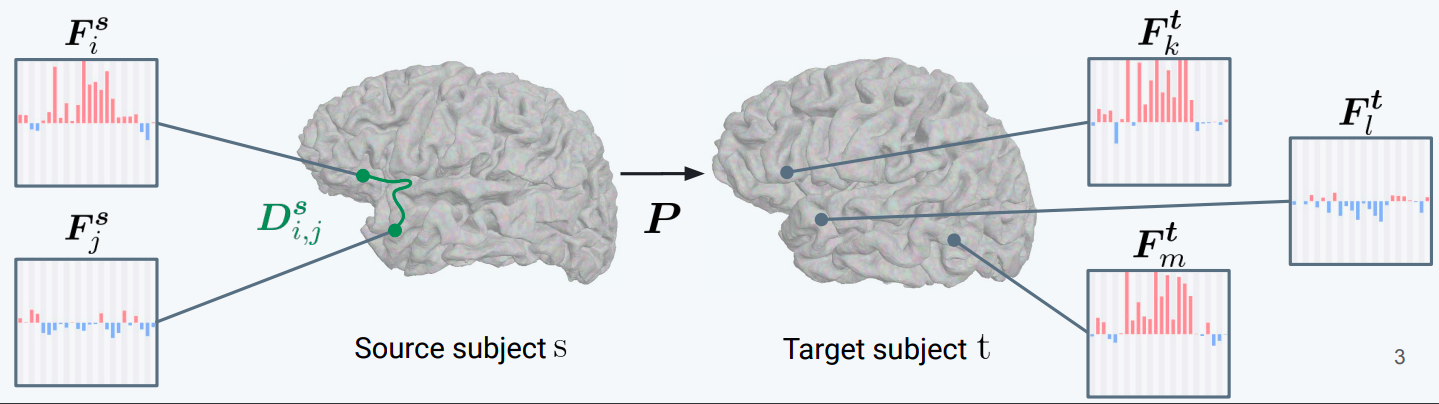
\includegraphics[width=1.\linewidth, keepaspectratio=true]{OT_new/fugw.png}
  \caption*{\scriptsize{Neuroscientific illustration of FUGW.}}
\end{figure}
\end{frame}

%%%%%%%%%%%%%%%%%%%%%%%%%%%%%
\begin{frame}{Why is unbalancing important?}
\scriptsize
\vspace{-0.5cm}
\begin{itemize}
  \item Feature = scalar.
  \item On the source mesh, the signal is constituted of two von Mises density functions that differ
  by their concentration (large and small).
  \item On the target mesh, only the large one is present, but at a different location.
\end{itemize}
\begin{figure}
  \centering
  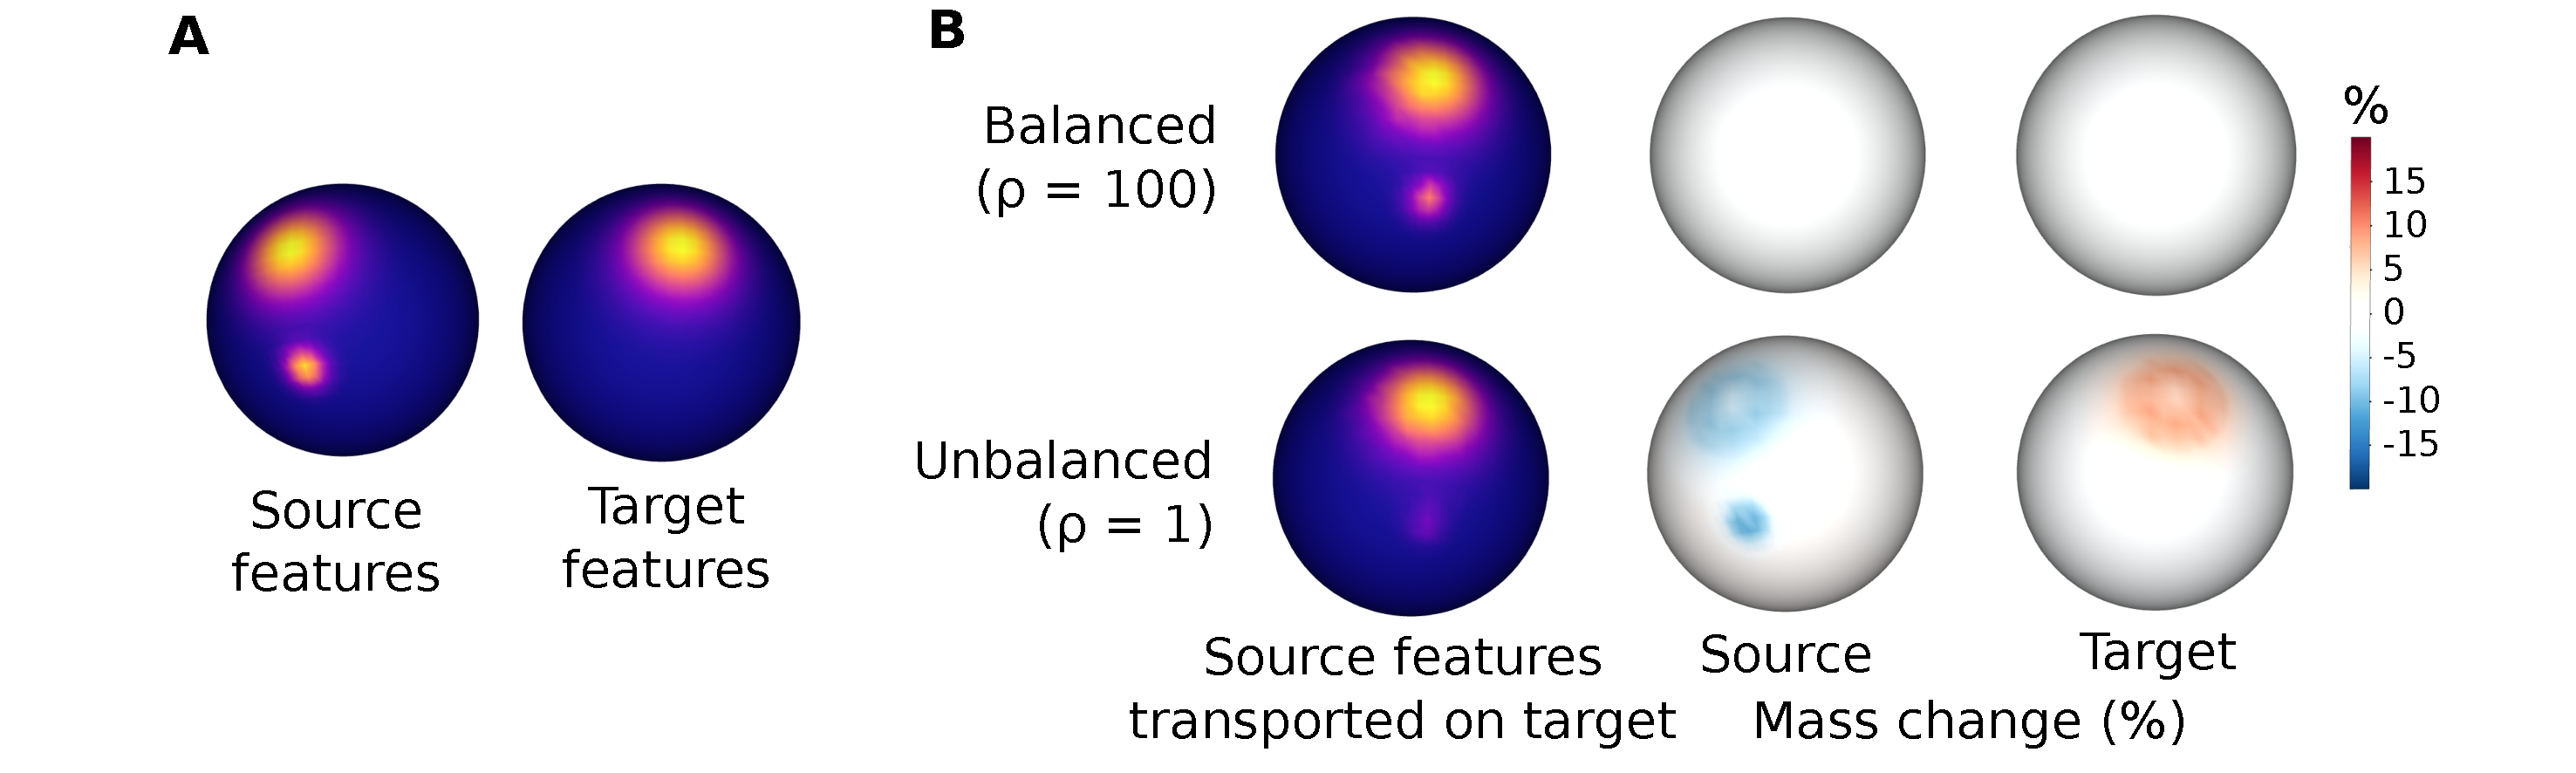
\includegraphics[width=1.\linewidth, keepaspectratio=true]{OT_new/toy_example.pdf}
  \caption*{\scriptsize{Unbalancing helps accounting for idiosyncrasies of the source and target signals.}}
\end{figure}

\begin{tikzpicture}[remember picture, overlay]
  \node[shift={(-3.7cm,-6cm)}] at (current page.center)
  {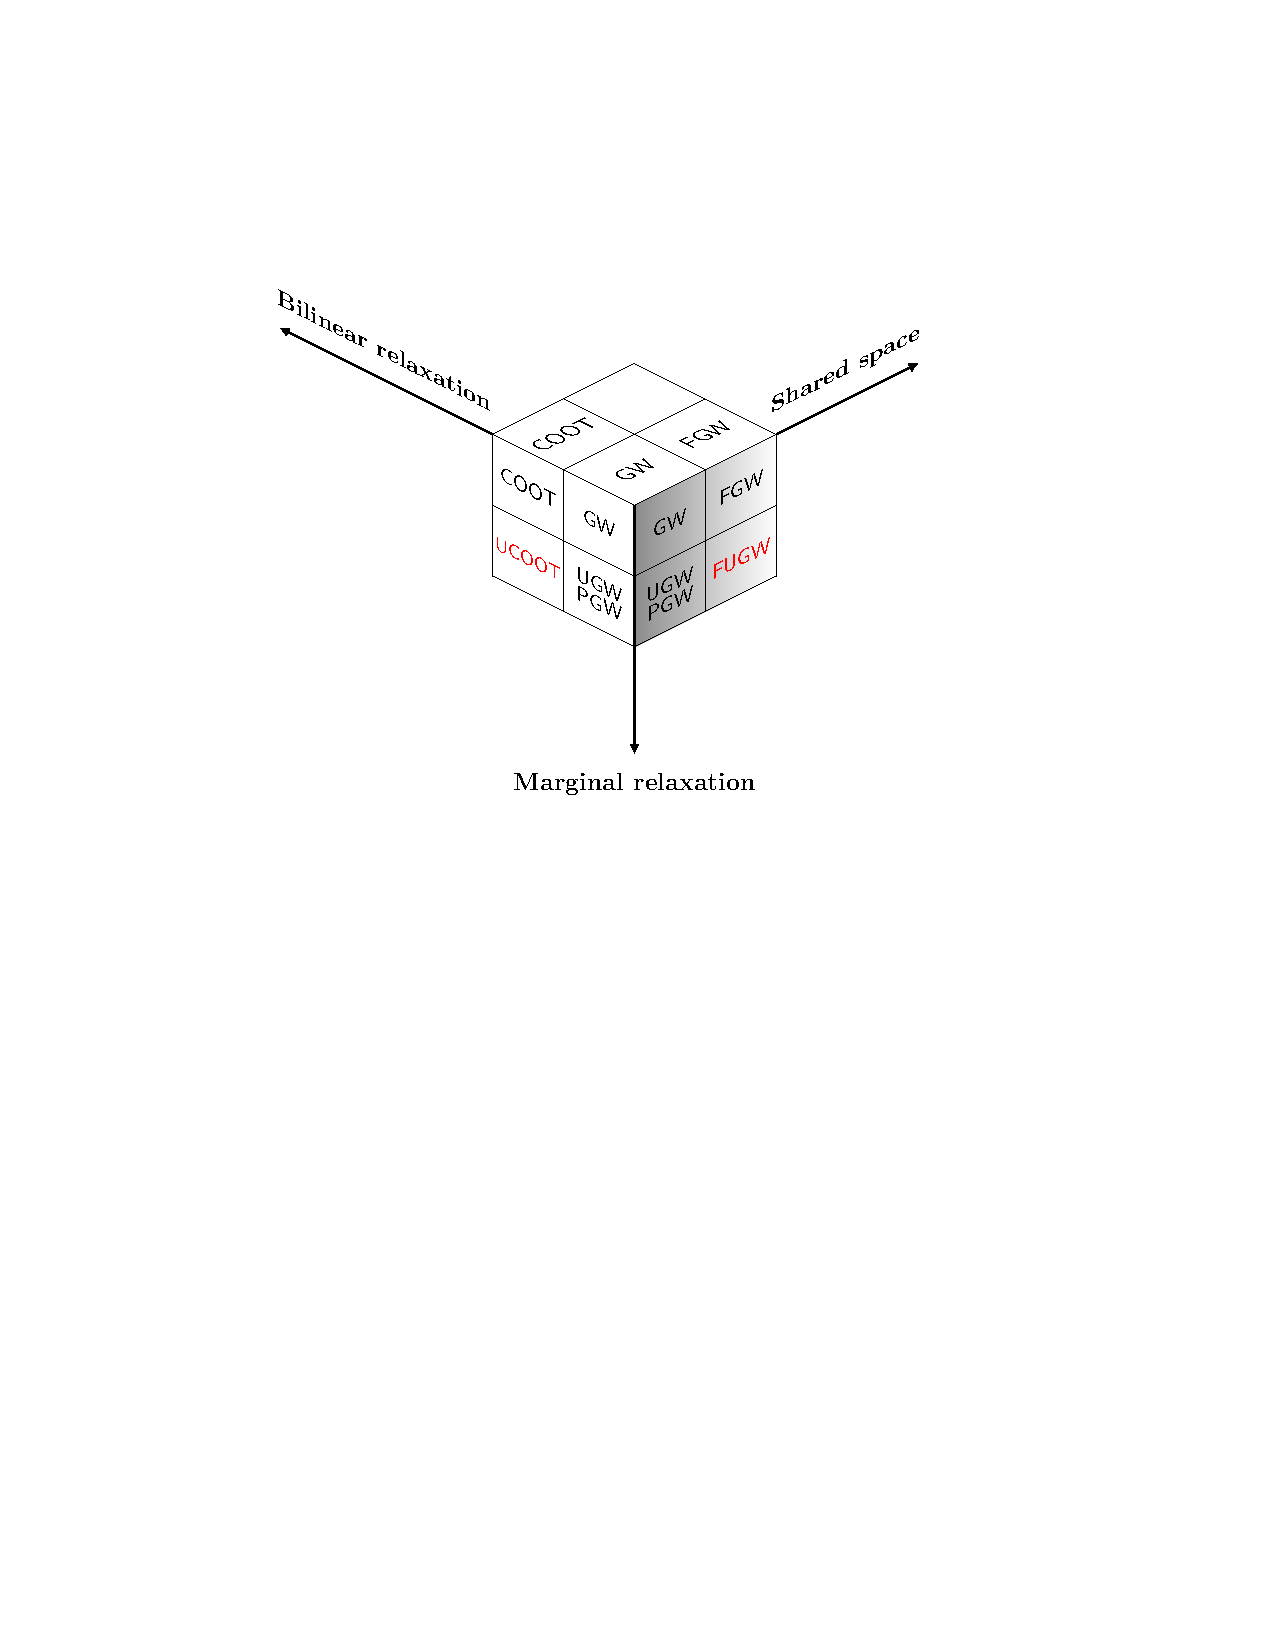
\includegraphics[scale=0.35]{OT_new/cube_fugw.pdf}};
\end{tikzpicture}

\end{frame}

%%%%%%%%%%%%%%%%%%%%%%%%%%%%%
\begin{frame}{Optimization}
\scriptsize
Denote
\vspace{-0.3cm}
\begin{align*}
  \cL_{\fugw}(P, Q) &=
  (1 - \alpha) \sum_{i,j,k,l} | D^s_{ik} - D^t_{jl}|^2 P_{ij} Q_{kl}
  + \frac{\alpha}{2} \Big[ \sum_{i,j} || F^s_i - F^t_j||_2^2 (P_{ij} + Q_{ij}) \Big] \\
  &+ \lambda \Big[ \kl(P_{\# 1} \otimes Q_{\# 1} \vert w^s \otimes w^s)
  + \kl(P_{\# 2} \otimes Q_{\# 2} \vert w^t \otimes w^t) \Big].
\end{align*}
\vspace{-0.3cm}
Then,
\begin{align*}
  \quad \fugw(\cX^s, \cX^t) = \inf_{\substack{P = Q}}
  \cL_{\fugw}(P, Q) &\geq \inf_{\substack{P_{\#1} = Q_{\#1} \\ P_{\#2} = Q_{\#2}}}
  \cL_{\fugw}(P, Q) \triangleq \widetilde{\fugw}(\cX^s, \cX^t) \\
  &\geq \inf_{\substack{m(P) = m(Q)}}
  \cL_{\fugw}(P, Q) \triangleq \text{LB-FUGW} (\cX^s, \cX^t).
\end{align*}
\vspace{-0.3cm}
\begin{itemize}
  \item LB-FUGW is more amenable to solve
  $\Rightarrow$ use LB-FUGW as approx. of FUGW.
  \item Solve LB-FUGW (with/without entropic reg.)
  by Block Coordinate Descent (BCD)

  $\Rightarrow$ Each BCD iteration = solving two UOT problems.
\end{itemize}

\begin{block}{How good is LB-FUGW?}
  If the distances $D^s$ and $D^t$ are of the forms: $D^s_{ij} = f_i + f_j + A_{ij}$ and
  $D^t_{kl} = g_k + g_l + B_{kl}$, where $f, g$ are vectors in $\bbR^m, \bbR^n$, respectively,
  and the matrices $A, B$ are conditionally negative semi-definite, then
  $\fugw (\cX^s, \cX^t) = \widetilde{\fugw}(\cX^s, \cX^t)$.
  % Furthermore, if the definiteness holds, then the optimal solution satisfies $P^* = Q^*$,
  % meaning that $\text{LB-FUGW} (\cX^s, \cX^t) = \fugw(\cX^s, \cX^t)$.
\end{block}

\end{frame}

%%%%%%%%%%%%%%%%%%%%%%%%%%%%%
\begin{frame}{Experimental results (with Alexis Thual)}
\vspace{-0.7cm}
\begin{figure}
  \centering
  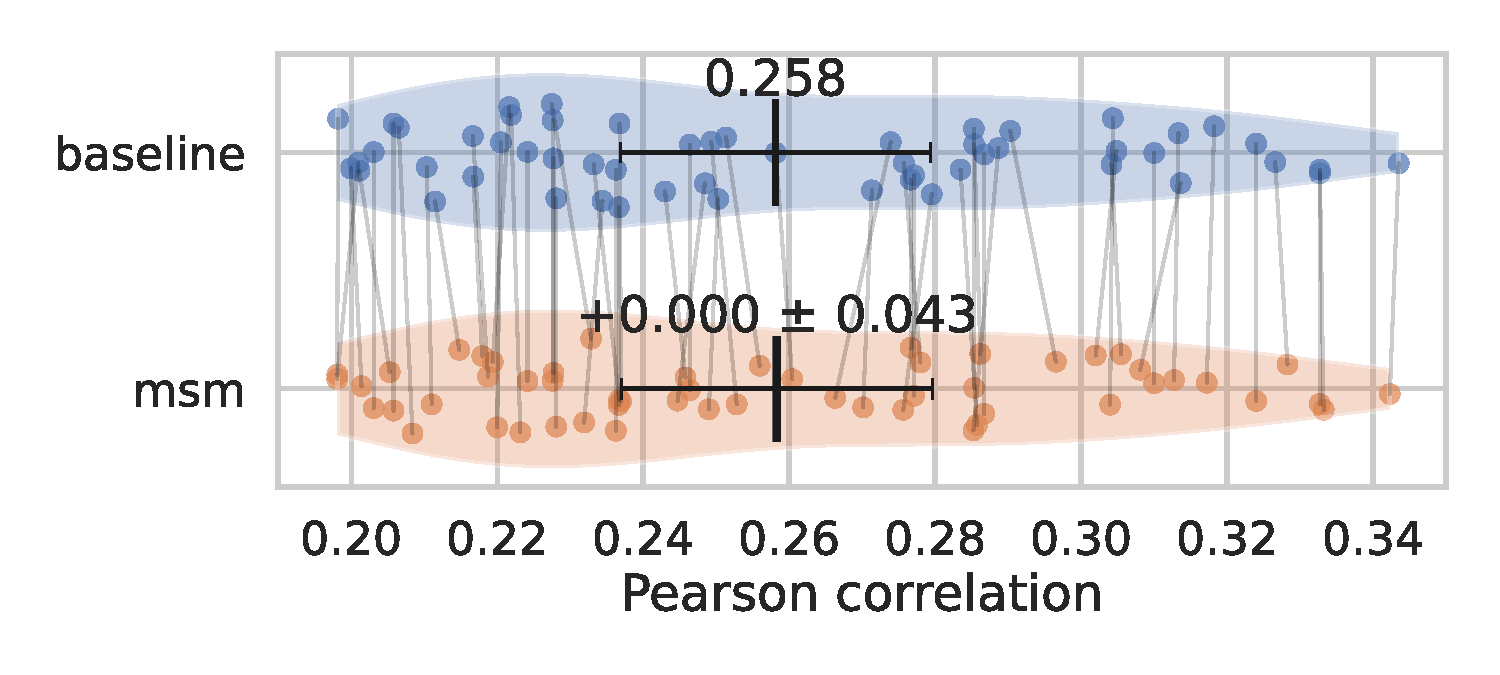
\includegraphics[width=0.49\linewidth, keepaspectratio=true]{OT_new/fsaverage5_alignment_correlation_gain_msm.pdf}
  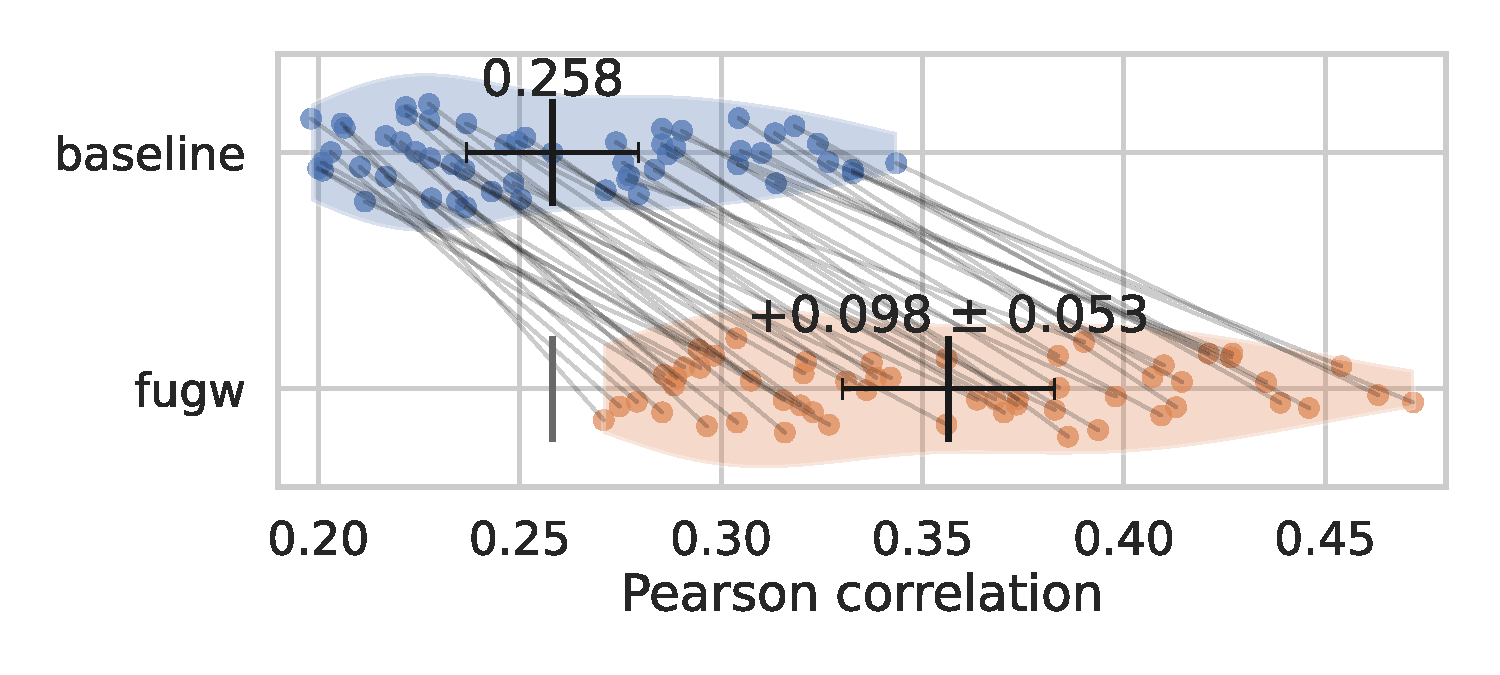
\includegraphics[width=0.49\linewidth, keepaspectratio=true]{OT_new/fsaverage5_alignment_correlation_gain_fugw.pdf}
  \caption*{\scriptsize{Comparison of gains in correlation after inter-subject alignment.}}
\end{figure}

\vspace{-0.2cm}
\begin{figure}
  \centering
  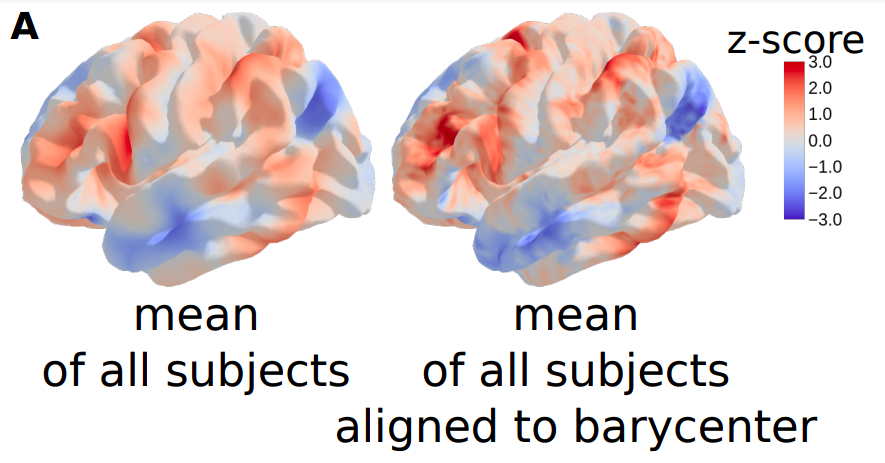
\includegraphics[width=0.4\linewidth, keepaspectratio=true]{OT_new/brain_template.png}
  \caption*{\scriptsize{FUGW barycenter yields much finer-grained maps than group averages.}}
\end{figure}

\begin{tikzpicture}[remember picture, overlay]
  \node[shift={(-3.7cm,-6cm)}] at (current page.center)
  {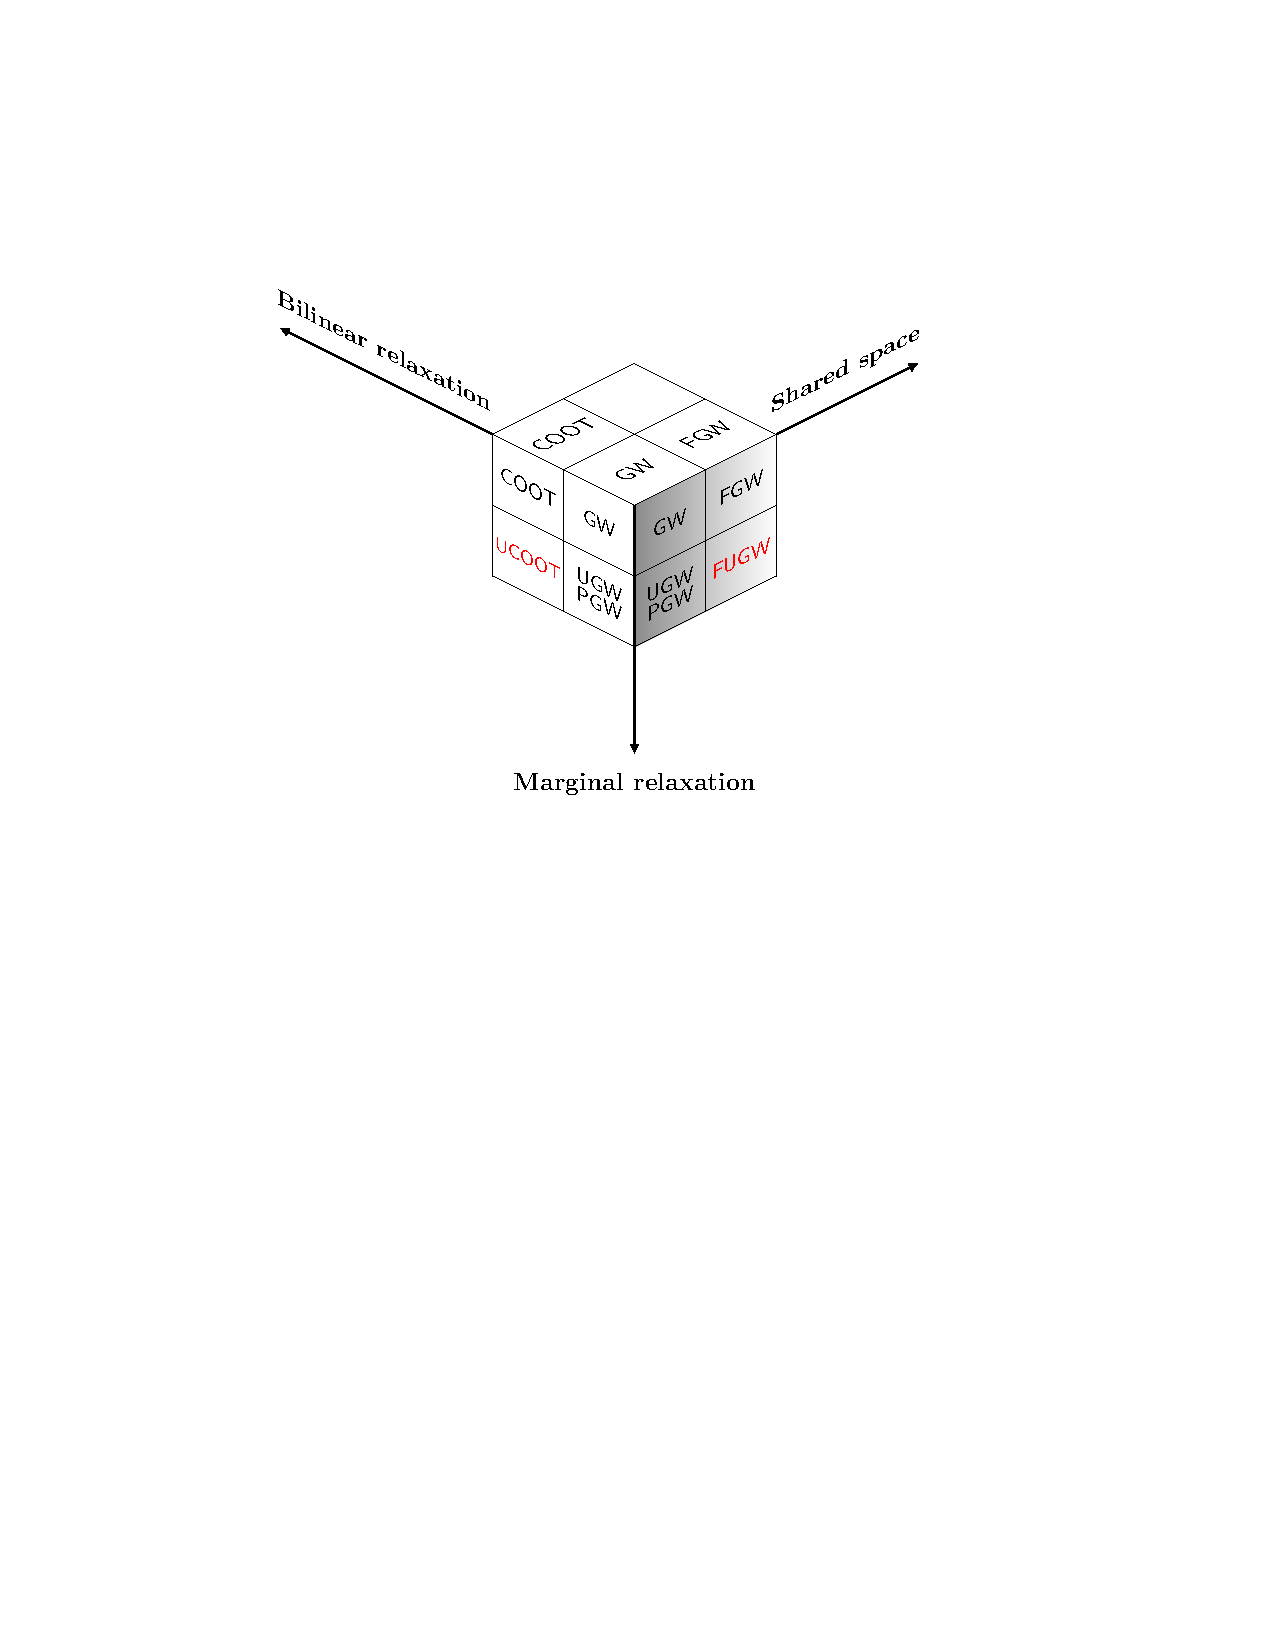
\includegraphics[scale=0.35]{OT_new/cube_fugw.pdf}};
\end{tikzpicture}

\end{frame}

%%%%%%%%%%%%%%%%%%%%%%%%%%%%%%%%%%%%%%%%%%%%%%%%%%%%%%%%%%%%%%%%%%%%%%
%%%%%%%%%%%%%%%%%%%%%%%%%%%%%%%%%%%%%%%%%%%%%%%%%%%%%%%%%%%%%%%%%%%%%%
%%%%%%%%%%%%%%%%%%%%%%%%%%%%%%%%%%%%%%%%%%%%%%%%%%%%%%%%%%%%%%%%%%%%%%
%%%% Contribution on UCOOT
\section{Unbalanced CO-Optimal Transport}

%%%%%%%%%%%%%%%%%%%%%%%%%%%%%%%%%%%%
\begin{frame}{Motivation (1)}
\scriptsize
\begin{figure}
  \centering
  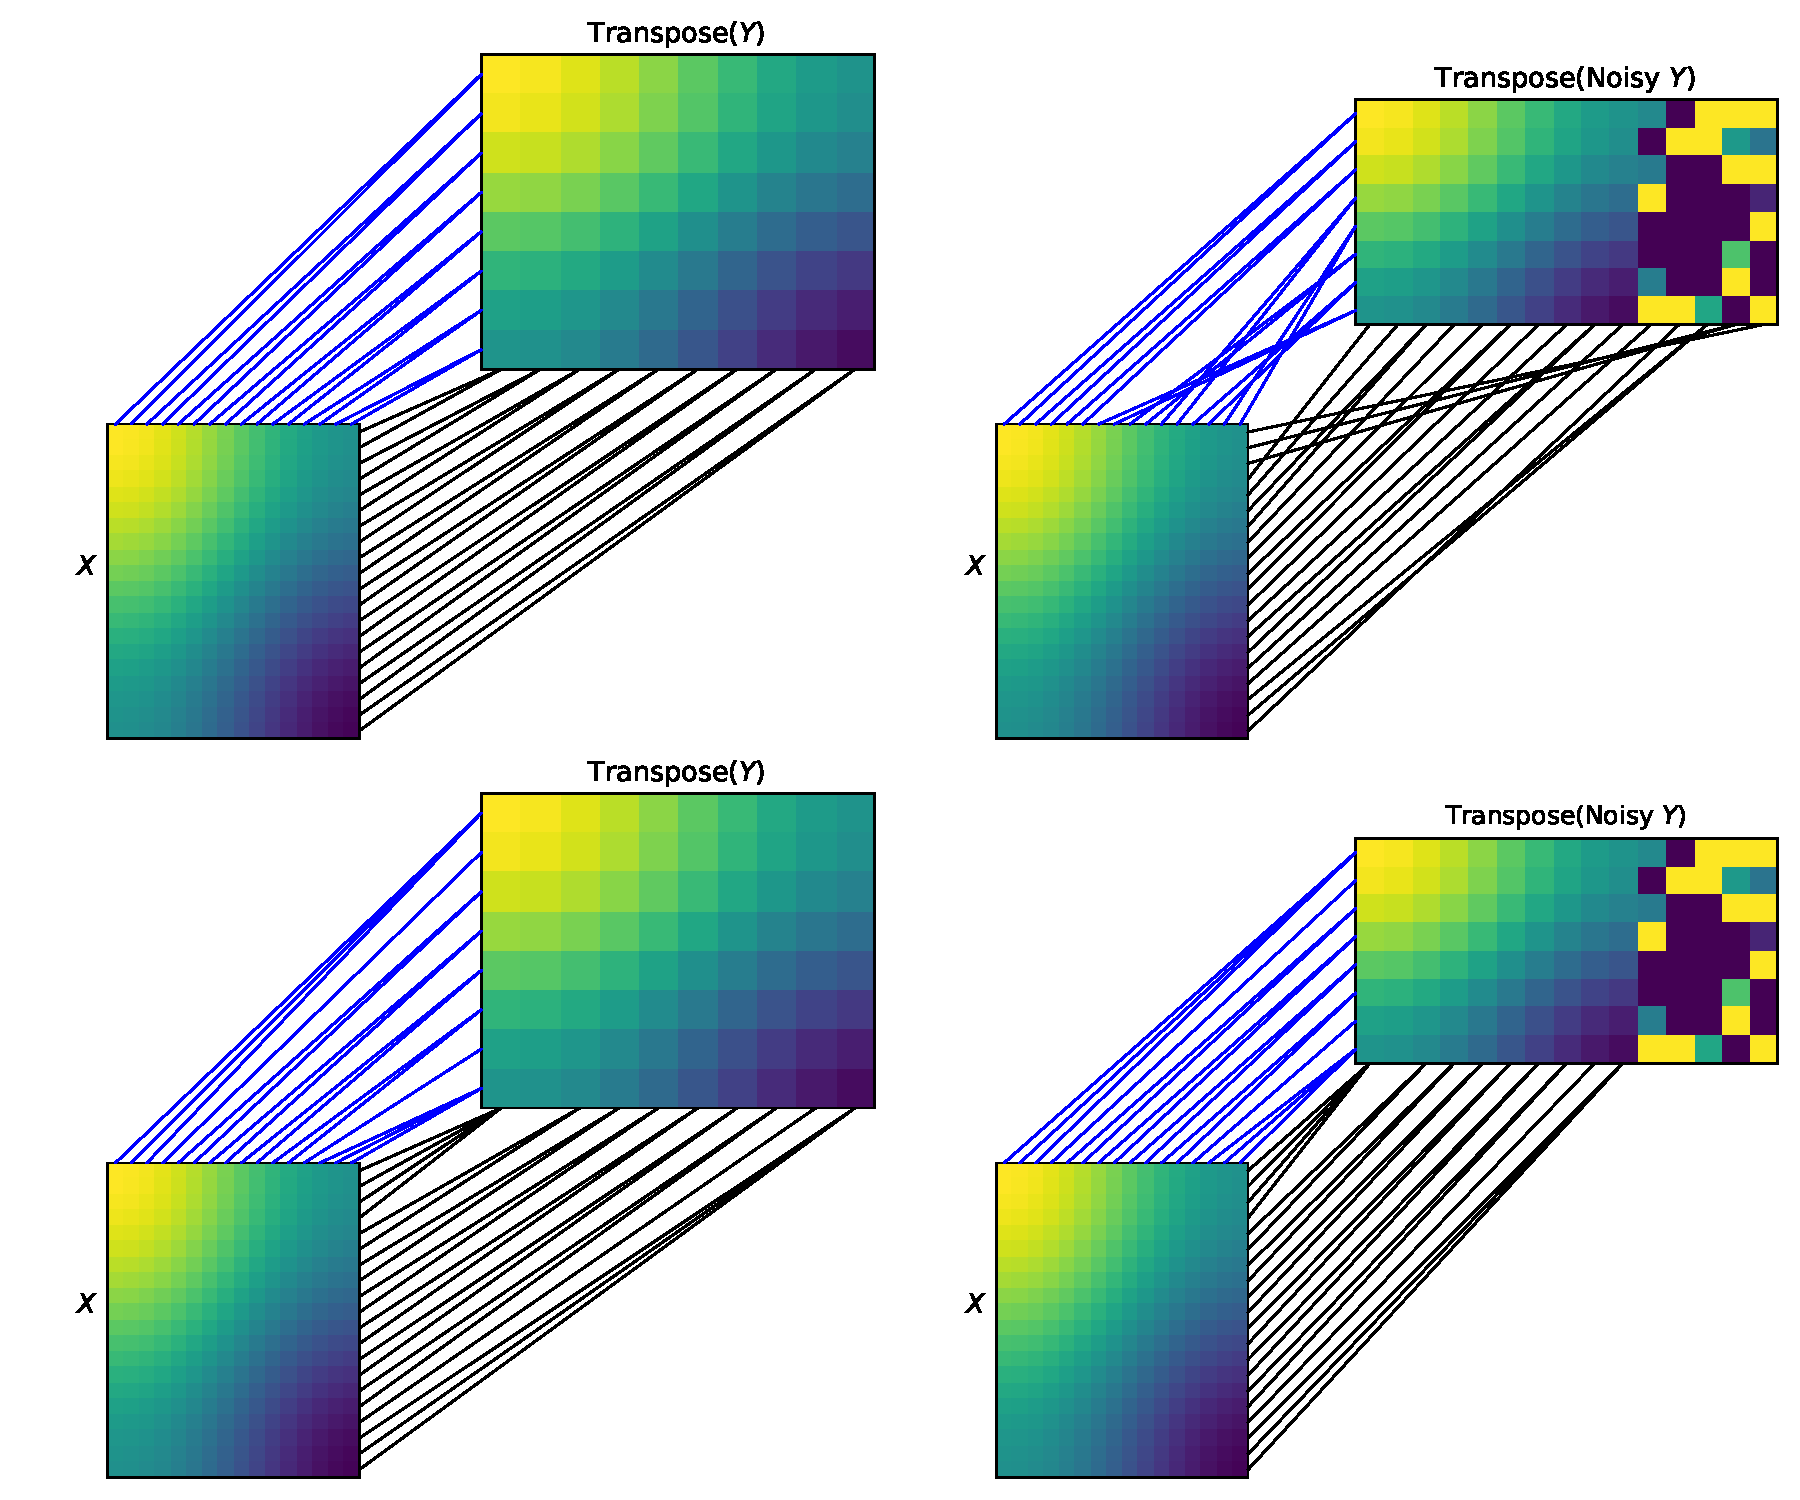
\includegraphics[width=0.9\linewidth, keepaspectratio=true]{OT_new/COOT_plot.pdf}
\end{figure}
\begin{tikzpicture}[remember picture, overlay]
  % we don't want to affect the bounding box if the rectangle is too large
  \begin{pgfinterruptboundingbox}
      % the following coords. may need to be changed to suit your slides
      \fill <1> [fill=white, opacity=0.8] (0,0) rectangle (12, 4.5);
  \end{pgfinterruptboundingbox}
  \node <1> [draw, shape=rectangle, align=right] at (10, 5.3) {%
      Hello from outliers
  };
\end{tikzpicture}
\end{frame}

%%%%%%%%%%%%%%%%%%%%%%%%%%%%%%%%%%%%
\begin{frame}{Motivation (2)}
  \scriptsize
  \begin{figure}
    \centering
    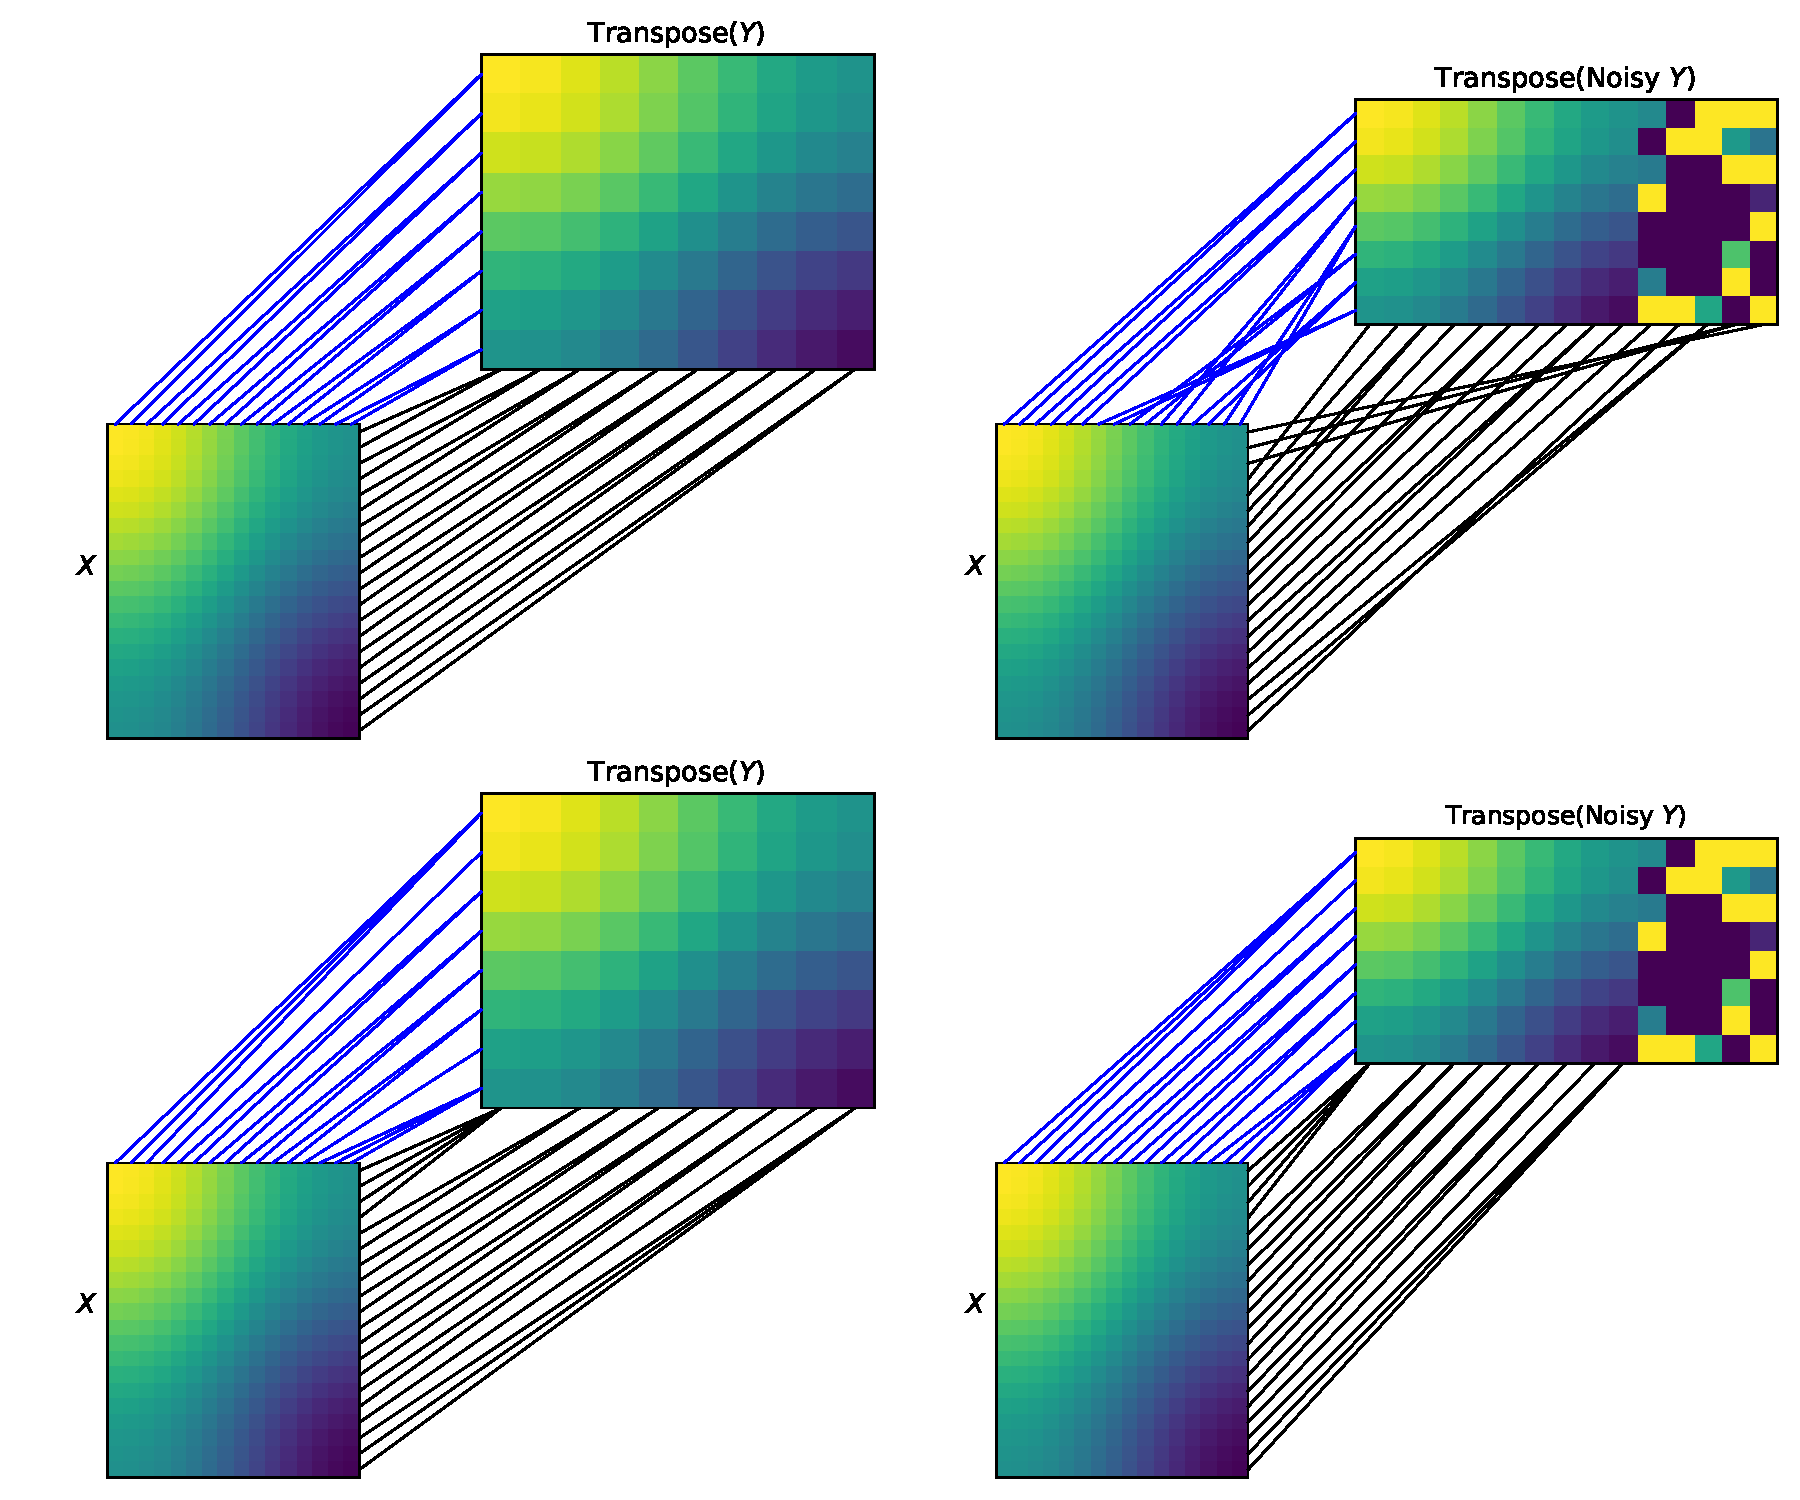
\includegraphics[width=0.9\linewidth, keepaspectratio=true]{OT_new/COOT_plot.pdf}
  \end{figure}
  \begin{tikzpicture}[remember picture, overlay]
    % we don't want to affect the bounding box if the rectangle is too large
    \begin{pgfinterruptboundingbox}
        % the following coords. may need to be changed to suit your slides
        \fill <1> [fill=white, opacity=0.8] (0,4.57) rectangle (12, 8.7);
    \end{pgfinterruptboundingbox}
    \node <1> [draw, shape=rectangle, align=right] at (10.2, 1.6) {%
        Good bye outliers
    };
  \end{tikzpicture}
\end{frame}

%%%%%%%%%%%%%%%%%%%%%%%%%%%%%%%%%%%%%%%%%%%
\begin{frame}{Summary of contributions}
  \scriptsize

  \begin{tikzpicture}[remember picture, overlay]
    \node[shift={(0cm,-1.5cm)}] at (current page.center)
    {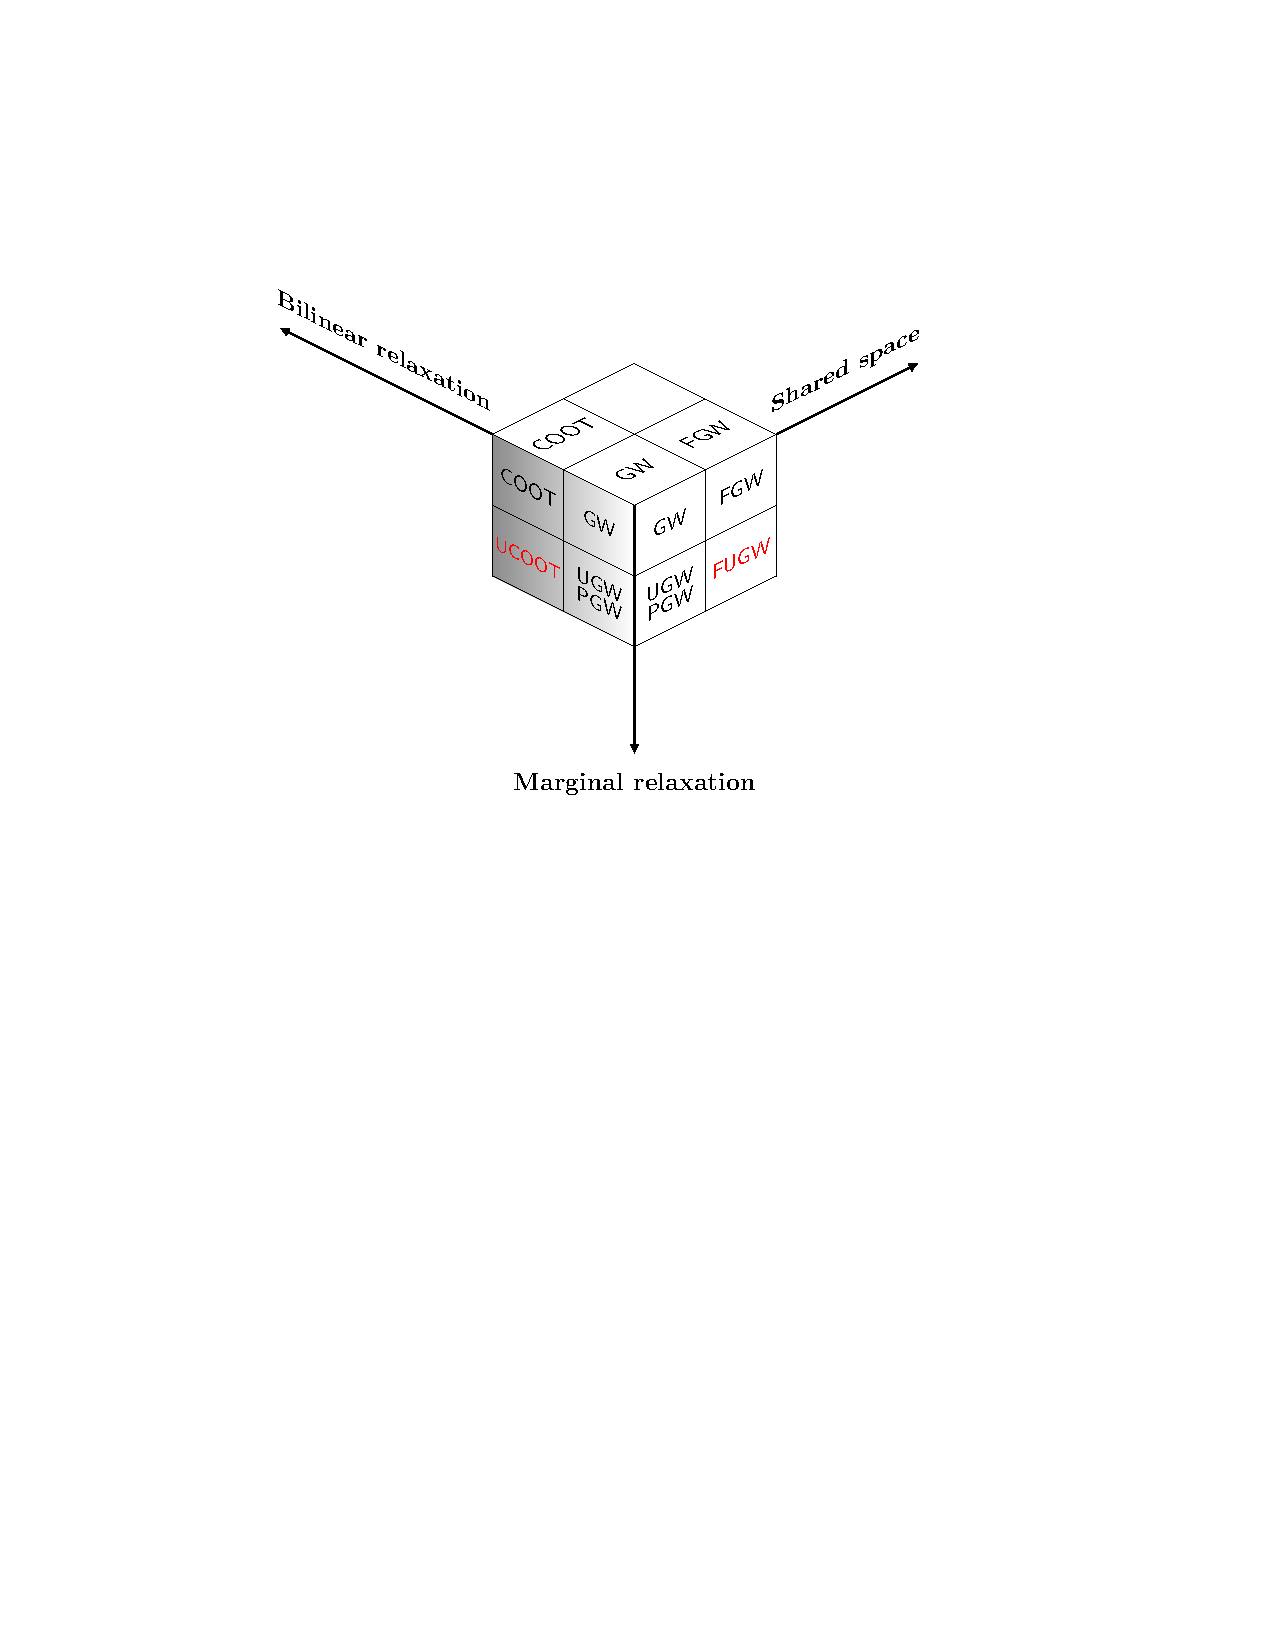
\includegraphics[scale=0.55]{OT_new/cube_ucoot_contrib.pdf}};
  \end{tikzpicture}

  \vspace{5cm}
  {\color{brown}{\textbf{Summary}}}:
  \begin{enumerate}
    \item Unbalanced formulation of COOT which is provably robust to outliers.
    \item Applications to heterogeneous domain adaptation and single-cell multi-omics.
  \end{enumerate}

  \vspace{0.3cm}
  {\color{brown}{\textbf{Publication}}}: \ul{Unbalanced Co-Optimal Transport}.
  \textbf{QHT}, Hicham Janati, Nicolas Courty, Rémi Flamary, Ievgen Redko,
  Pinar Demetci, and Ritambhara Singh.
  \textit{AAAI Conference on Artificial Intelligence}, 2023.

\end{frame}

%%%%%%%%%%%%%%%%%%%%%%%%%%%%%%%%%%%%
\begin{frame}{Unbalanced CO-Optimal Transport (1)}
\scriptsize
  \begin{definition}[{\color{blue}{Sample}} - {\color{red}{feature}} space]
    Let ${\color{blue}{(X^s, \mu^s)}}$ and ${\color{red}{(X^f, \mu^f)}}$ be compact measure spaces, where ${\color{blue}{\mu^s \in \cM^+(X^s)}}$ and ${\color{red}{\mu^f \in \cM^+(X^f)}}$. Let $\xi$ be a scalar integrable function in $L^p({\color{blue}{X^s}} \times {\color{red}{X^f}}, {\color{blue}{\mu^s}} \otimes {\color{red}{\mu^f}})$, for some $p \geq 1$. We call
    \begin{itemize}
      \item The triplet
      $\cX = \left({\color{blue}{(X^s, \mu^s)}}, {\color{red}{(X^f, \mu^f)}}, \xi \right)$
      a \underline{\textit{{\color{blue}{sample}} - {\color{red}{feature}} space}}
      (\sfspace space).

      \item The function $\xi$ an \textit{\underline{interaction}}.
    \end{itemize}
  \end{definition}
  \vspace{-0.2cm}

  \begin{tikzpicture}[remember picture, overlay]
    \node[shift={(-3.7cm,-6cm)}] at (current page.center)
    {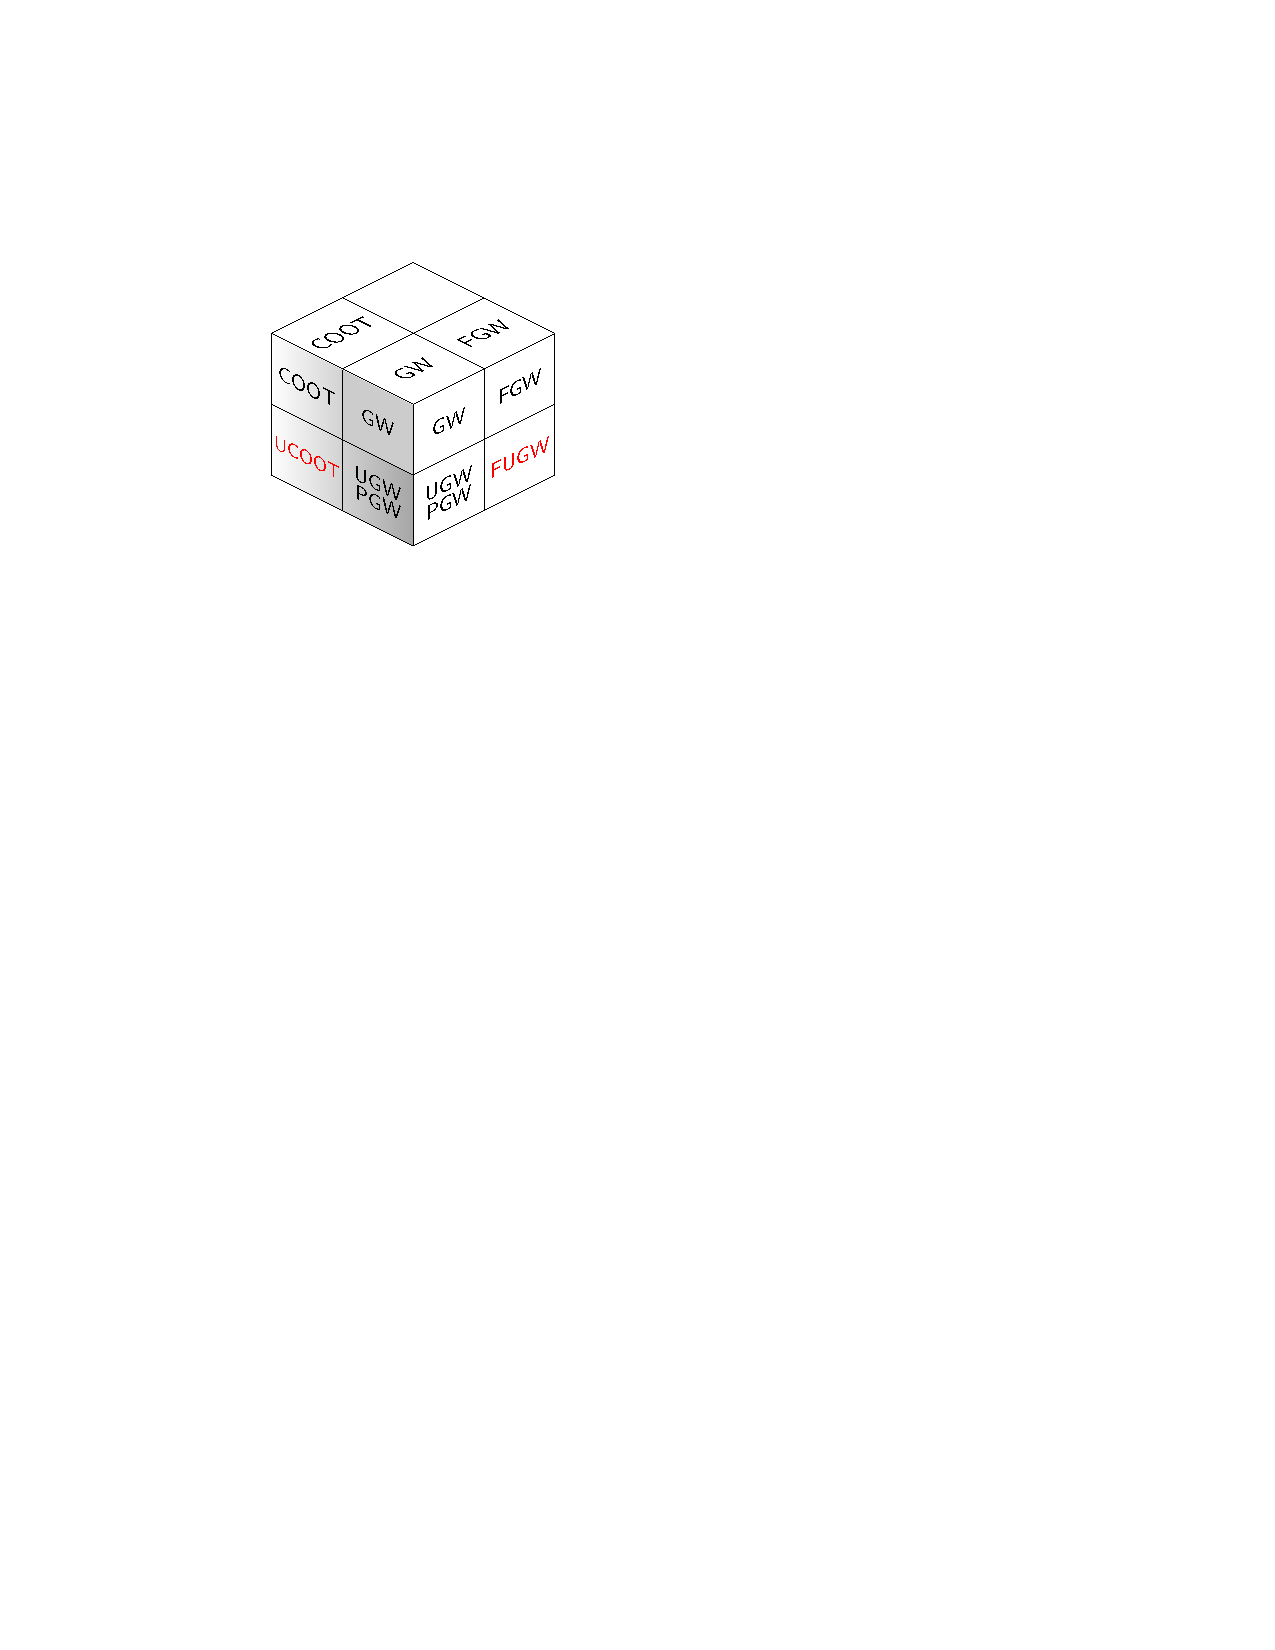
\includegraphics[scale=0.35]{OT_new/cube_ucoot.pdf}};
  \end{tikzpicture}

  \vspace{-0.3cm}
  \begin{minipage}[t]{0.6\linewidth}
  \end{minipage}%
  \hfill%
  \begin{minipage}[t]{0.8\linewidth}
  \begin{figure}
    \centering
    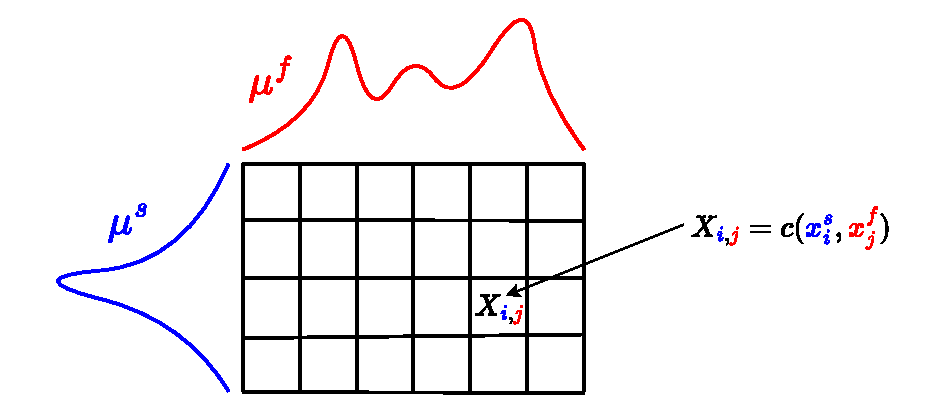
\includegraphics[width=\linewidth, keepaspectratio=true]{OT_new/coot_matrix_single.pdf}
  \end{figure}
  \end{minipage}

\end{frame}

%%%%%%%%%%%%%%%%%%%%%%%%%%%%%%%%%%%%%%%%%%%%%%%%%%%
\begin{frame}{Unbalanced CO-Optimal Transport (2)}
\scriptsize
\vspace{-1cm}
\begin{definition}[UCOOT]
    Given $\lambda_1, \lambda_2 >0$, the unbalanced COOT of order $p \geq 1$
    between two \sfspace spaces $\cX_1 = \left({\color{blue}{(X_1^s, \mu_1^s)}}, {\color{red}{(X_1^f, \mu_1^f)}}, \xi_1 \right)$
    and $\cX_2 = \left({\color{blue}{(X_2^s, \mu_2^s)}}, {\color{red}{(X_2^f, \mu_2^f)}}, \xi_2 \right)$ is defined by
\begin{align*}
\label{eq:ucoot}
    \ucoot_{\lambda}(\cX_1, \cX_2) :=
  \inf_{\substack{{\color{blue}{\pi^s \in \cM^+(X_1^s \times X_2^s)}}
  \\ {\color{red}{\pi^f \in \cM^+(X_1^f \times X_2^f)}}}}
  \cL_{\ucoot}(\pis, \pif).
\end{align*}
\vspace{-0.8cm}
where:
\begin{align*}
    \cL_{\ucoot}(\pis, \pif) &= \underbrace{\iint
    |\xi_1({\color{blue}{x_1^s}}, {\color{red}{x_1^f}}) - \xi_2({\color{blue}{x_2^s}}, {\color{red}{x_2^f}})|^p \; {\color{blue}{\mathrm d\pi^s(x_1^s, x_2^s)}} \;
    {\color{red}{\mathrm d \pi^f(x_1^f, x_2^f)}}}_{\text{transport cost of {\color{blue}{sample}}-{\color{red}{feature}} pairs}} \\
    &+ \underbrace{\sum_{k=1}^2\lambda_k \; \text{KL}({\color{blue}{\pi^s_{\# k}}} \otimes {\color{red}{\pi^f_{\# k}}} \vert {\color{blue}{\mu^s_k}} \otimes {\color{red}{\mu^f_k}})}_{\text{mass destruction / creation penalty}}.
\end{align*}
\end{definition}

\begin{tikzpicture}[remember picture, overlay]
  \node[shift={(-3.7cm,-6cm)}] at (current page.center)
  {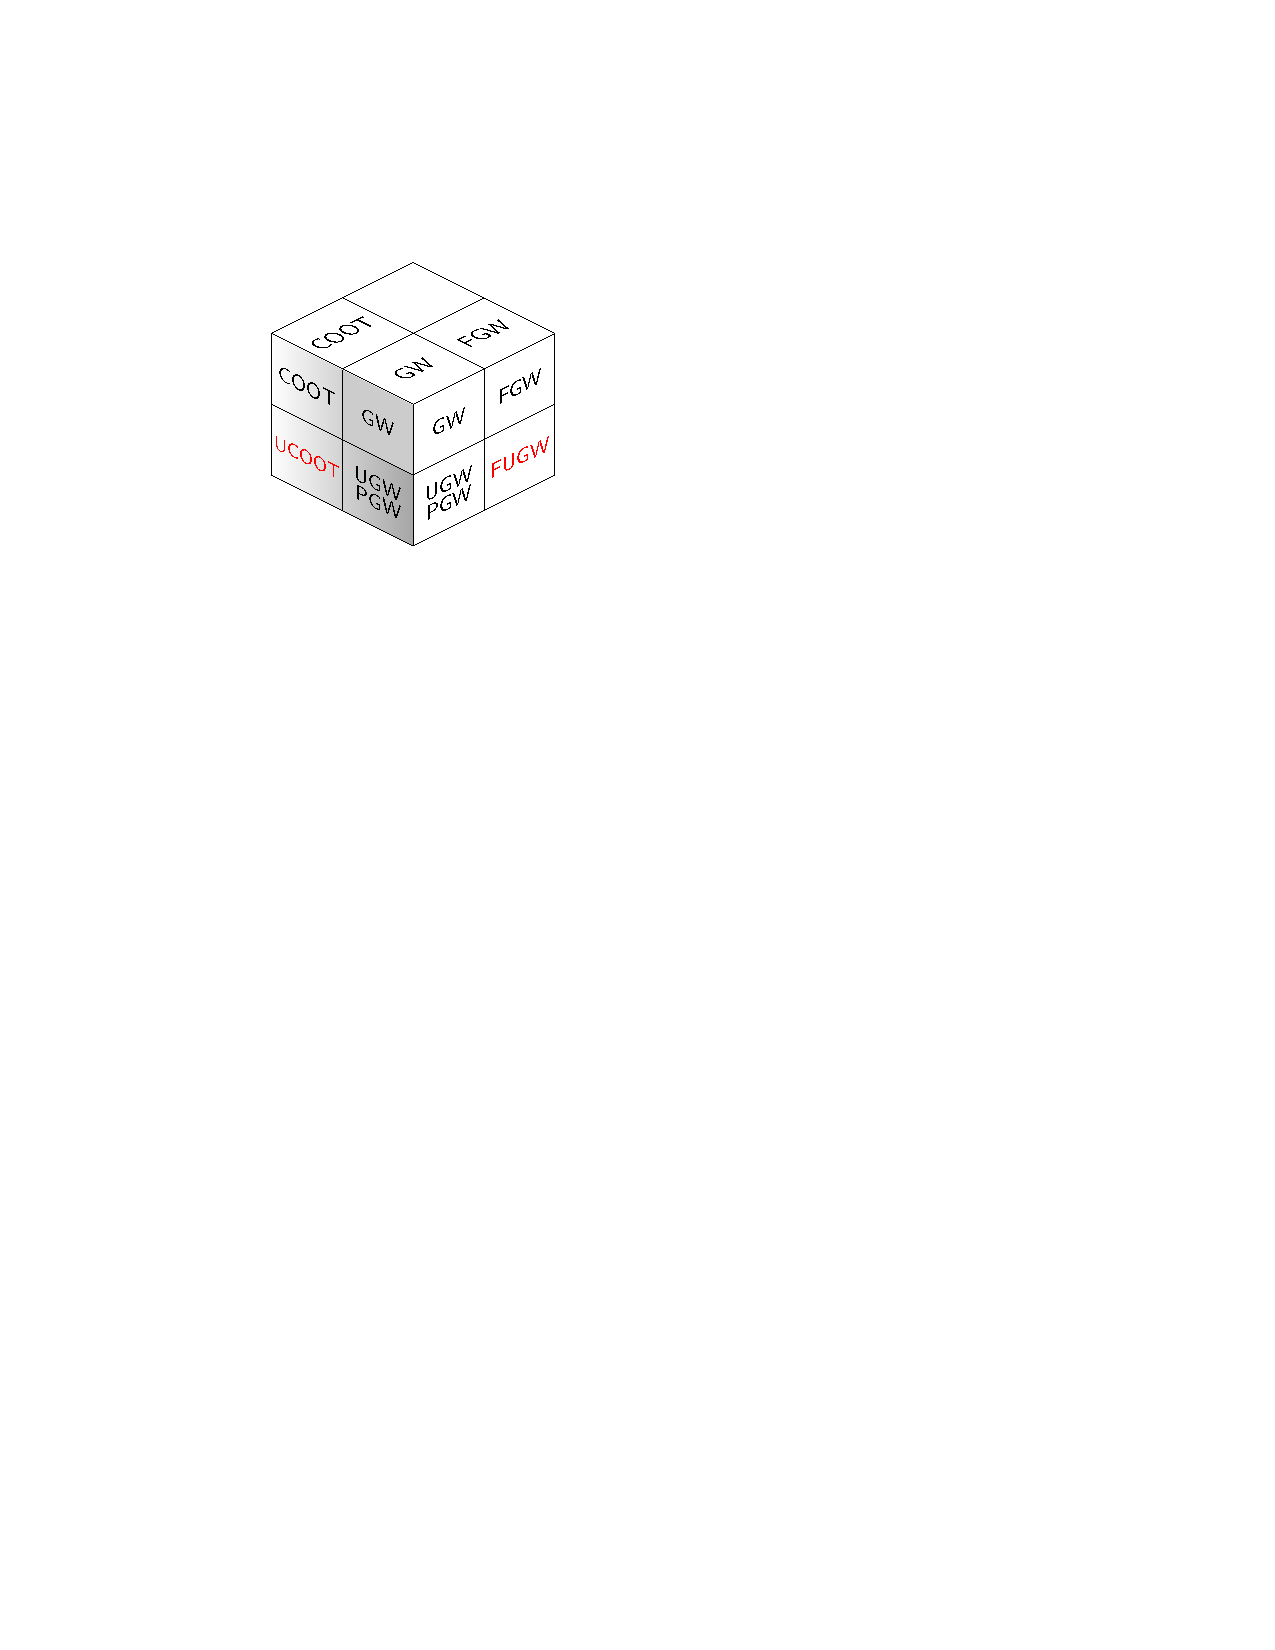
\includegraphics[scale=0.35]{OT_new/cube_ucoot.pdf}};
\end{tikzpicture}

\end{frame}

%%%%%%%%%%%%%%%%%%%%%%%%%
\begin{frame}{Provable robustness of UCOOT (1)}
\scriptsize
  \begin{definition}[Noisy \sfspace space]
  Given two \textbf{clean} \sfspace spaces
  $\cX_1 = \left({\color{blue}{(X_1^s, \mu_1^s)}}, {\color{red}{(X_1^f, \mu_1^f)}}, \xi_1 \right),
  \cX_2 = \left({\color{blue}{(X_2^s, \mu_2^s)}}, {\color{red}{(X_2^f, \mu_2^f)}}, \xi_2 \right)$.
  \begin{enumerate}
      \item \textbf{Noisy} \sfspace space: $\widetilde{\cX_1} = \left( {\color{blue}{(X^s_1 \cup O^s, \widetilde{\mu}^s_1)}}, {\color{red}{(X^f_1 \cup O^f, \widetilde{\mu}^f_1)}}, \xi_1 \right)$, where
      \begin{itemize}
        \scriptsize
          \item {\color{blue}{\textbf{Noisy} measure on sample space:
          $\widetilde{\mu}^s_1 = \alpha_s \mu^s_1 + (1-\alpha_s) \varepsilon^s$, for $\alpha_s \in [0,1], \varepsilon^s \in \cM^+(O^s)$.}}
          \item {\color{red}{\textbf{Noisy} measure on feature space: $\widetilde{\mu}^f_1 = \alpha_f \mu^f_1 + (1-\alpha_f) \varepsilon^f$, for $\alpha_f \in [0,1], \varepsilon^f \in \cM^+(O^f)$.}}
      \end{itemize}

      \item Minimal cost: $\Delta_{0} := \min_{\substack{
        {\color{blue}{x_1^s \in O^s}}, {\color{red}{x_1^f \in O^f}} \\
        {\color{blue}{x_2^s \in X_2^s}}, {\color{red}{x_2^f \in X_2^f}}}}\quad \left| \xi_1({\color{blue}{x_1^s}}, {\color{red}{x_1^f}}) - \xi_2({\color{blue}{x_2^s}}, {\color{red}{x_2^f}}) \right|^p$.

    \item Maximal cost: $\Delta_{\infty} := \max_{
    \substack{
    {\color{blue}{x_1^s \in X_1^s \cup O^s}}, {\color{red}{x_1^f \in X_1^f \cup O^f}} \\
    {\color{blue}{x_2^s \in X_2^s}}, {\color{red}{x_2^f \in X_2^f}}
    }} \quad \left| \xi_1({\color{blue}{x_1^s}}, {\color{red}{x_1^f}}) - \xi_2({\color{blue}{x_2^s}}, {\color{red}{x_2^f}}) \right|^p$.
  \end{enumerate}
  \end{definition}
  $\Rightarrow$ Both costs can explode if the outliers are too impactful.

  \begin{tikzpicture}[remember picture, overlay]
    \node[shift={(-3.7cm,-6cm)}] at (current page.center)
    {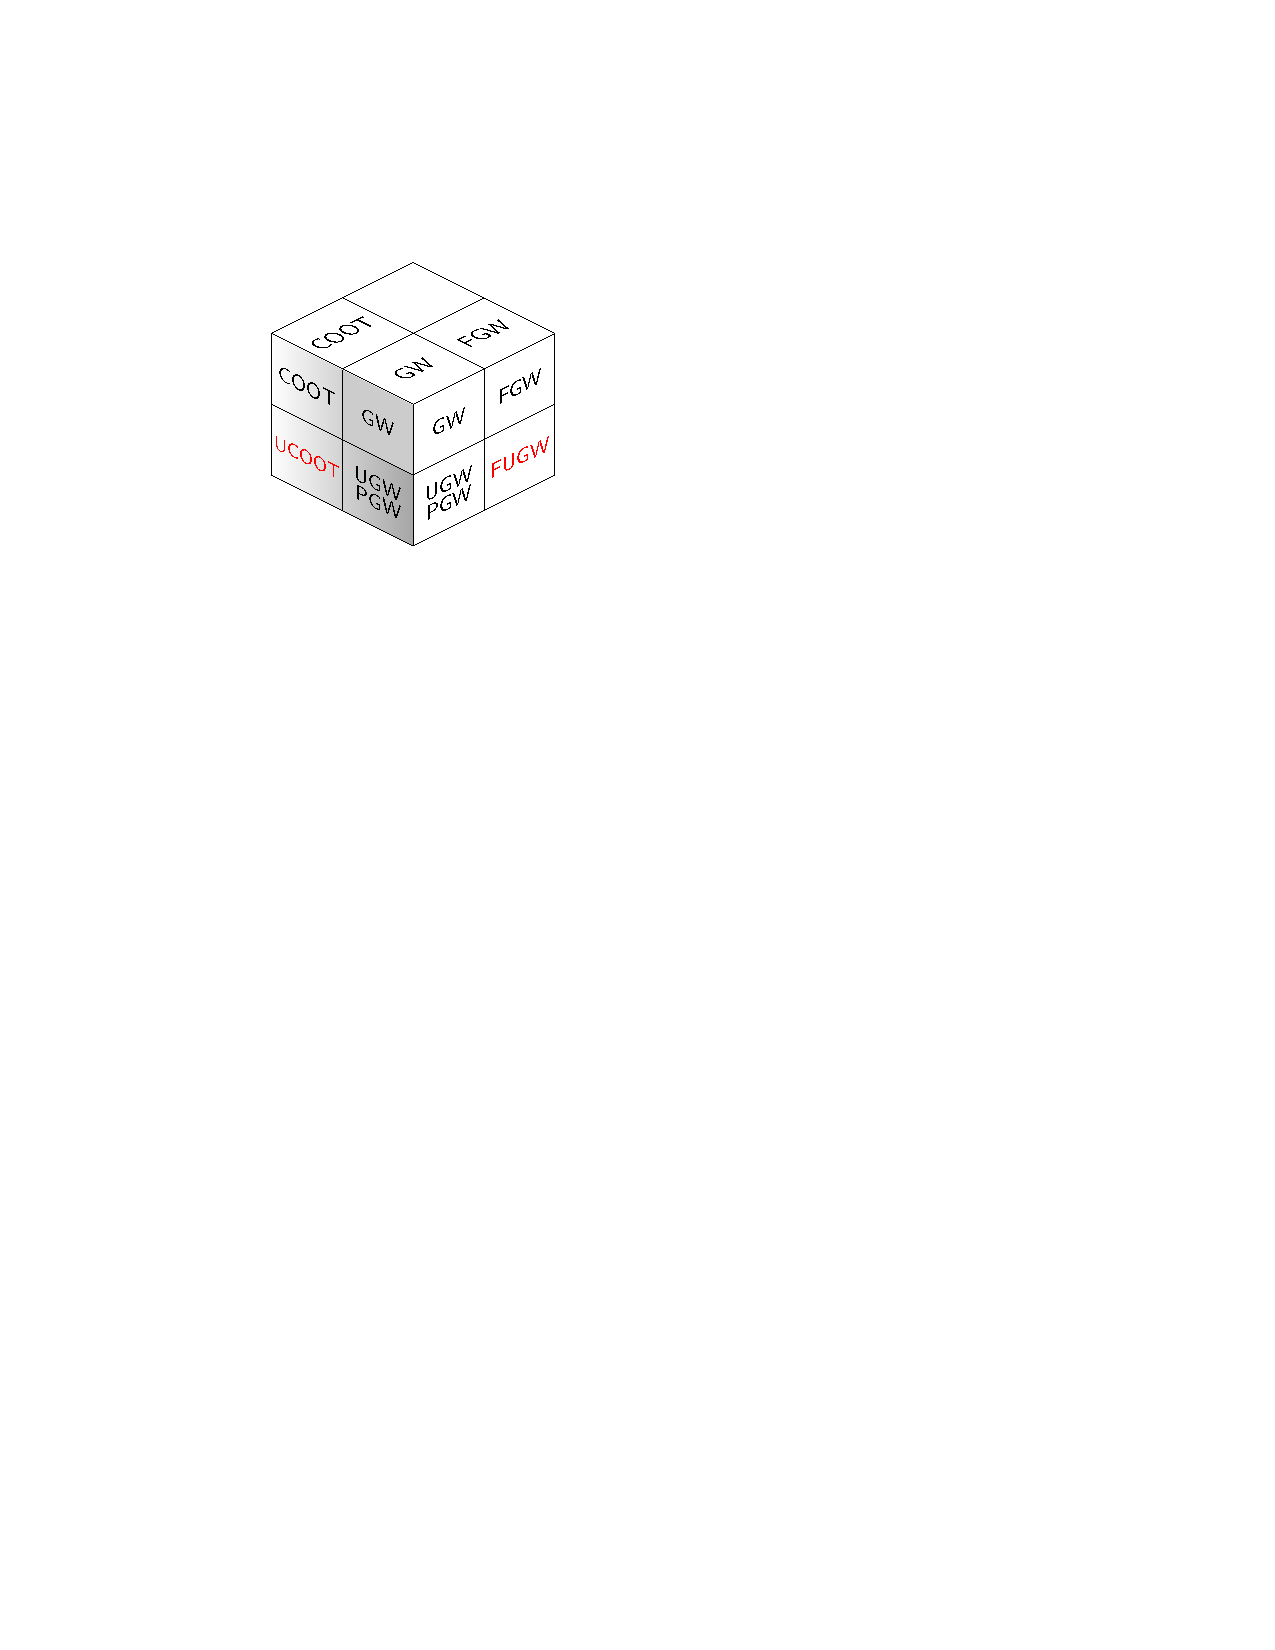
\includegraphics[scale=0.35]{OT_new/cube_ucoot.pdf}};
  \end{tikzpicture}

\end{frame}

\begin{frame}{Provable robustness of UCOOT (2)}
\scriptsize
\vspace{-0.2cm}
\begin{proposition}
  \begin{enumerate}
    \setlength\itemsep{0em}
    \item COOT is sensitive to outliers:
    $\coot(\widetilde{\cX_1}, \cX_2) \geq (1 - {\color{blue}{\alpha_s}})(1 - {\color{red}{\alpha_f}})\Delta_0$.

    \item UCOOT is robust to outliers: denote
    \begin{itemize}
      \scriptsize
      \item $\delta = 2(\lambda_1 + \lambda_2)(1 - {\color{blue}{\alpha_s}} {\color{red}{\alpha_f}})$.

      \item $M= m(\pis) = m(\pif)$: mass of OT plans between clean data.

      \item $K = M + \frac{1}{M}\ucoot_{\lambda}(\cX_1, \cX_2) + \delta$.
    \end{itemize}
    \begin{equation*} %\label{eq:ucoot-robust}
    \begin{split}
      \underbrace{\ucoot_{\lambda}(\widetilde{\cX_1}, \cX_2)}_{\text{"noisy divergence"}}
      &\leq {\color{blue}{\alpha_s}} {\color{red}{\alpha_f}}
      \underbrace{\ucoot_{\lambda}(\cX_1, \cX_2)}_{\text{"clean divergence"}}
      + \underbrace{\delta M \left[ 1 -
      \exp \left( {- \frac{\Delta_{\infty}(1+M) + K}{\delta M}} \right) \right]}_{\text{saturates quickly if } \Delta_{\infty} \to \infty}.
    \end{split}
    \end{equation*}
  \end{enumerate}

  \begin{tikzpicture}[remember picture, overlay]
    \node[shift={(-3.7cm,-6cm)}] at (current page.center)
    {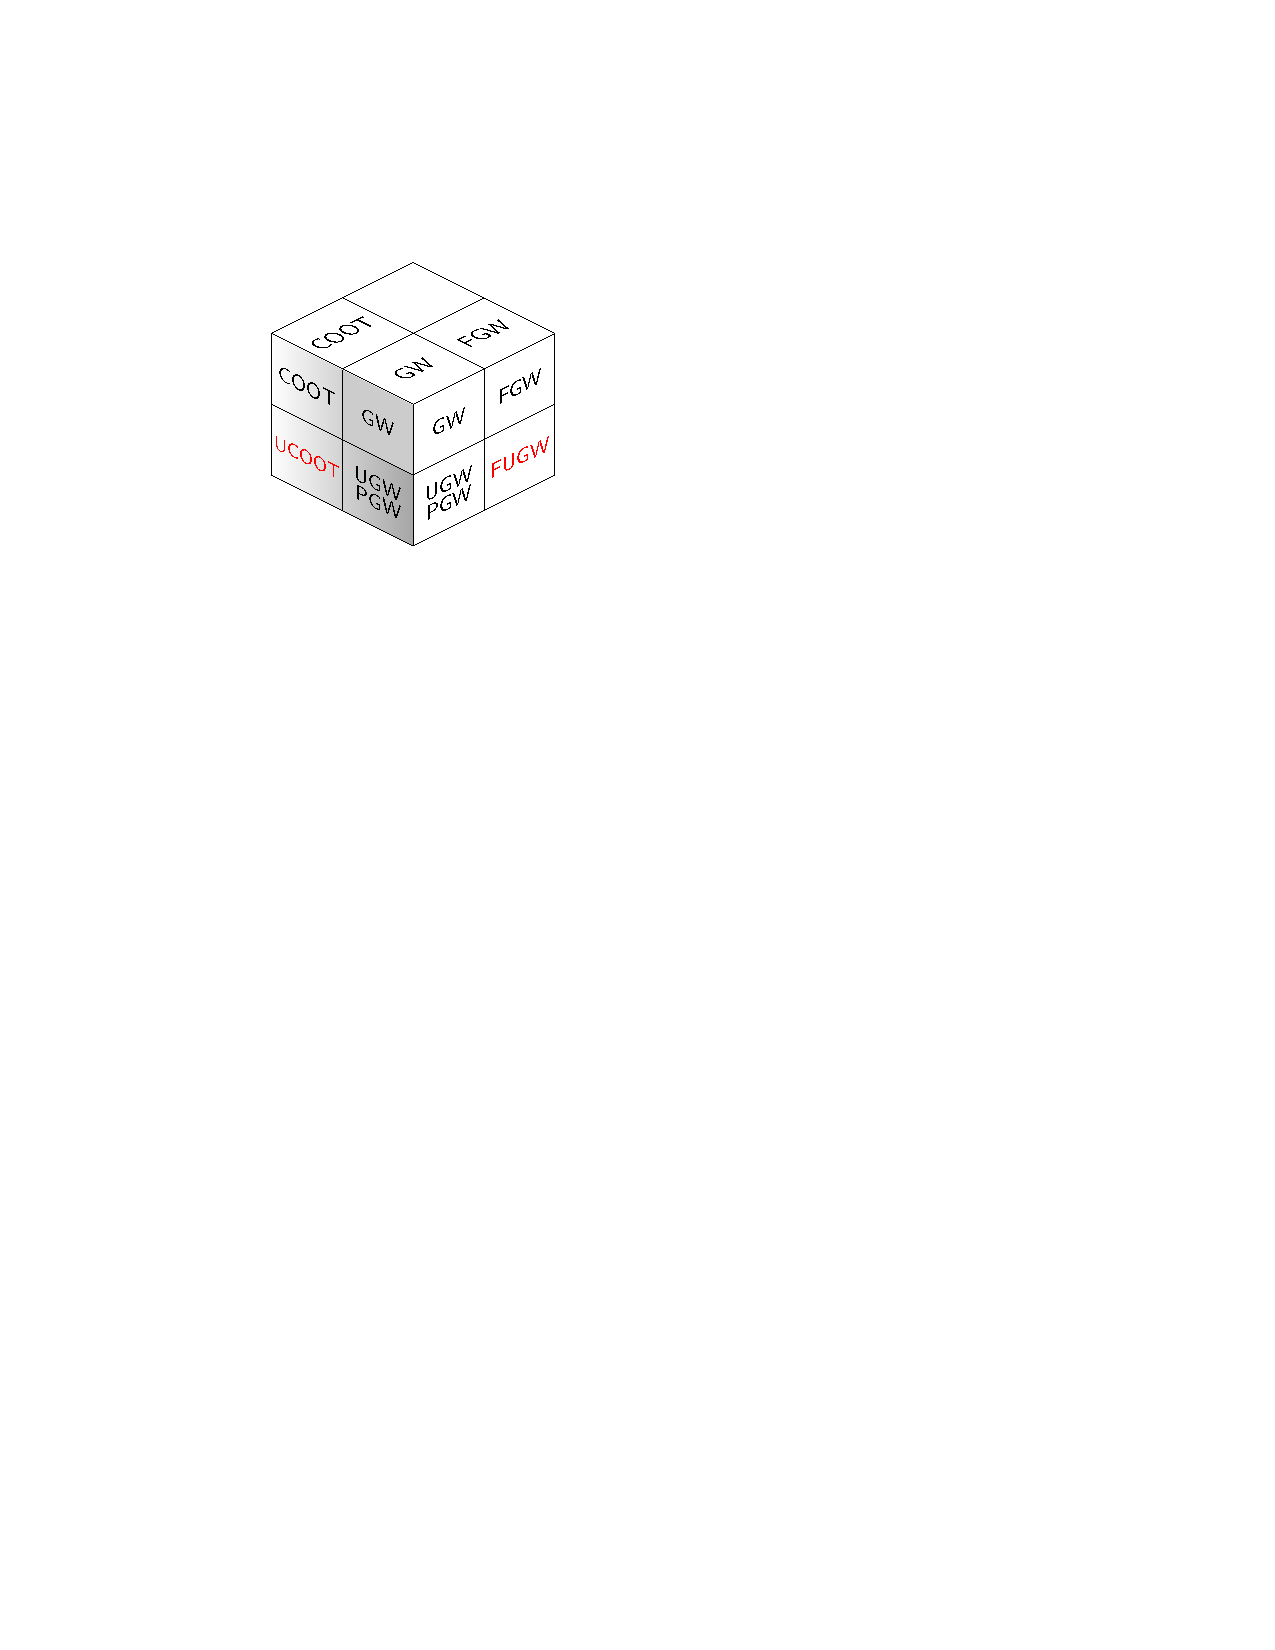
\includegraphics[scale=0.35]{OT_new/cube_ucoot.pdf}};
  \end{tikzpicture}
\end{proposition}

\begin{minipage}[t]{0.6\linewidth}
  \begin{itemize}
    \item UCOOT is always upper bounded.
    \item Robustness also holds for unbalanced GW.
  \end{itemize}
\end{minipage}%
\hfill%
\hspace{-6cm}
\begin{minipage}[t]{0.5\linewidth}
  \vspace{-0.3cm}
  \begin{figure}
    \centering
    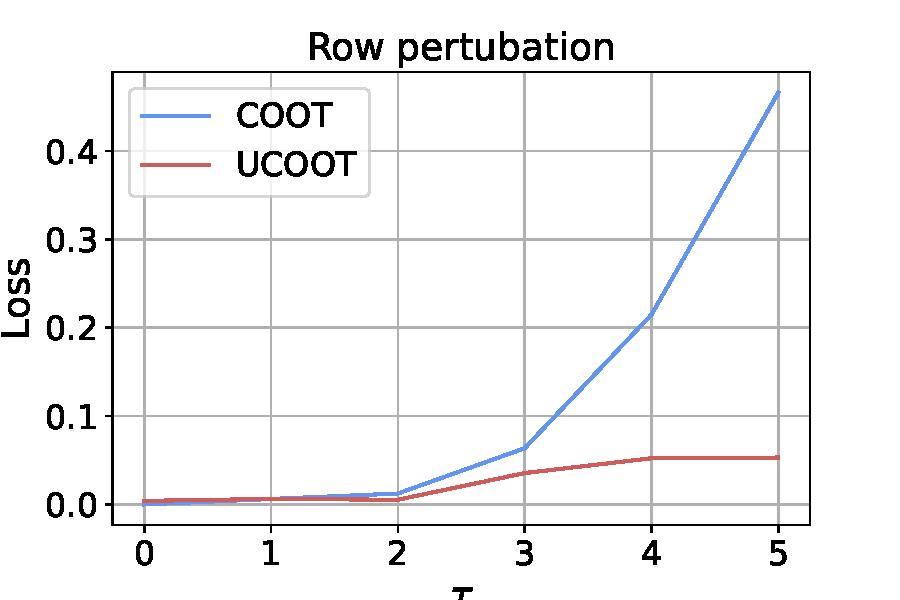
\includegraphics[width=\linewidth, keepaspectratio=true]{SIMPAS/robustness_2.pdf}
  \end{figure}
\end{minipage}

\end{frame}

%%%%%%%%%%%%%%%%%%%%%%%%%%%%%%%%%
\begin{frame}{Illustration 1: MNIST images}
\scriptsize
\begin{figure}
    \centering
    \includegraphics[width=1.05\linewidth, keepaspectratio=true]{SIMPAS/mnist-ucoot-rebuttal.pdf}
    \vspace*{-1cm}
    % \caption*{\scriptsize{Example illustrating and interpreting
    % the {\color{red}{feature alignment $\pi^f$}} learned by UCOOT
    % and its robustness to outliers.}}
\end{figure}
\end{frame}

%%%%%%%%%%%%%%%%%%%%%%%%%%%%%%%%%
\begin{frame}{Illustration 2: Single-cell multi-omics (with Pinar Demetci)}
\scriptsize
\begin{figure}
      \centering
      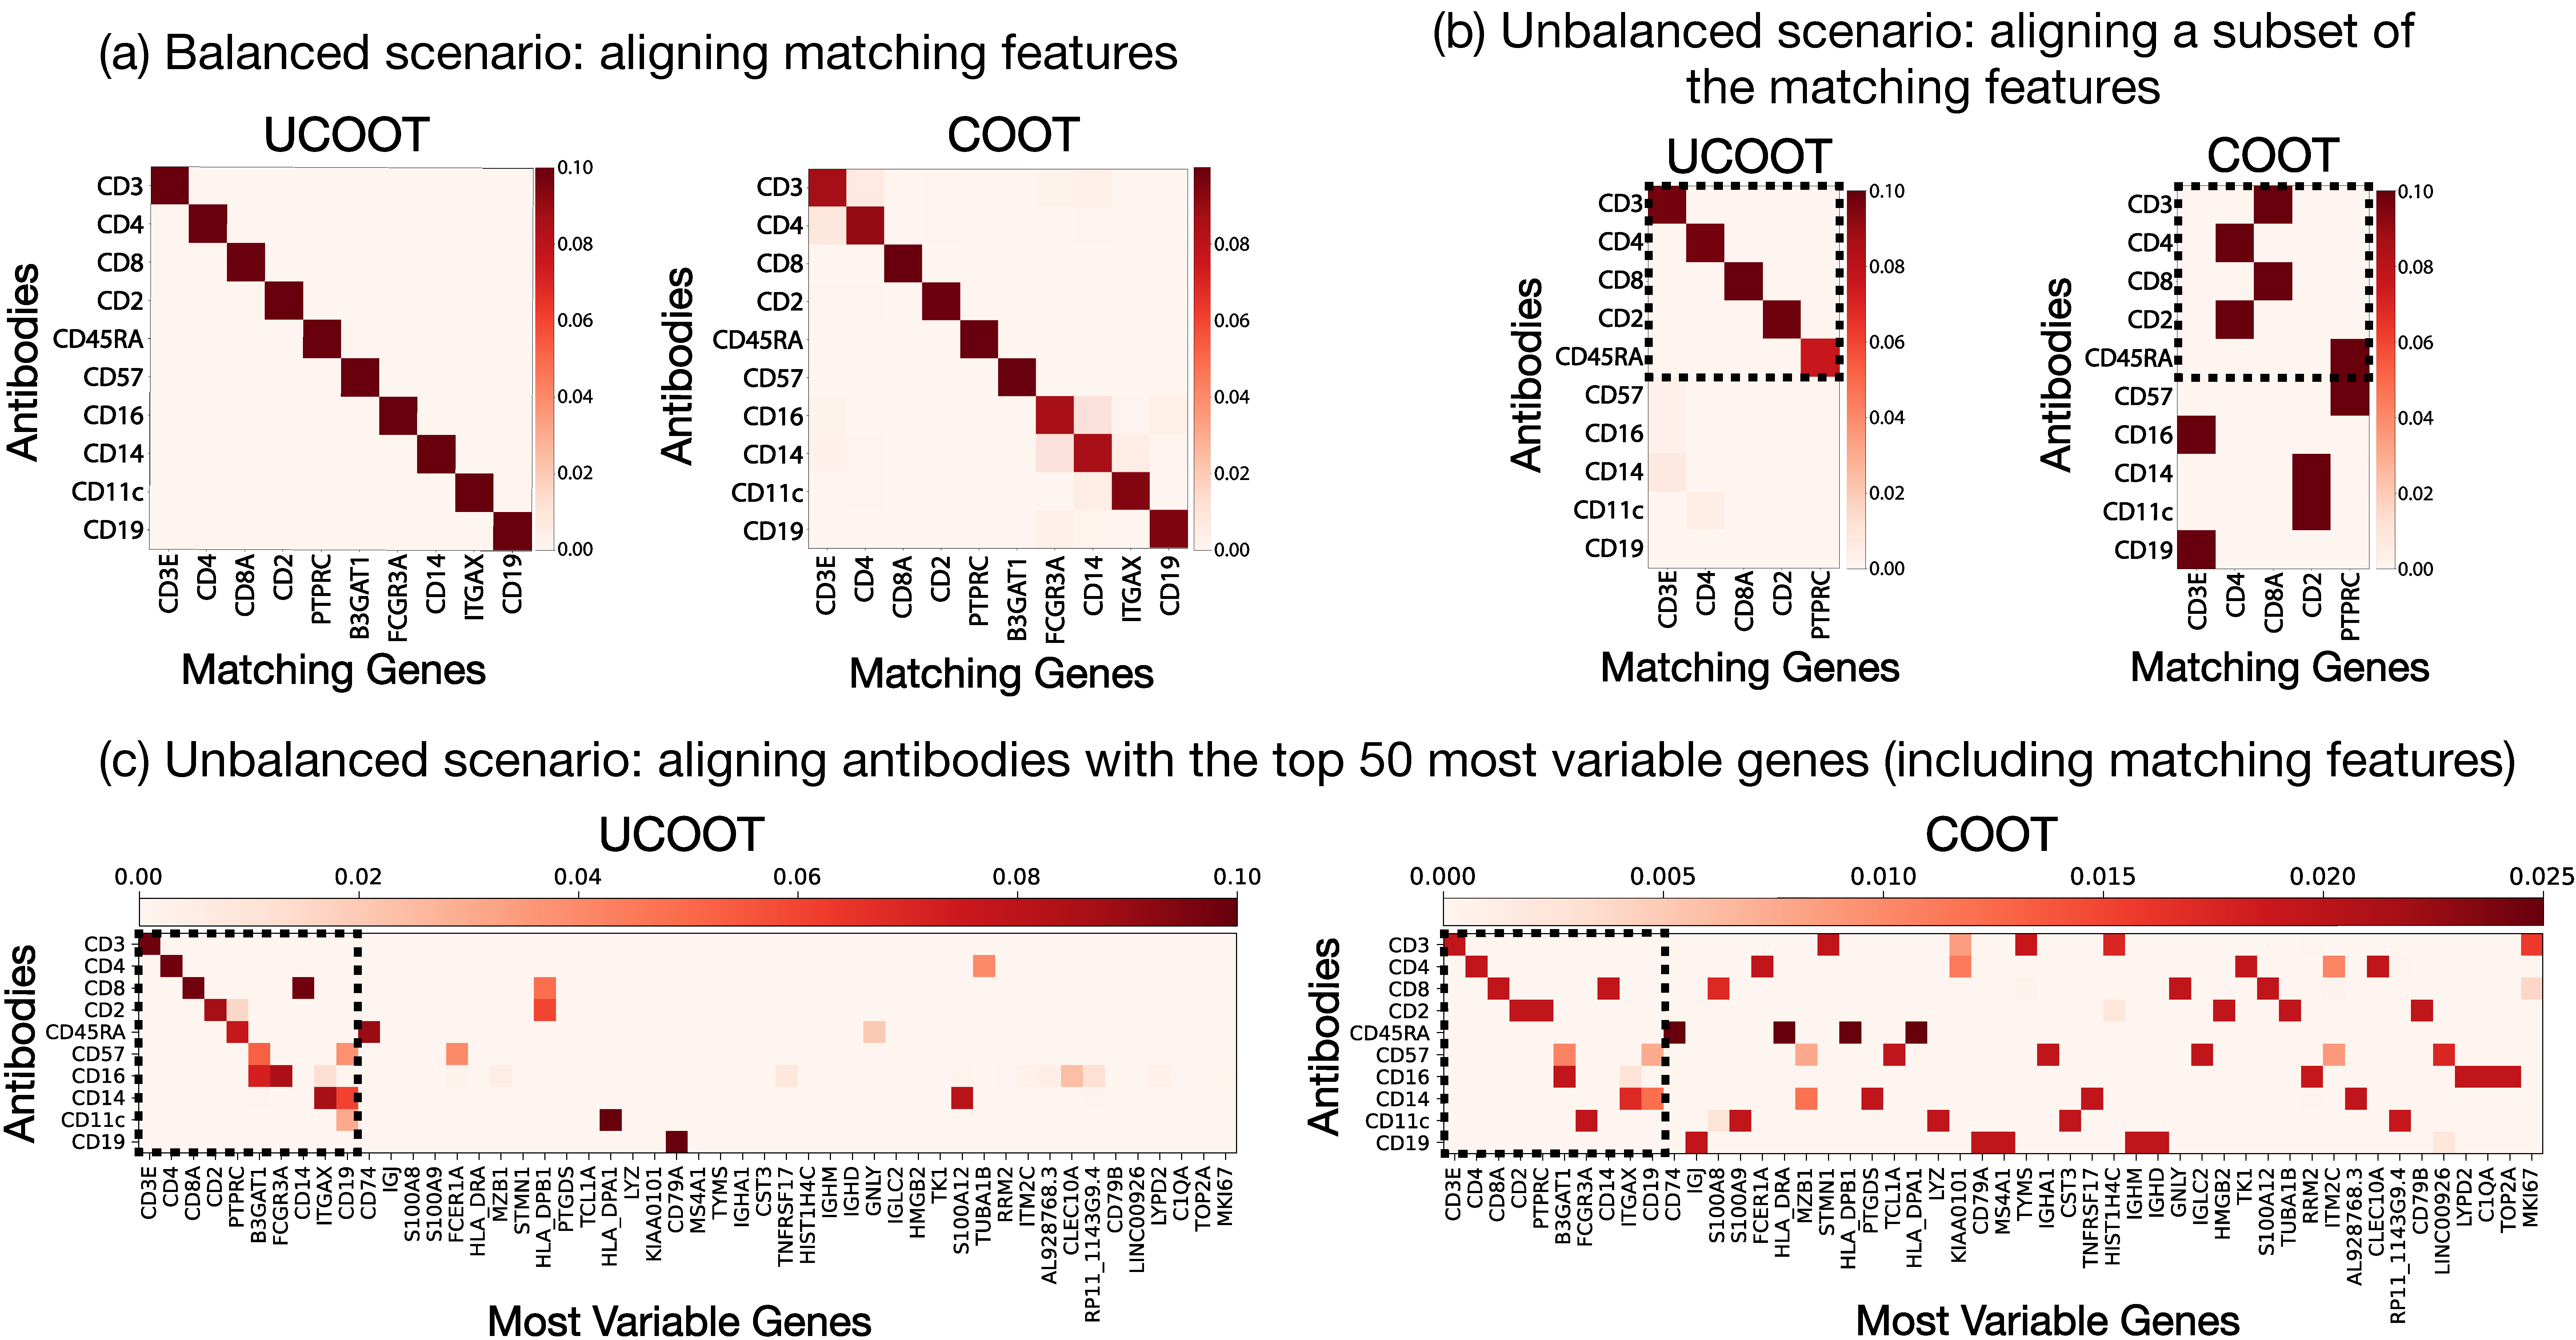
\includegraphics[width=1.05\linewidth, keepaspectratio=true]{OT_new/genes-alignments.pdf}
      % \caption*{\scriptsize{Example illustrating and interpreting the
      % {\color{red}{feature alignment $\pi^f$}} learned by UCOOT
      % and its robustness to outliers.}}
  \end{figure}
\end{frame}

%%%%%%%%%%%%%%%%%%%%%%%%%%%%%%%%%%%%%%%%%%%%%%%%%%%%%%%%%%%%%%%%%%%%%%
%%%%%%%%%%%%%%%%%%%%%%%%%%%%%%%%%%%%%%%%%%%%%%%%%%%%%%%%%%%%%%%%%%%%%%
%%%%%%%%%%%%%%%%%%%%%%%%%%%%%%%%%%%%%%%%%%%%%%%%%%%%%%%%%%%%%%%%%%%%%%
%%%% Contribution on AGW
\section{Augmented Gromov-Wasserstein}

%%%%%%%%%%%%%%%%%%%%%%%%%%%%%%%%%%%%%%
\begin{frame}{Motivation}
%%%%%%%%%%%%%%%%%%%%%%%%%%%%%%%%%
\scriptsize

\begin{enumerate}
  \item Isometries are useful for across-space comparison.
  \item All isometries are created equal, but some are more equal than others.
  \item GW induces all isometries but COOT is good at exploiting data.
\end{enumerate}
\begin{figure}
    \centering
    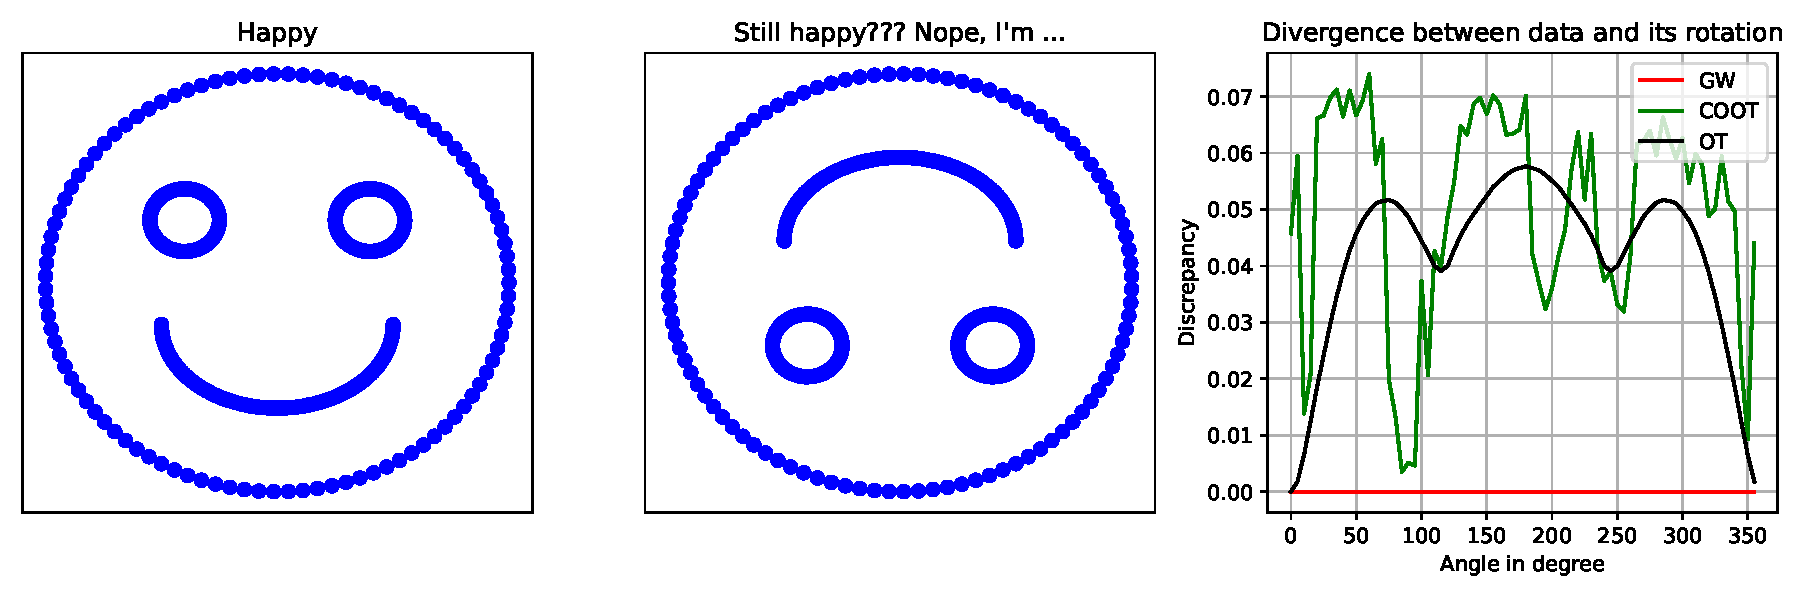
\includegraphics[width=1.\linewidth, keepaspectratio=true]{OT_new/div_vs_angle.pdf}
\end{figure}

\end{frame}

%%%%%%%%%%%%%%%%%%%%%%%%%%%%%%%%%%%%%%%%%%
\begin{frame}{Summary of contributions}
  \scriptsize

  \begin{tikzpicture}[remember picture, overlay]
    \node[shift={(0cm,-1.5cm)}] at (current page.center)
    {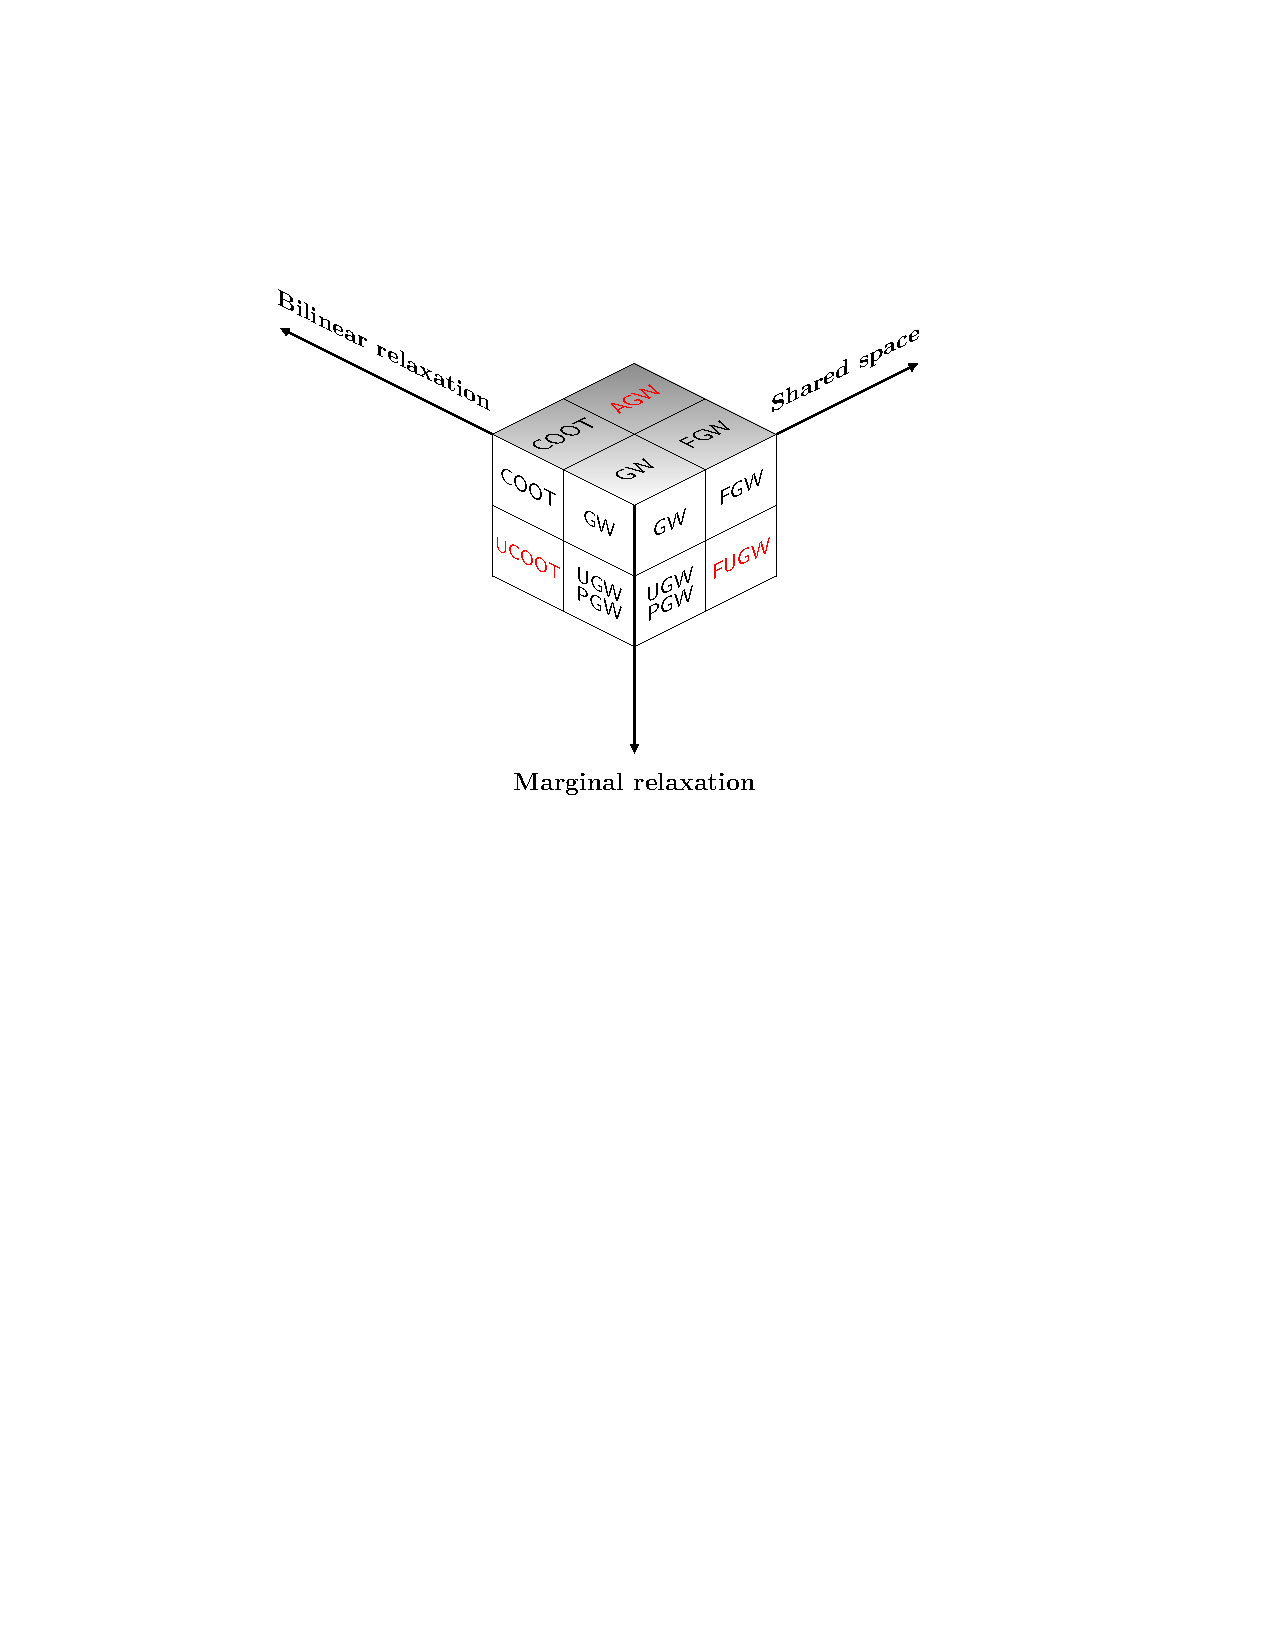
\includegraphics[scale=0.55]{OT_new/cube_agw_contrib.pdf}};
  \end{tikzpicture}

  \vspace{5cm}
  {\color{brown}{\textbf{Summary}}}:
  \begin{enumerate}
    \item Interpolation between GW and COOT to get the best from both worlds.
    \item Applications to heterogeneous domain adaptation and single-cell multi-omics.
  \end{enumerate}

  \vspace{0.3cm}
  {\color{brown}{\textbf{Publication}}}: \ul{Breaking isometric ties and introducing priors in Gromov-Wasserstein distances}.
  Pinar Demetci, \textbf{QHT}, Ievgen Redko, and Ritambhara Singh.
  \textit{International Conference on Artificial Intelligence and Statistics (AISTATS)}, 2024.

\end{frame}

%%%%%%%%%%%%%%%%%%%%%%%%%%%%%%%%%%%%%%
\begin{frame}{Formulation}
\scriptsize
\begin{block}{Definition}
  For $0\leq \alpha \leq 1$, the Augmented GW divergence between
  two weighted matrices $\cX_1 = (X_1, \mssrc, \mfsrc)$ and
  $\cX_2 = (X_2, \mstg, \mftg)$ is defined as
  \begin{align*}
    \label{eq:scootr}
    \agw_{\alpha}(\cX_1, \cX_2) &:=
    \min_{\substack{\pis \in U(\mssrc,\mstg) \\ \pif \in U(\mfsrc,\mftg)}}
    \alpha \cL_{\gw}(\pis) + (1-\alpha) \cL_{\coot}(\pis, \pif).
  \end{align*}
\end{block}

\begin{tikzpicture}[remember picture, overlay]
  \node[shift={(-3.7cm,-6cm)}] at (current page.center)
  {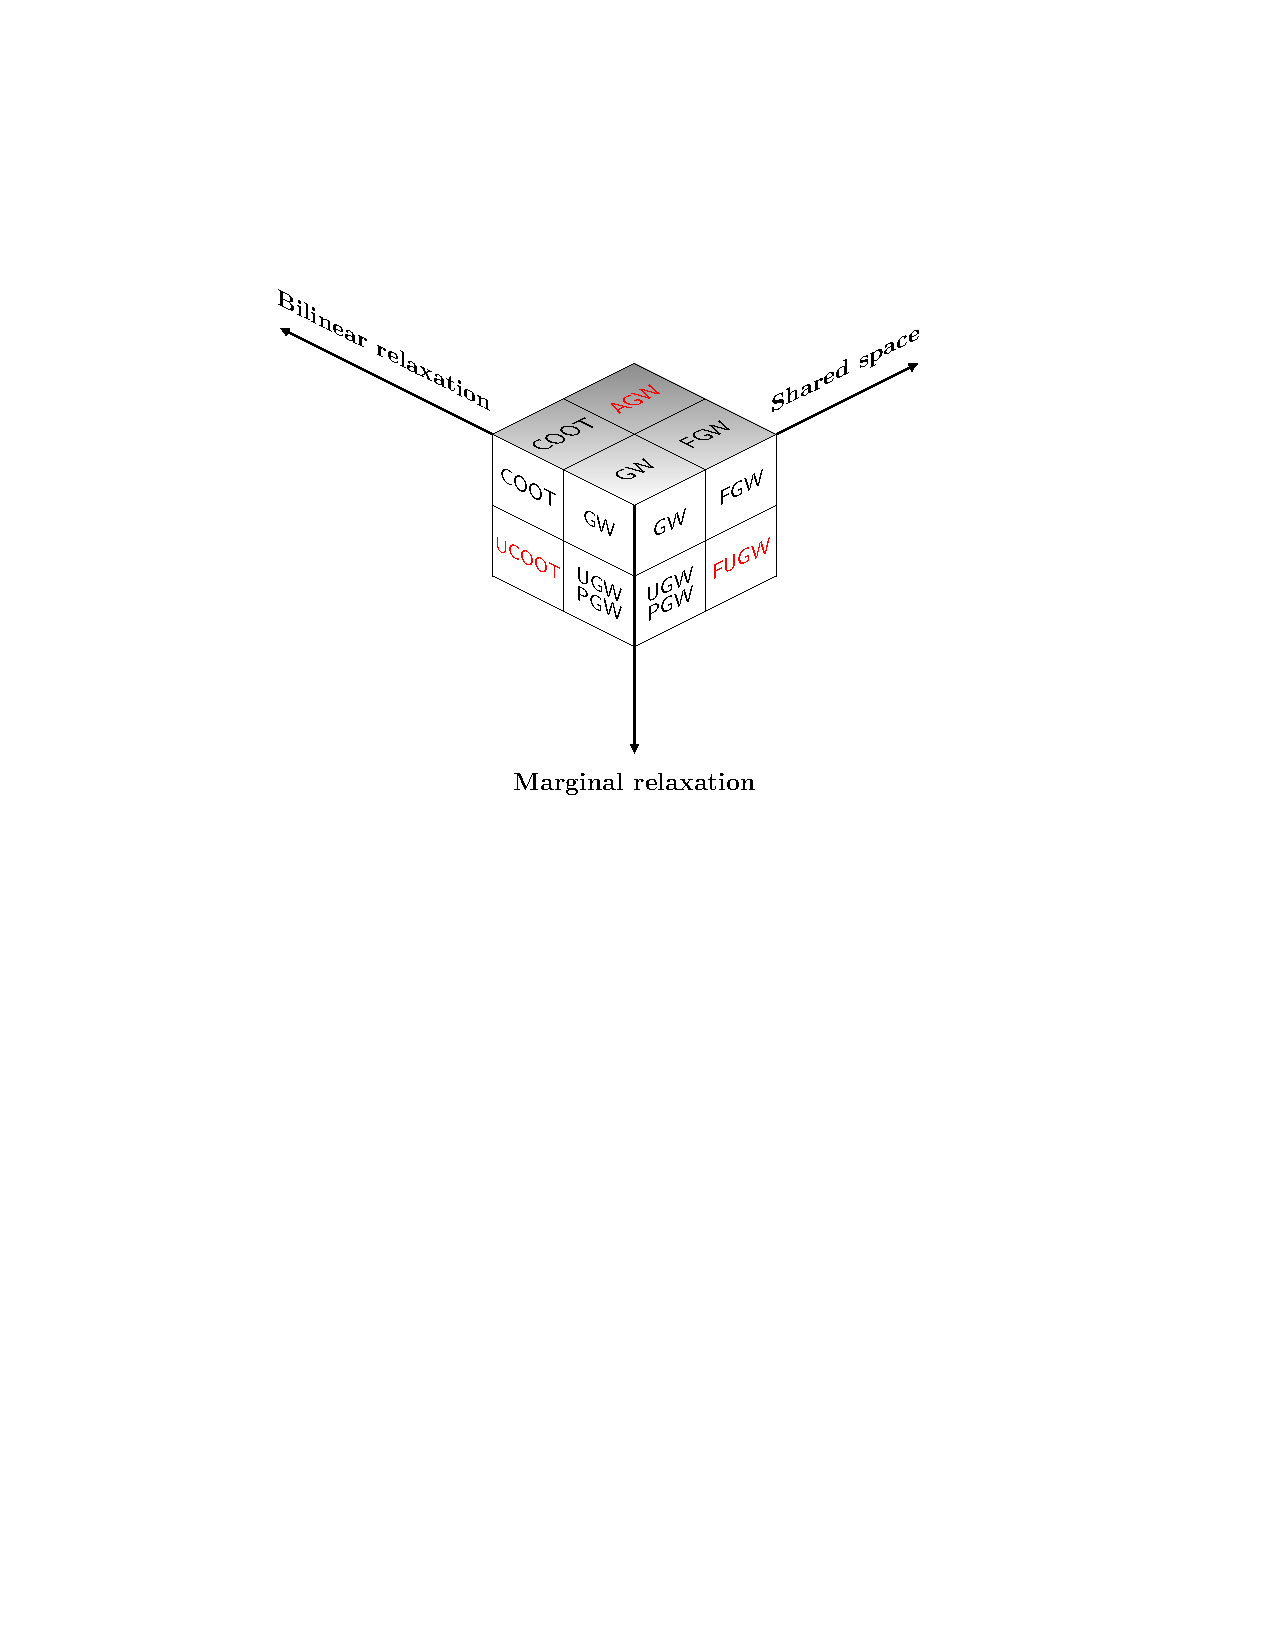
\includegraphics[scale=0.35]{OT_new/cube_agw.pdf}};
\end{tikzpicture}

\begin{minipage}[t]{0.55\linewidth}
  \begin{itemize}
    \item Interpolating between GW and COOT.
    \item Satisfying relaxed triangle inequality.
    \item Weak invariant to translation: shift minimum but leaves minimizer unchanged.
  \end{itemize}
  \end{minipage}%
  \hfill%
  \hspace{-6cm}
  \begin{minipage}[t]{0.45\linewidth}
    \vspace{-0.2cm}
  \begin{figure}
    \centering
    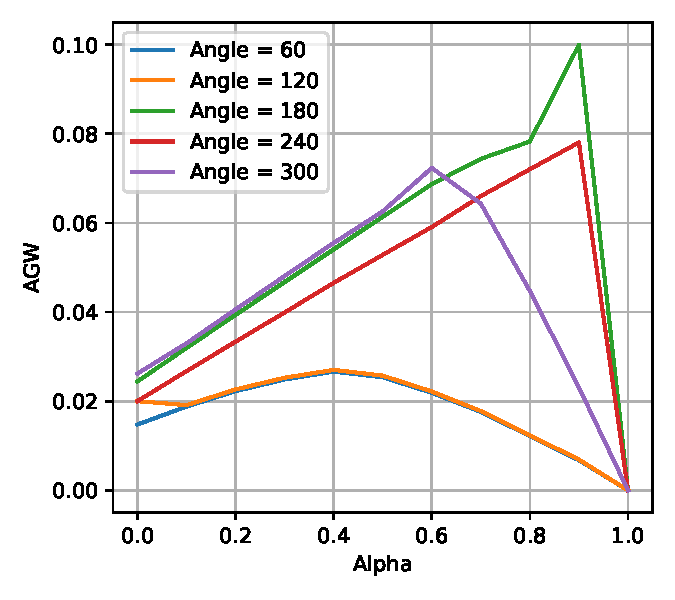
\includegraphics[width=1.15\linewidth, keepaspectratio=true]{OT_new/agw_alpha.pdf}
  \end{figure}
  \end{minipage}

\end{frame}

%%%%%%%%%%%%%%%%%%%%%%%%%%%%%%%%%%%%%%
\begin{frame}{Isometries}
\scriptsize
\vspace{-1cm}

\begin{assumption}
  \label{assumption:1}
Given an input matrix $X \in \bbR^{n \times d}$, assume
\begin{enumerate}
  \item[(A1)] $n \geq d$: Low-dimensional setting.
  \item[(A2)] $X$ is full rank: Easily met by preprocessing.
  \item[(A3)] $X$ has $d$ distinct singular values. Fact:
  set of Hermitian matrices with repeated eigenvalues has zero Lebesgue measure.
\end{enumerate}
\end{assumption}
\begin{proposition}
  Given two weighted matrices $\cX_1 = (X_1, \mssrc, \mfsrc)$
  and $\cX_2 = (X_2, \mstg, \mftg)$,
  \begin{enumerate}
      \item[$(\Rightarrow)$] If $\mssrc = \mstg$ and
      $X_2$ is obtained by permuting columns of $X_1$ via
      the permutation $\sigma_c$ (so $\mftg = (\sigma_c)_{\#} \mfsrc$),
      then $\agw_{\alpha}(\cX_1, \cX_2) = 0$.
      \item[$(\Leftarrow)$] Suppose $X_1$ satisfies A1-A3. For any $0 < \alpha < 1$,
      if $\agw_{\alpha}(\cX_1, \cX_2) = 0$,
      then there exist a symmetric orthogonal matrix $O \in \mathcal O_d$
      and a permutation matrix $P \in \mathcal P_d$ such that $X_2 = X_1 OP$.
  \end{enumerate}
\end{proposition}

\begin{tikzpicture}[remember picture, overlay]
  \node[shift={(-3.7cm,-6cm)}] at (current page.center)
  {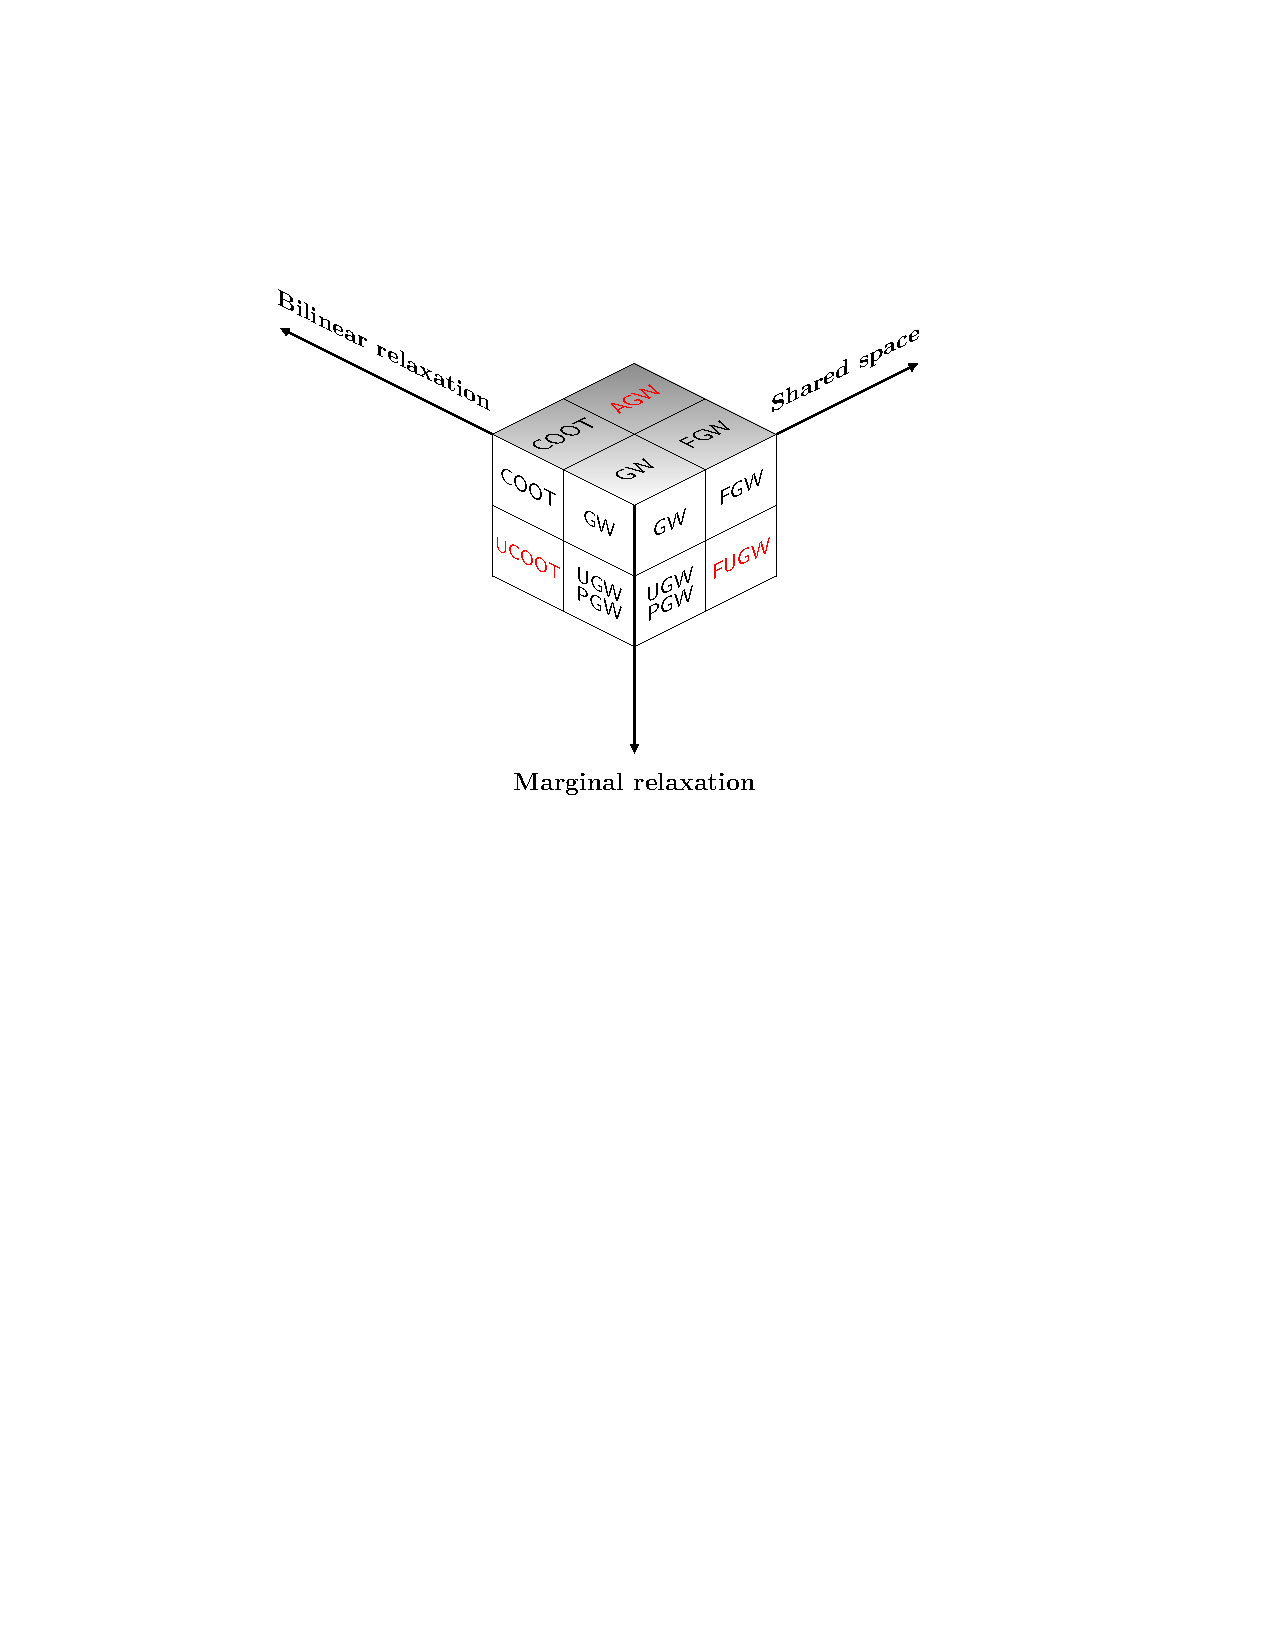
\includegraphics[scale=0.35]{OT_new/cube_agw.pdf}};
\end{tikzpicture}

\end{frame}

%%%%%%%%%%%%%%%%%%%%%%%%%%%%%%%%%
\begin{frame}{Single-cell multi-omics (with Pinar Demetci)}
\scriptsize
\vspace{-0.8cm}
\begin{itemize}
  \item Motivation: almost all current single-cell alignment methods only
  align samples (cells). Feature alignments can yield higher quality
  sample alignments.
  \item Dataset: CITE-Seq \parencite{CITEseq}
  \begin{itemize}
    \scriptsize
    \item Source: sample = cells, features = antibodies.
    \item Target: samples = same cells, features = gene expressions.
  \end{itemize}
\end{itemize}

\begin{figure}
  \centering
  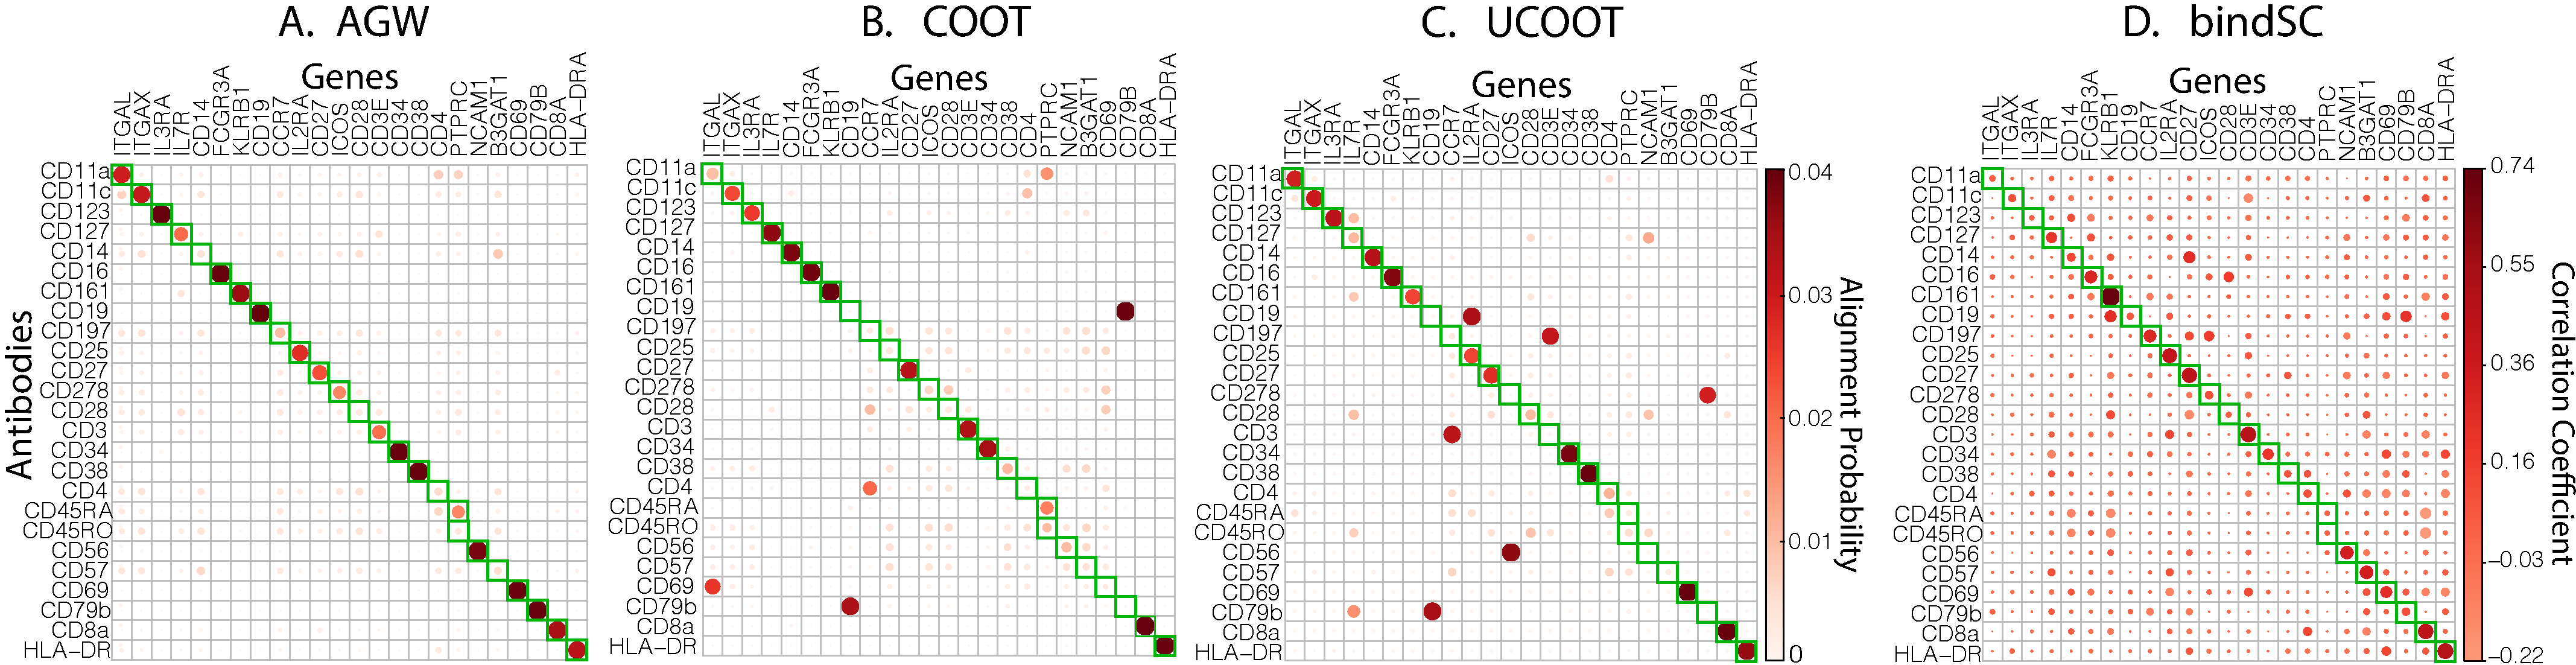
\includegraphics[width=1.\linewidth, keepaspectratio=true]{OT_new/cite_fgcoot_final.pdf}
  \caption*{\scriptsize{Feature alignments generated by competing methods.
  Green boxes indicate where we expect matches (“ground-truth”)
  based on domain knowledge.}}
\end{figure}

\begin{tikzpicture}[remember picture, overlay]
  \node[shift={(-3.7cm,-6cm)}] at (current page.center)
  {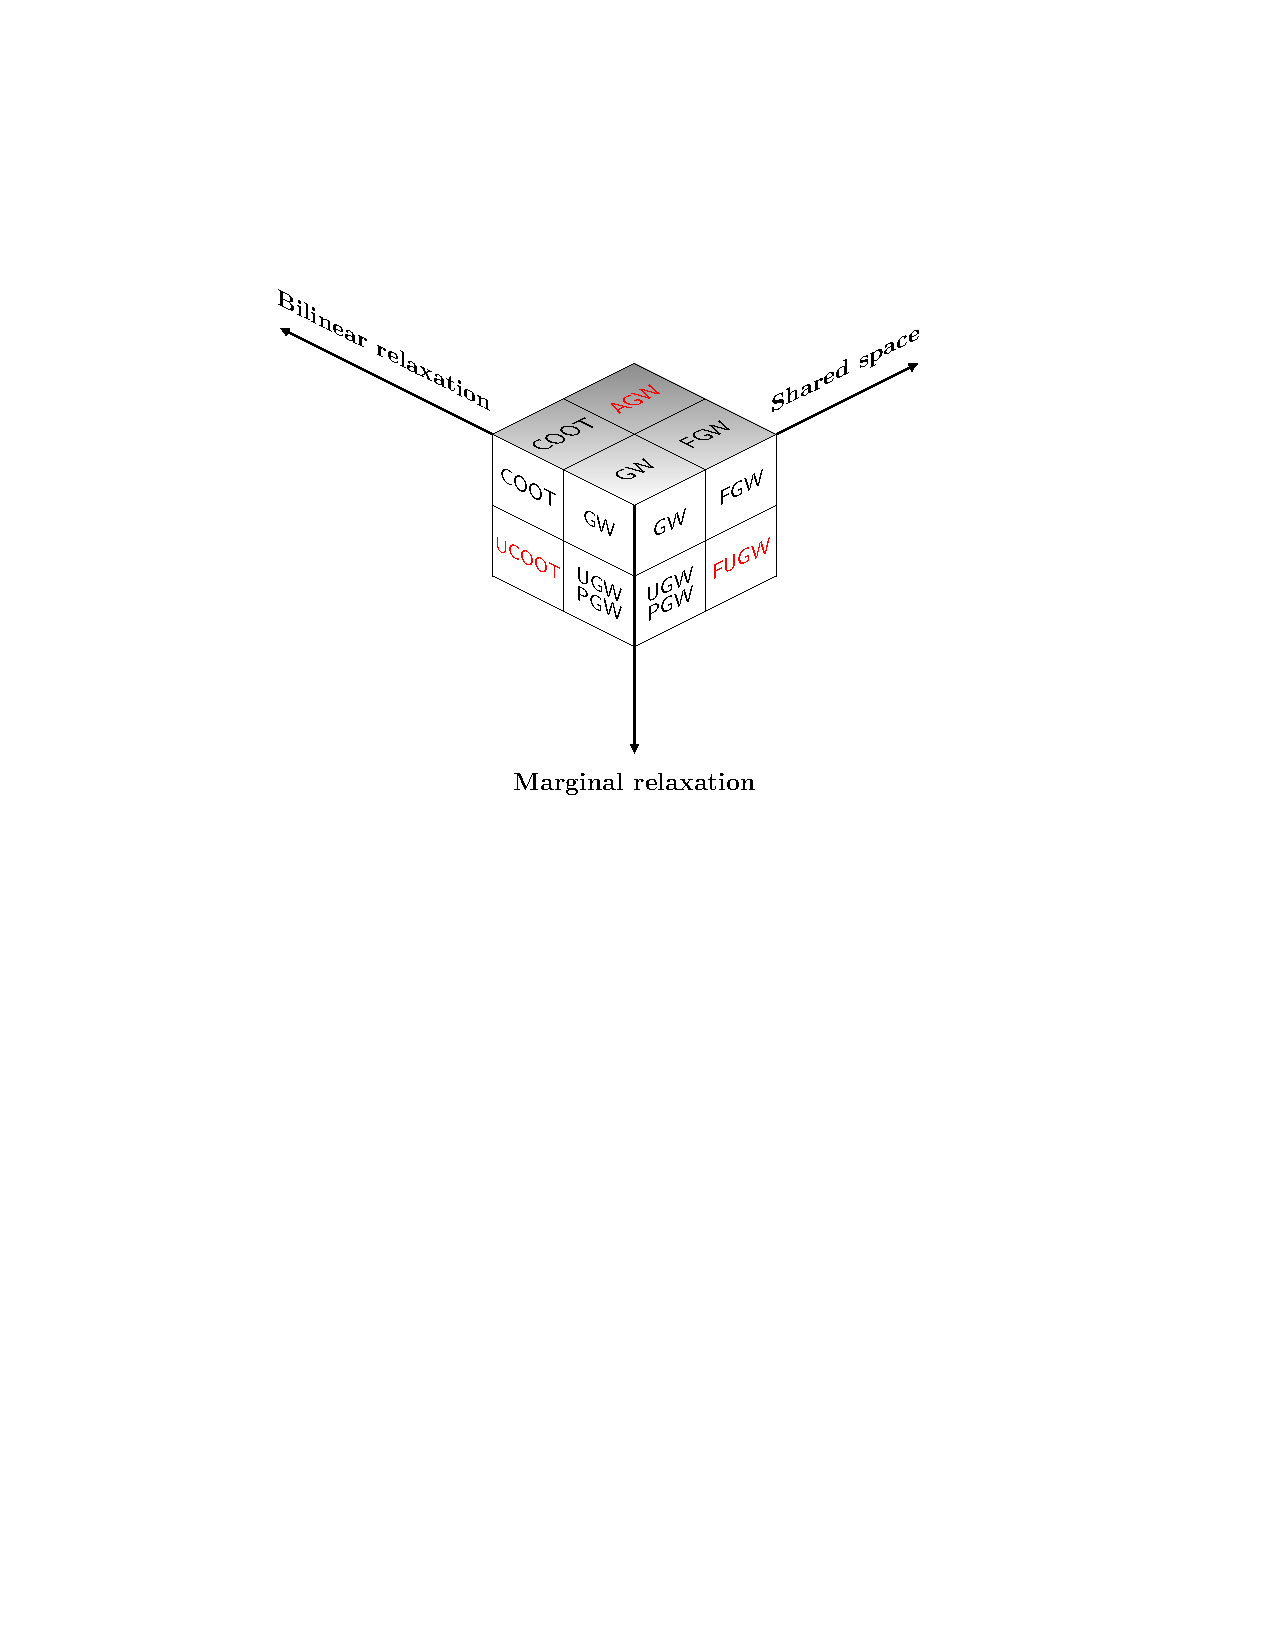
\includegraphics[scale=0.35]{OT_new/cube_agw.pdf}};
\end{tikzpicture}

\end{frame}

\section{Conclusion and Perspectives}
%%%%%%%%%%%%%%%%%%%%%%%%%%%%%%%%%%
\begin{frame}{Conclusion and Perspectives}
\scriptsize

{\color{brown}{\textbf{Conclusion}}}
\begin{enumerate}
  % \setlength\itemsep{0.5em}
  \item Filled the cube.
  \begin{itemize}
    \scriptsize
    \item FUGW (w/ Alexis Thual): \url{https://github.com/alexisthual/fugw}.
    \item UCOOT: \url{}.
    \item AGW: \url{}.
  \end{itemize}
  \item Established the robustness of unbalanced divergences.
  \item Real-world applications in neuroscience, domain adaptation and computational biology.
\end{enumerate}
\begin{tikzpicture}[remember picture, overlay]
  \node[shift={(6.5cm,-0.5cm)}] at (current page.center)
  {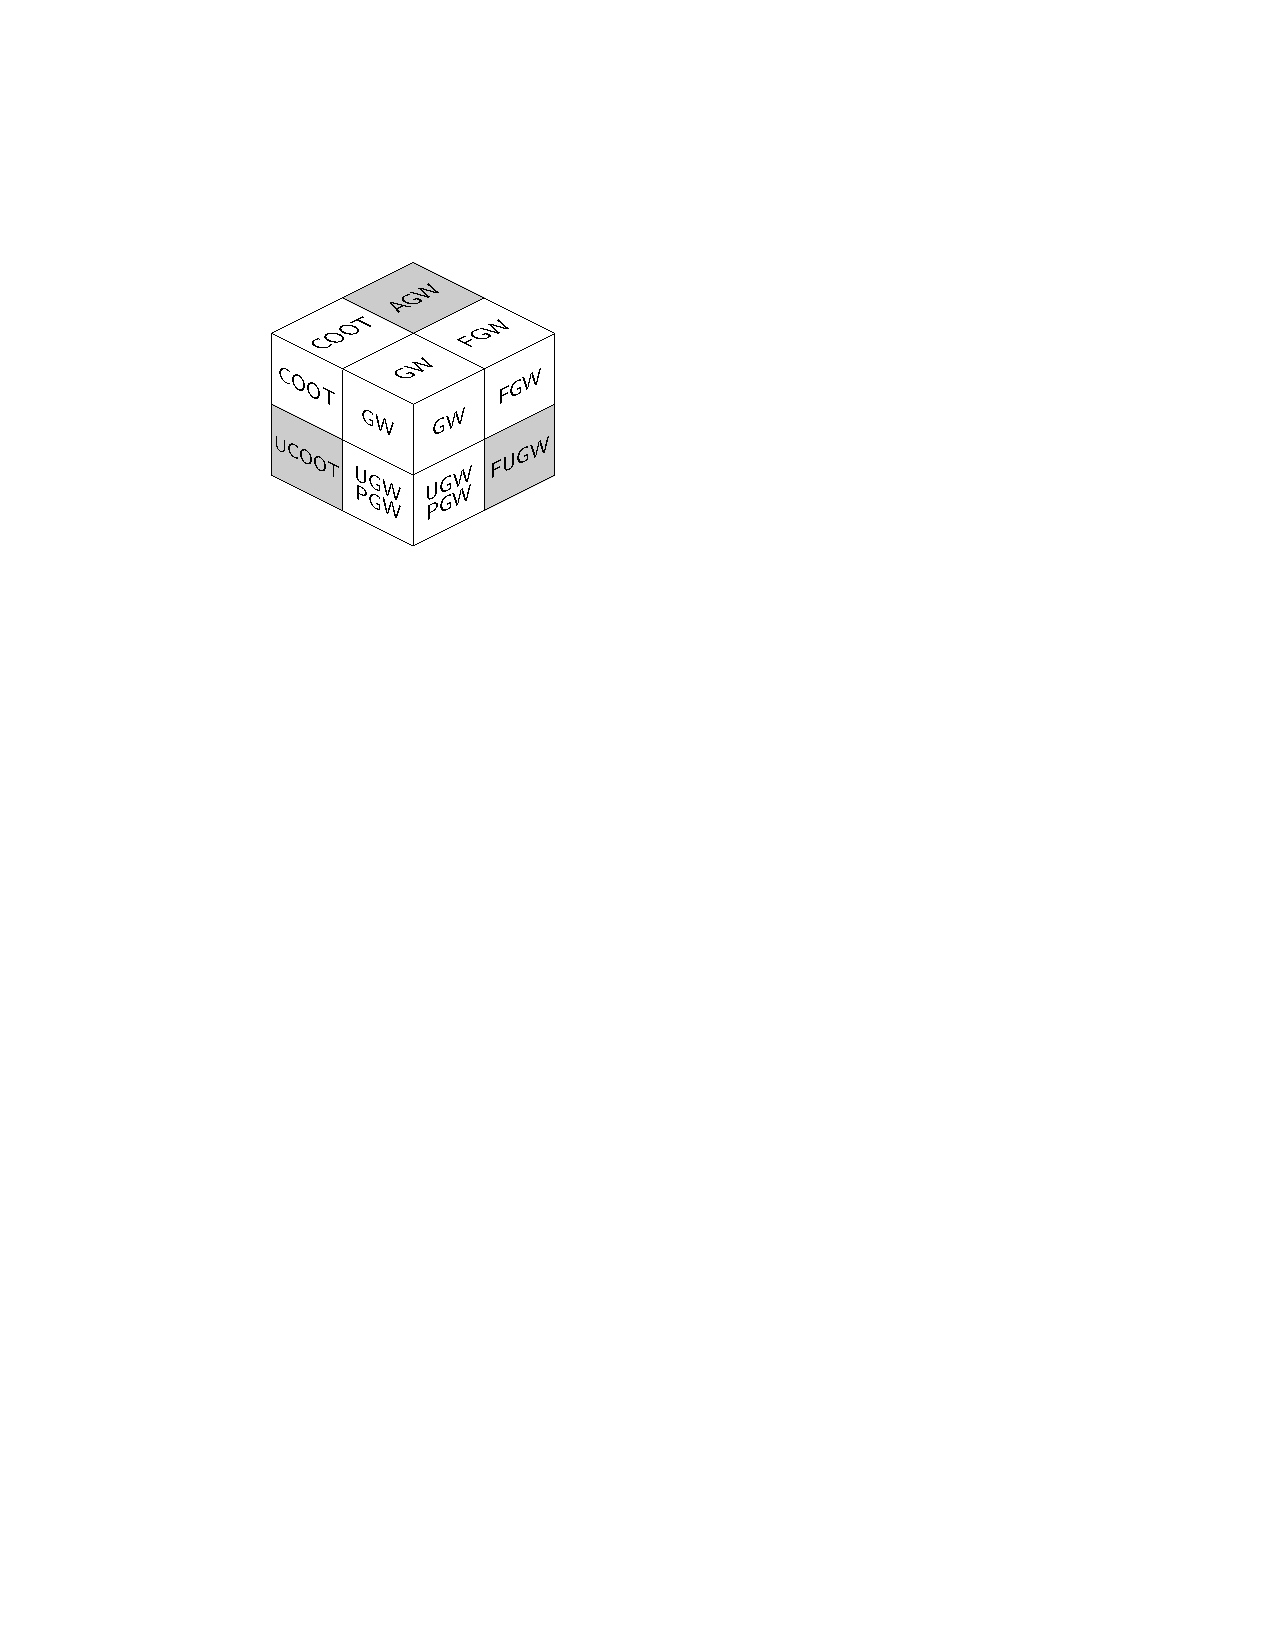
\includegraphics[scale=0.4]{OT_new/cube_summary.pdf}};
\end{tikzpicture}

\vspace{1cm}
{\color{brown}{\textbf{Perspectives}}}
\begin{enumerate}
  % \setlength\itemsep{0.5em}
  \item (Ongoing work) Fill the last missing corner.
  \item Isometries induced AGW is not fully understood.
  \item Statistical aspects of unbalanced across-space divergences
  are little explored.
  \item Algorithmic acceleration: UGW, FUGW, UCOOT rely on BCD

  $\Rightarrow$ More efficient UOT solvers.

  \begin{tikzpicture}[remember picture, overlay]
    \node[shift={(4cm,-4cm)}] at (current page.center)
    {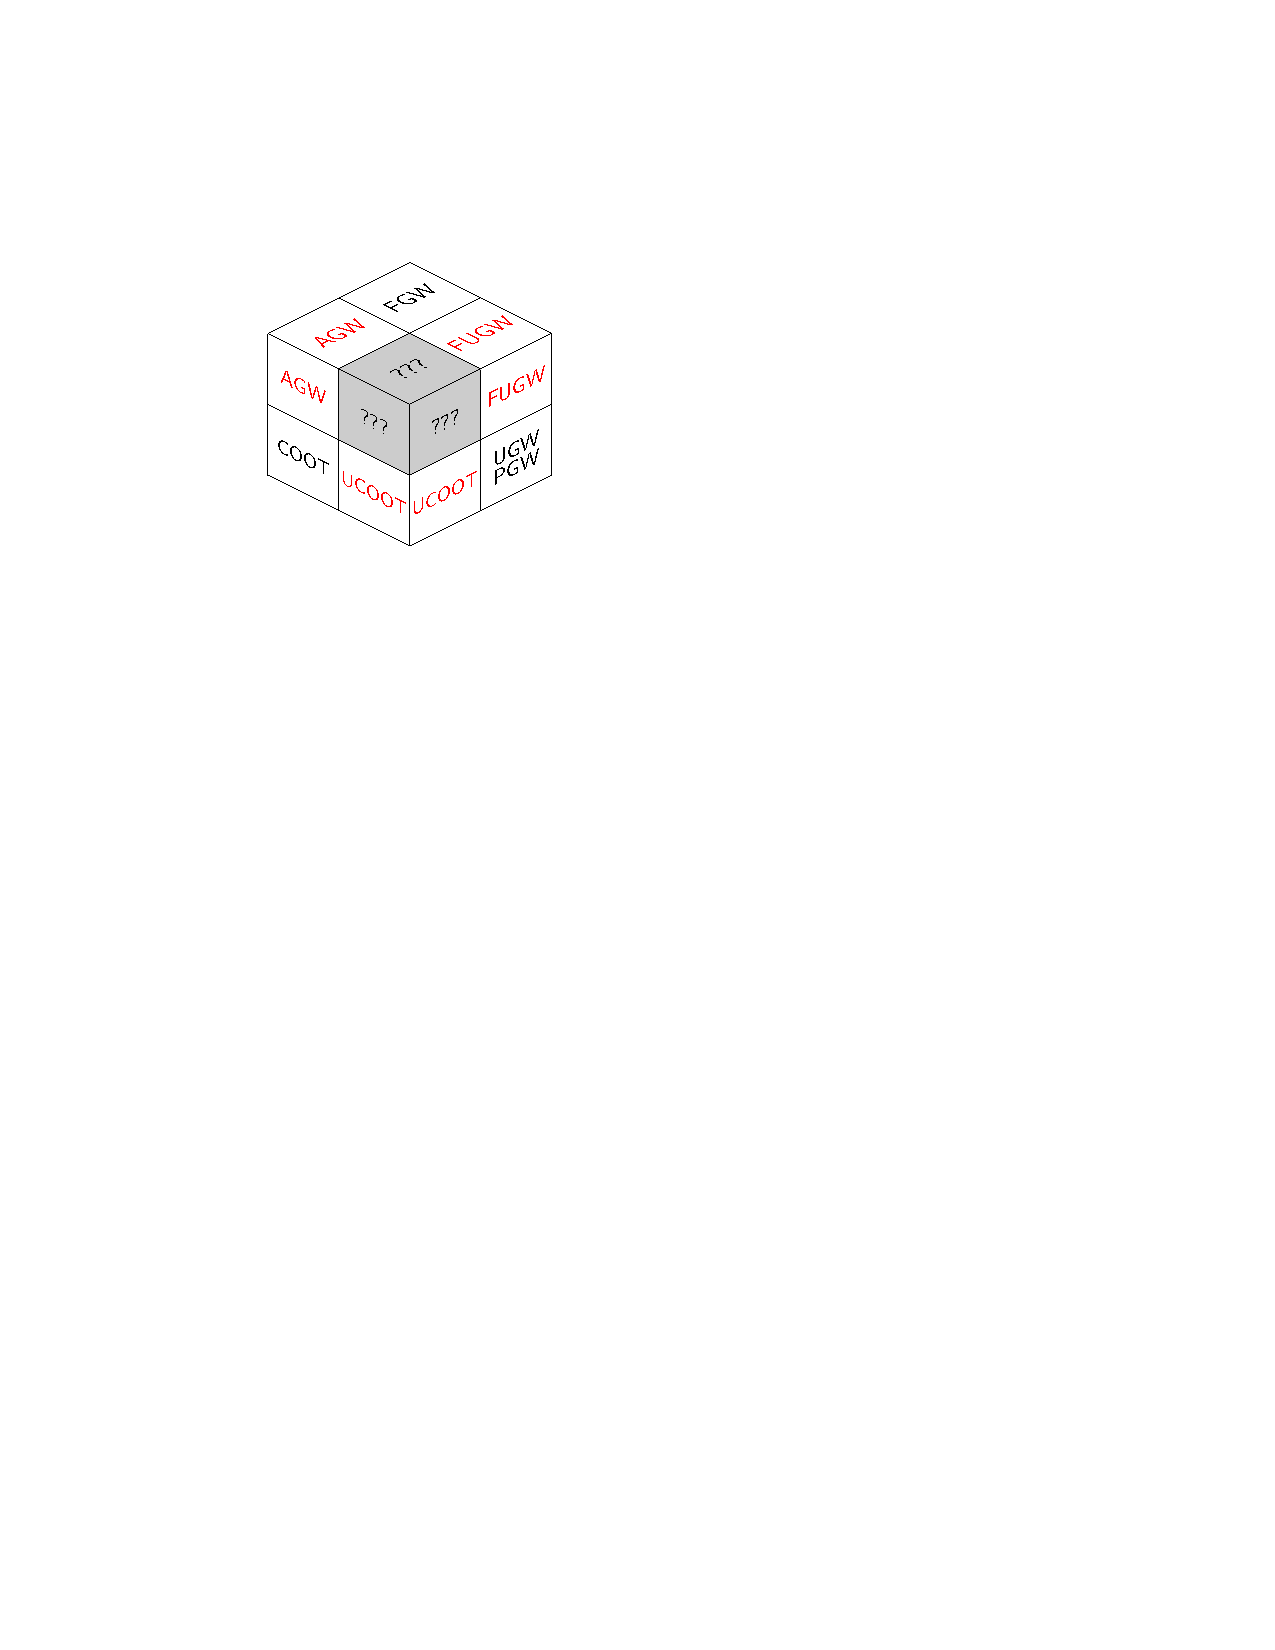
\includegraphics[scale=0.4]{OT_new/cube_future.pdf}};
  \end{tikzpicture}
\end{enumerate}

\end{frame}

%%%%%%%%%%%%%%%%%%%%%%%%%%%%%%%%%%
\begin{frame}
  \vspace{0.5cm}
  \centering \Large
  \textbf{{Thank you for your attention!}}

  \vspace{0.5cm}
  \begin{figure}
    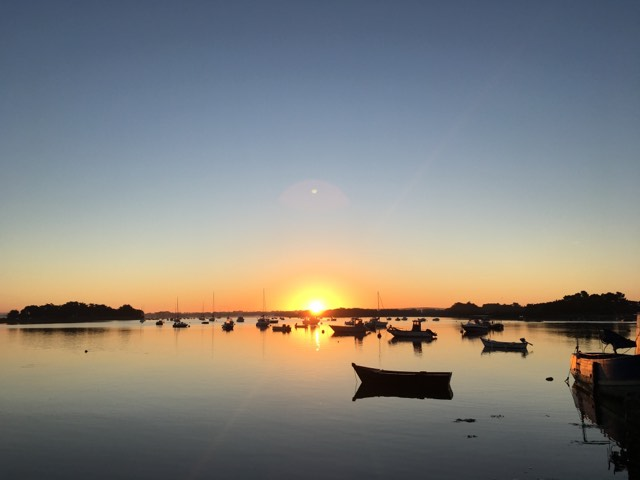
\includegraphics[scale=0.35]{OT_new/sunrise_vannes.jpg}
    \caption{Sunrise in Vannes, 24 September 2021}
    \label{fig1}
  \end{figure}
\end{frame}

%%%%%%%%%%%%%%%%%%%%%%%%%%%%%%
\section*{References}
%%%%%%%%%%%%%%%%%%%%%%%%%%%%%%%%%%%%%%%
\begin{frame}[allowframebreaks]{References}
\printbibliography
\end{frame}

%%%%%%%%%%%%%%%%%%%%%%%%%%%%%%%%%%%%%
\begin{frame}{Where Gromov-Wasserstein comes from?}
\scriptsize
%%%%%%%%%%%%%%%%%%%%%%%%%%%%%%%
\begin{minipage}[t]{0.6\linewidth}
  \begin{itemize}
    \item Hausdorff distance: $X, Y \subset (Z, d)$
    \vspace{-0.3cm}
    \begin{align*}
      d_{H}^{Z}\big( {\color{blue}{(X, d)}}, {\color{red}{(Y, d)}} \big)
      = \max \Big\{ \sup_{{\color{blue}{x \in X}}} d({\color{blue}{x}}, {\color{red}{Y}}),
      \sup_{{\color{red}{y \in Y}}} d({\color{red}{y}}, {\color{blue}{X}}) \Big\}.
    \end{align*}
    \begin{tikzpicture}[remember picture, overlay]
      \node[shift={(4cm,-0.3cm)}] at (current page.center)
      {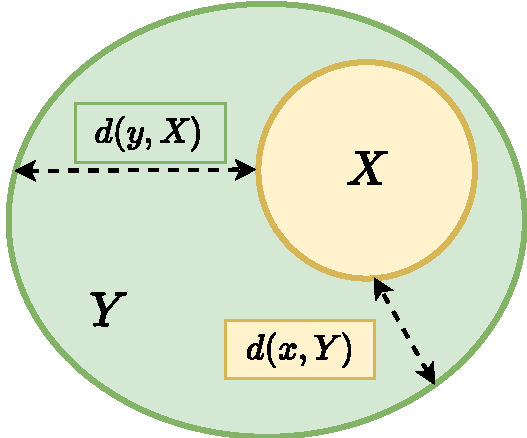
\includegraphics[scale=0.3]{OT_new/haus.pdf}};
    \end{tikzpicture}

    \vspace{-0.4cm}
    \item Gromov-Hausdorff distance \parencite{Gromov81,Gromov99}
    \vspace{-0.3cm}
    \begin{align*}
      \gh \big( {\color{blue}{(X, d_X)}}, {\color{red}{(Y, d_Y)}} \big) =
      \inf_{\substack{\text{met.sp.}(Z, d) \\
      \text{iso.} {\color{blue}{f: X}} \to Z \\
      \text{iso.} {\color{red}{g: Y}} \to Z}}
      d_{H}^{Z} \Big( {\color{blue}{\big(f(X), d \big)}}, {\color{red}{\big(g(Y), d \big)}} \Big).
      \end{align*}
      \begin{tikzpicture}[remember picture, overlay]
      \node[shift={(4.3cm,-2.9cm)}] at (current page.center)
      {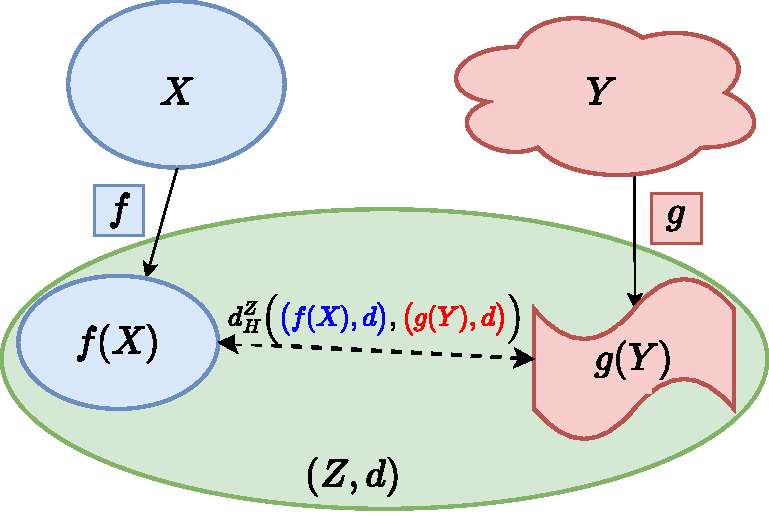
\includegraphics[scale=0.3]{OT_new/ghaus.pdf}};
    \end{tikzpicture}
  \end{itemize}
  \end{minipage}%

  \hfill%
  \hspace{-6cm}
  \begin{minipage}[t]{0.5\linewidth}
\end{minipage}
\vspace{1cm}

\end{frame}

%%%%%%%%%%%%%%%%%%%%%%%%%%%%%%%%%%%%
\begin{frame}
  \scriptsize
  \begin{tikzpicture}[remember picture, overlay]
    \node[shift={(0cm,0.3cm)}] at (current page.center)
    {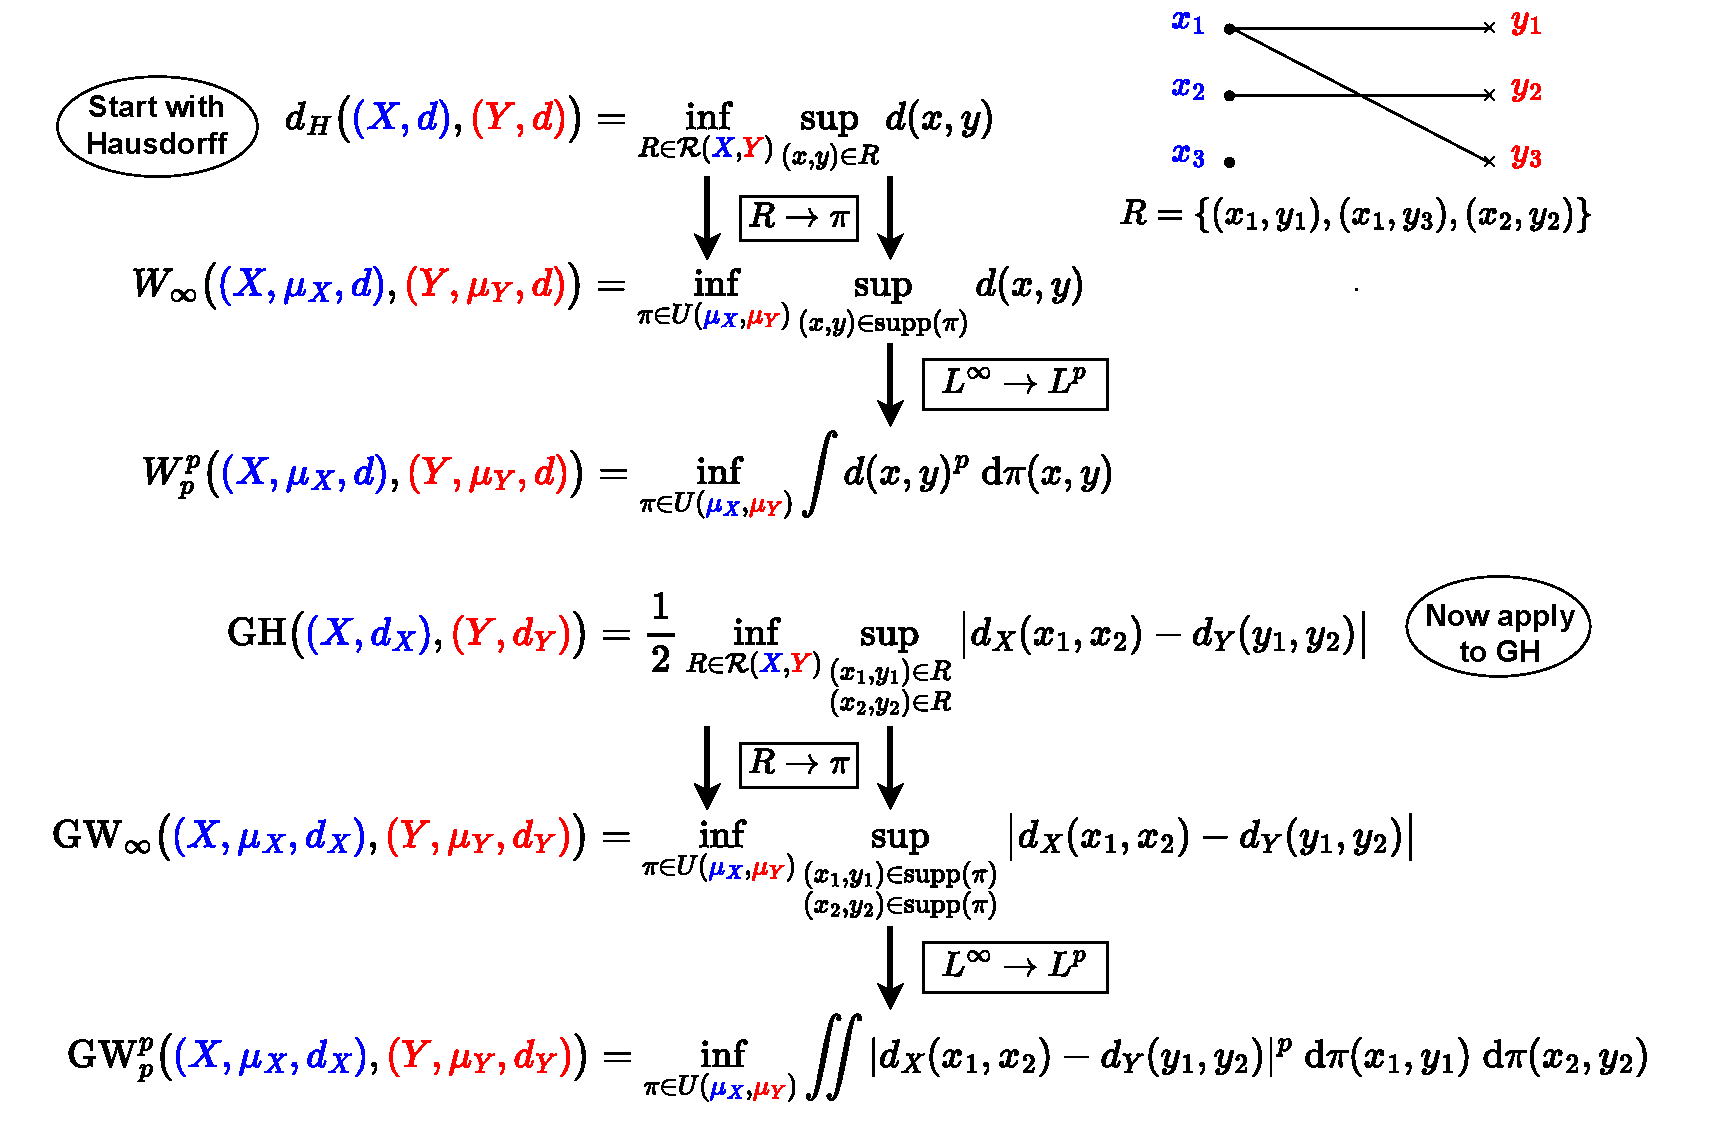
\includegraphics[scale=0.45]{OT_new/gww.pdf}};
    \begin{pgfinterruptboundingbox}
        \fill <1> [fill=white, opacity=0.85] (-1,-0.5) rectangle (12, -5);
    \end{pgfinterruptboundingbox}
    % \node <1> [draw, shape=rectangle, align=right] at (10, 5) {%
    %     Hello from outliers
    % };
  \end{tikzpicture}
\end{frame}

%%%%%%%%%%%%%%%%%%%%%%%%%%%%%%%%%%%%%
\begin{frame}
  \begin{tikzpicture}[remember picture, overlay]
    \node[shift={(0cm,0.3cm)}] at (current page.center)
    {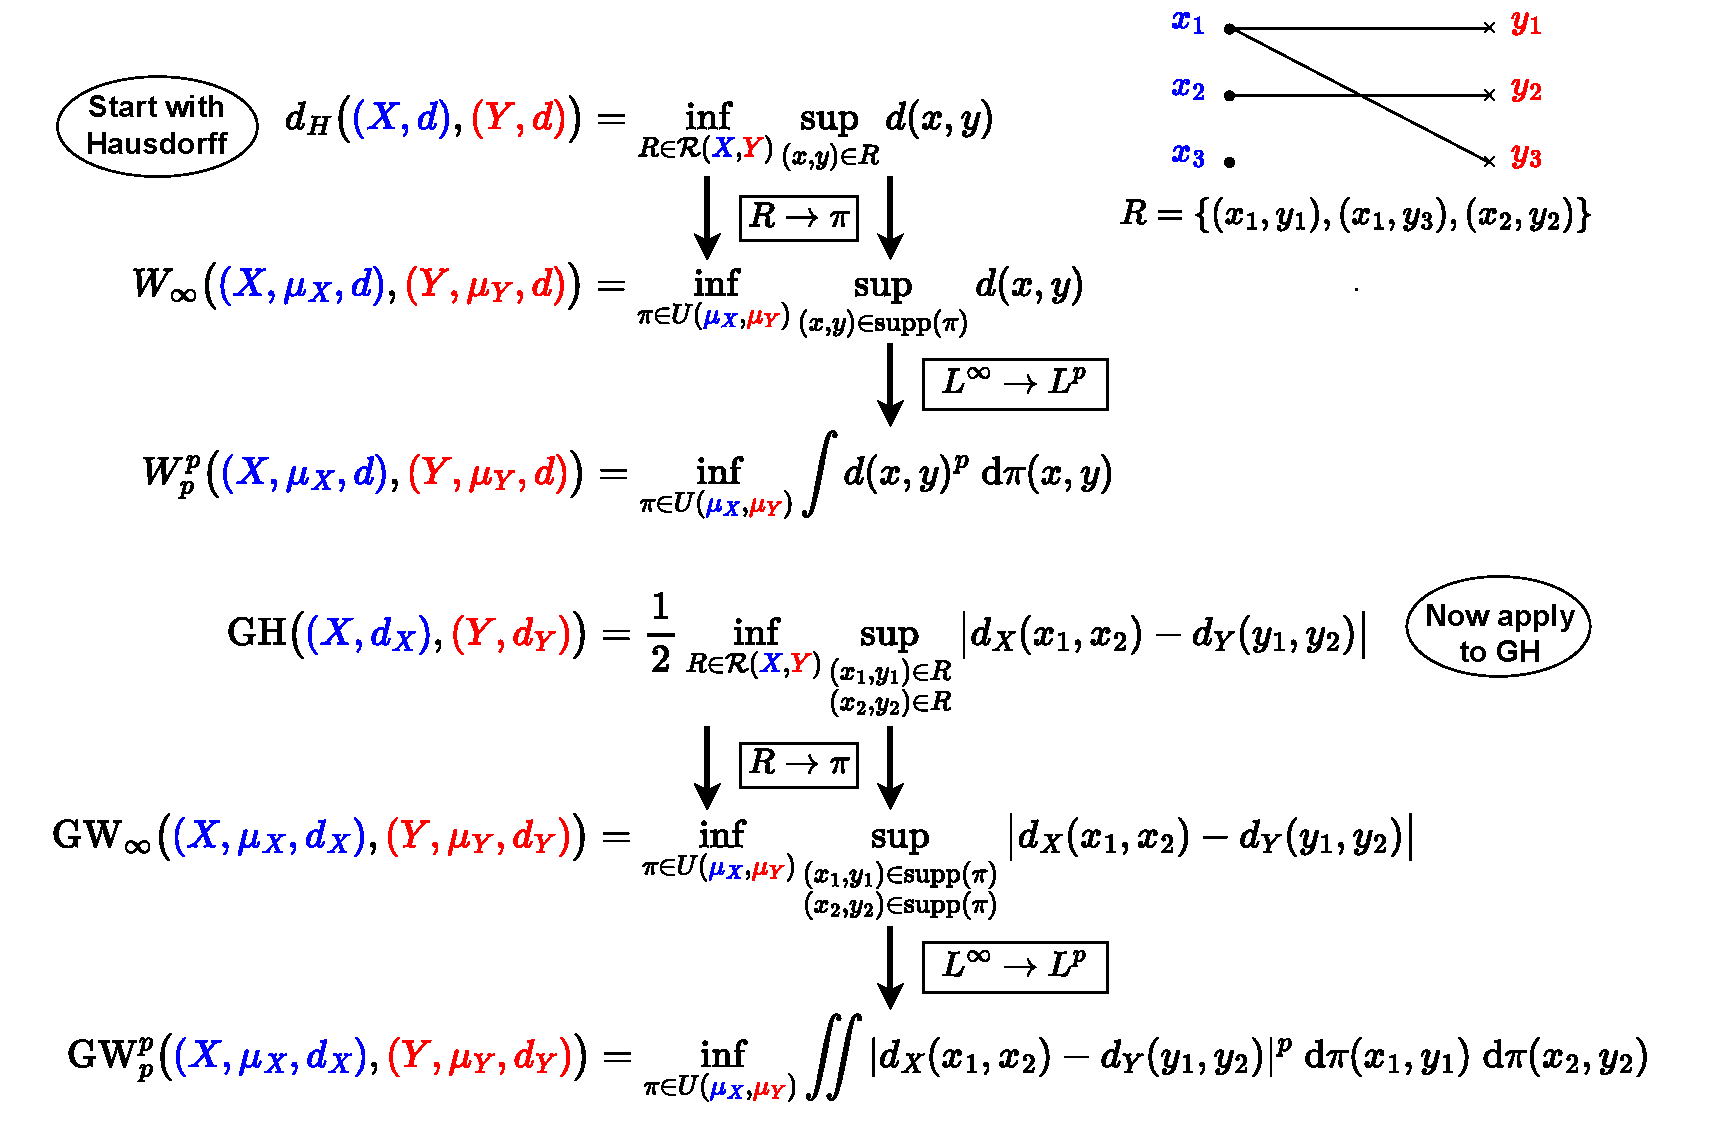
\includegraphics[scale=0.45]{OT_new/gww.pdf}};
  \end{tikzpicture}
\end{frame}

%%%%%%%%%%%%%%%%%%%%%%%%%%%%%%%%%%%%%%%
\begin{frame}{Why quadratic divergence?}
  \scriptsize
  \vspace{-1cm}
\begin{enumerate}
  \item Homogeneity:
  for $t\cX = \left({\color{blue}{(X^s, t\mu^s)}}, {\color{red}{(X^f, t\mu^f)}}, \xi \right)$
  \begin{align*}
    \ucoot_{\lambda}(t\cX_1, t\cX_2) = t^2 \ucoot_{\lambda}(\cX_1, \cX_2).
  \end{align*}
  $\Rightarrow$ Due to the property of Csiszár divergence.

  \item UCOOT = UOT under additional factorization constraint
  $\Rightarrow$ Existence of solution.

  \item Bilinear relation between minimum and minimizer.
  \begin{align*}
    \ucoot_{\lambda}(\cX_1, \cX_2) =
    \sum_{k=1}^2 \lambda_k m({\color{blue}{\mu_k^s}}) m({\color{red}{\mu_k^f}})
    - (\lambda_1 + \lambda_2) m({\color{blue}{\pi^s_*}}) m({\color{red}{\pi^f_*}}).
  \end{align*}
  $\Rightarrow$ Due to the property of Bregman divergence.

  \item Restriction to equal-mass solutions: $m({\color{blue}{\pi^s_*}}) = m({\color{red}{\pi^f_*}})$.

  $\Rightarrow$ Numerical stability when solving with entropic regularization.

  \item Provable robustness to outliers.
\end{enumerate}

\begin{tikzpicture}[remember picture, overlay]
  \node[shift={(-3.7cm,-6cm)}] at (current page.center)
  {\includegraphics[scale=0.35]{OT_new/cube_ucoot.pdf}};
\end{tikzpicture}

\end{frame}

\end{document}